\appendix

\chapter{Additional Listings}

\begin{lstlisting}[language=C, caption={Example usage of Repetition Test Library}, label={lst:reptest_example}]
// NOTE: Define the interface that all the functions we want to test conform to.
typedef void (*Test_Function)(u8 *buffer, usize buffer_size);
static
void read_buffer_linearly(u8 *buffer, usize buffer_size)
{
  ... // Omitted for brevity
}
static
void read_buffer_randomly(u8 *buffer, usize buffer_size)
{
  ... // Omitted for brevity
}

// NOTE: Each entry is just going to be the function and
// then a little string to name it.
typedef struct Function_Entry Function_Entry;
struct Function_Entry
{
  const char    *name;
  Test_Function function;
};
// NOTE: Ok now we can just make an array of all the functions we want to test.
Function_Entry entries[] =
{
  {"linearly", read_buffer_linearly},
  {"randomly", read_buffer_randomly},
};

int main(int argc, char **argv)
{
  Arena arena = arena_make(.reserve_size = GB(64));
  u64 cpu_timer_frequency = estimate_cpu_timer_freq();

  // NOTE: How many seconds to keep trying for a new min, will reset once
  // we find a new minimum.
  u32 seconds_to_try_for_min = 1;

  // NOTE: User may provide custom fields.
  Repetition_Series *series = repetition_series_make(60 * STATIC_COUNT(entries), ((const char *[]){"buffer_size", "function"}));

  for (usize buffer_size = MB(1); buffer_size <= MB(4); buffer_size *= 4)
  {
    for (usize test_func_idx = 0; test_func_idx < STATIC_COUNT(entries); test_func_idx++)
    {
      // NOTE: Allocating and deallocating every time to make it fair page-fault wise.
      u8 *buffer = os_allocate(buffer_size, OS_ALLOCATION_COMMIT);

      Function_Entry *entry = &entries[test_func_idx];

      Repetition_Tester tester = repetition_series_new_tester(series, buffer_size,
                                                              cpu_timer_frequency,
                                                              seconds_to_try_for_min,
                                                              "--- %s @ %lu MB ---", entry->name,
                                                              buffer_size / MB(1));

      // NOTE: User may set fields of current test.
      repetition_series_set_field(series, "buffer_size", "%lu", buffer_size);
      repetition_series_set_field(series, "function", entry->name);

      // NOTE: The main loop, it will continue testing until the minimum time has not decreased in user-provided time-frame.
      while (repetition_series_is_testing(series, &tester))
      {
        repetition_tester_begin_time(&tester);
        entry->function(buffer, buffer_size);
        repetition_tester_close_time(&tester);

        repetition_tester_count_bytes(&tester, buffer_size);
      }

      os_deallocate(buffer, buffer_size);
    }
  }

  // NOTE: Self-explanatory
  repetition_series_save_csv(series, "out.csv");
}
\end{lstlisting}

\chapter{Format Comparison Figures}
\label{app:format_figs}

\begin{figure}[htbp]
    \centering
    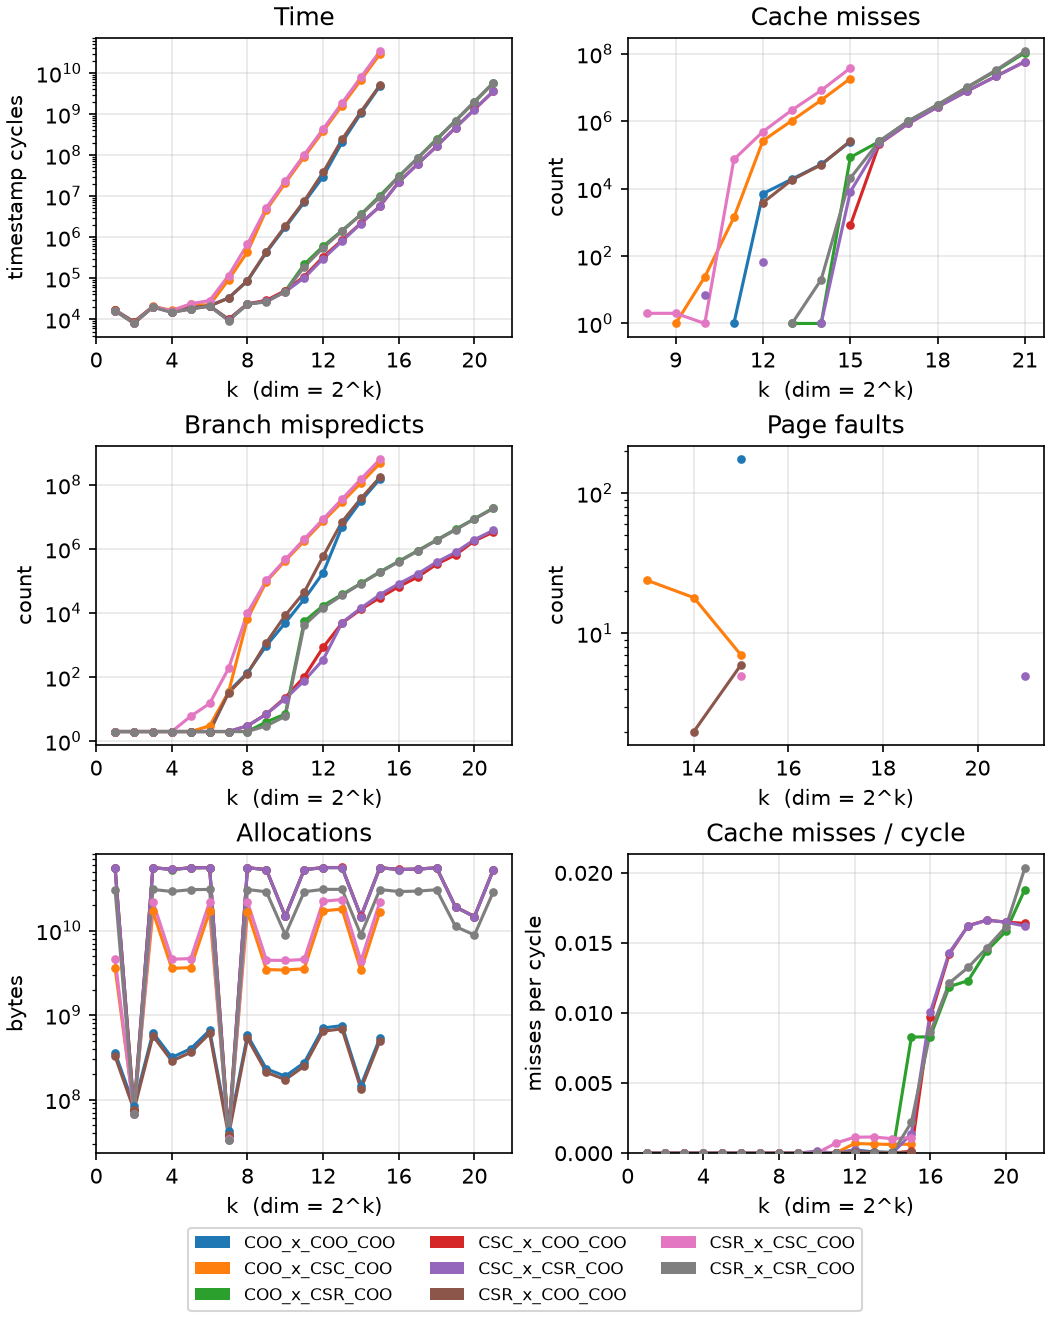
\includegraphics[width=0.85\linewidth,height=0.75\textheight,keepaspectratio]{figures/formats_AS-Newman_s2.png}
    \caption{AS-Newman Sample 2 comparison.}
    \label{fig:formats_AS-Newman}
\end{figure}

\begin{figure}[htbp]
    \centering
    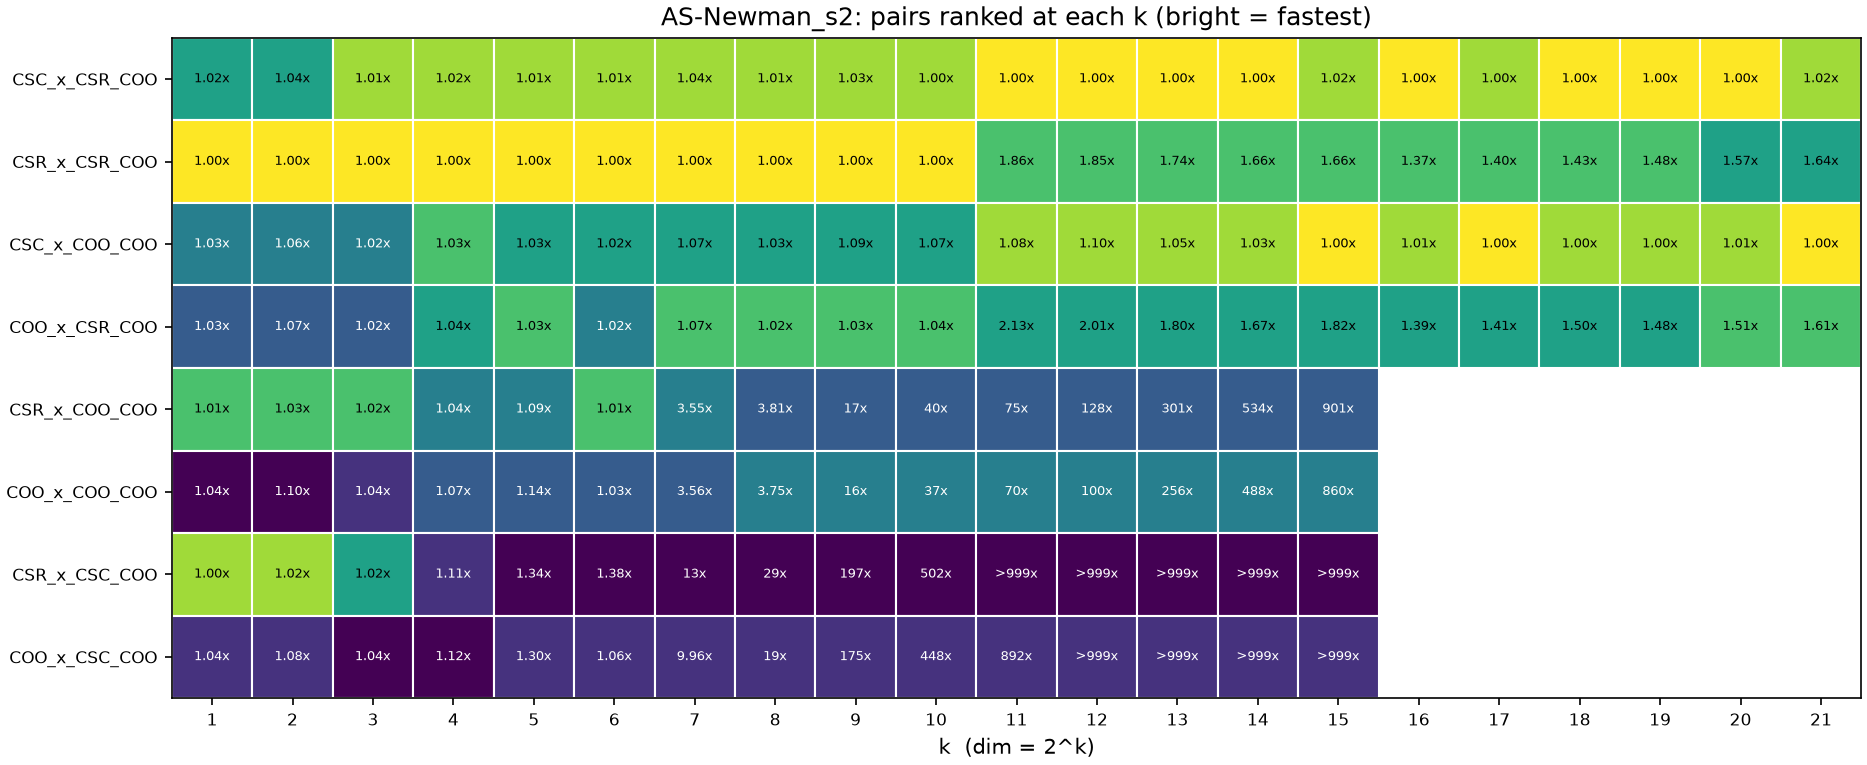
\includegraphics[width=\linewidth,height=0.6\textheight,keepaspectratio]{figures/formats_ranks_AS-Newman_s2.png}
    \caption{AS-Newman Sample 2: format pairs ranked at each $k$. Brighter cells are faster; each number is the slowdown relative to the fastest pair at that $k$.}
    \label{fig:formats_ranks_AS-Newman}
\end{figure}
\clearpage

\begin{figure}[htbp]
    \centering
    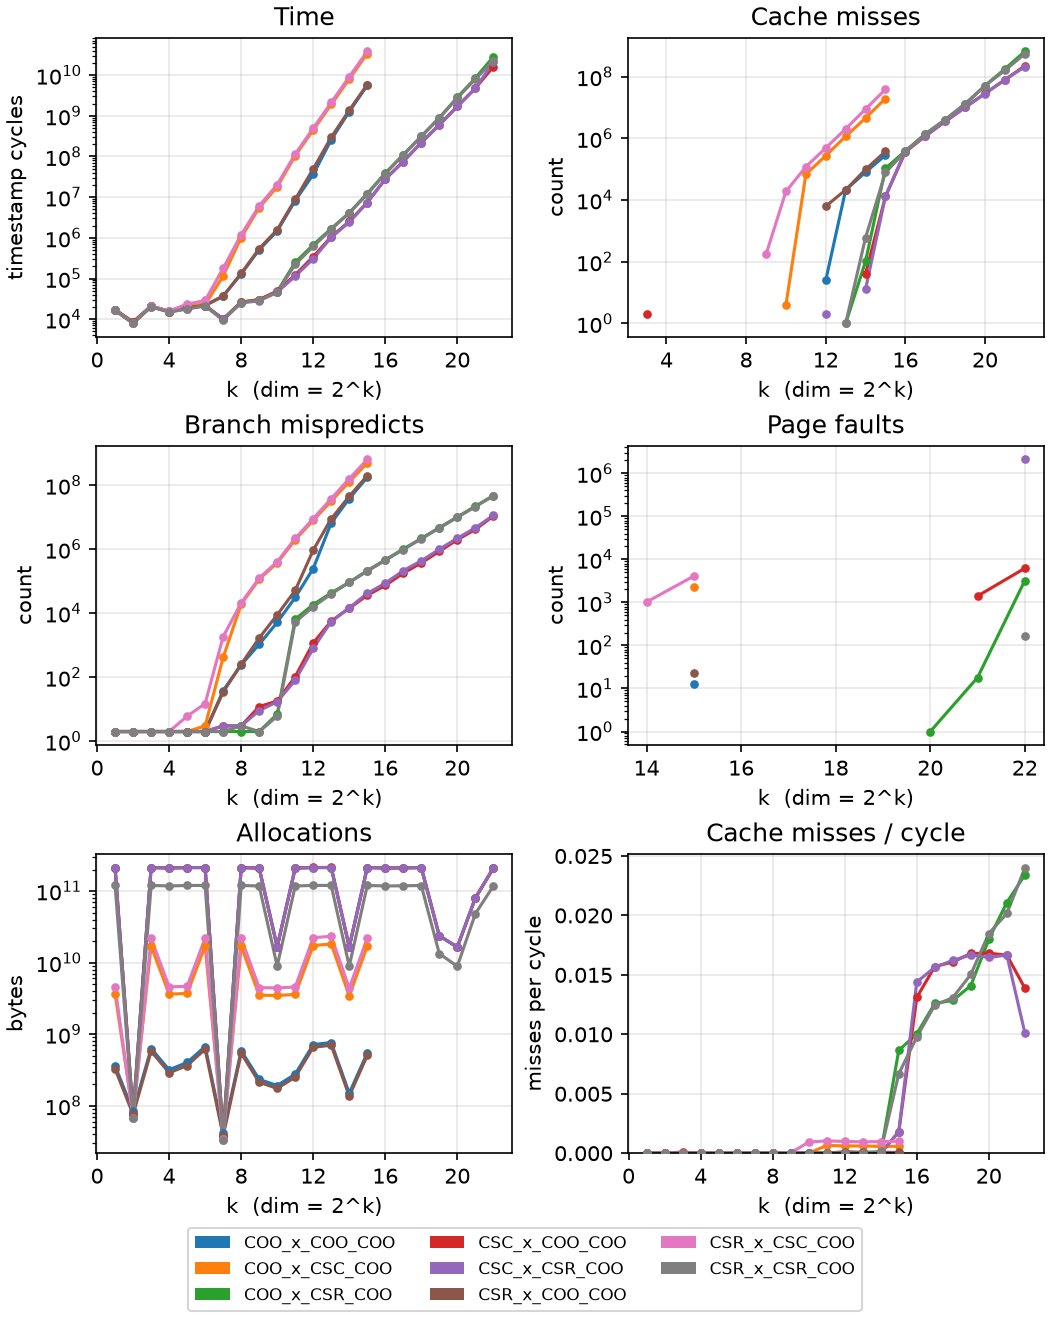
\includegraphics[width=0.85\linewidth,height=0.75\textheight,keepaspectratio]{figures/formats_AS-RouteViews_s2.png}
    \caption{AS-RouteViews Sample 2 comparison.}
    \label{fig:formats_AS-RouteViews}
\end{figure}

\begin{figure}[htbp]
    \centering
    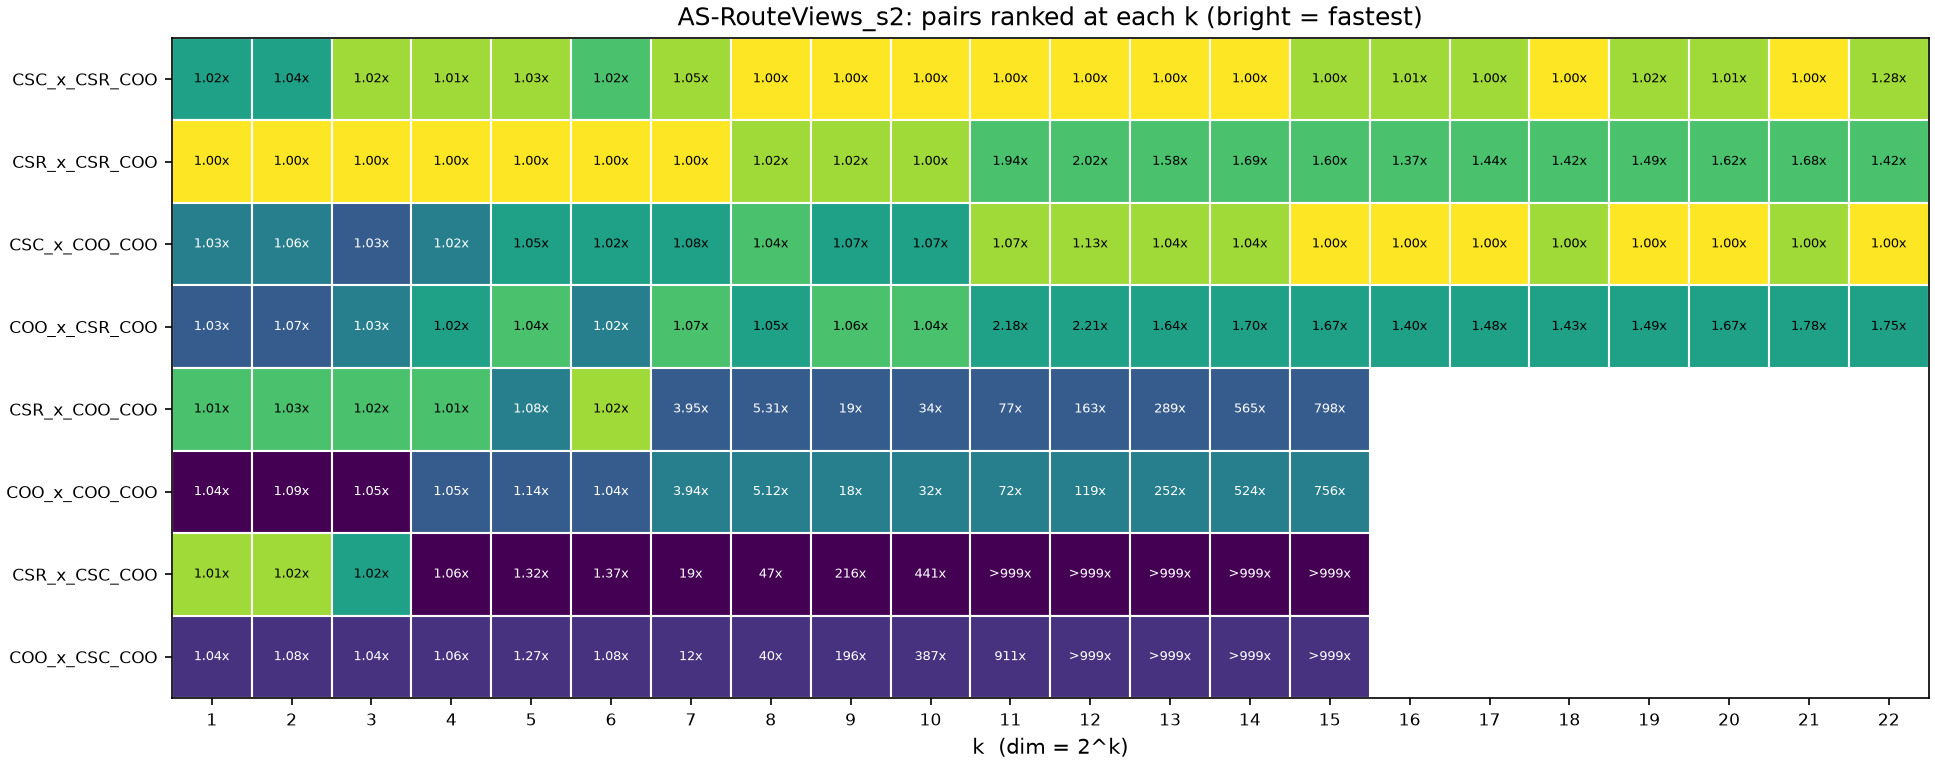
\includegraphics[width=\linewidth,height=0.6\textheight,keepaspectratio]{figures/formats_ranks_AS-RouteViews_s2.png}
    \caption{AS-RouteViews Sample 2: format pairs ranked at each $k$. Brighter cells are faster; each number is the slowdown relative to the fastest pair at that $k$.}
    \label{fig:formats_ranks_AS-RouteViews}
\end{figure}
\clearpage

\begin{figure}[htbp]
    \centering
    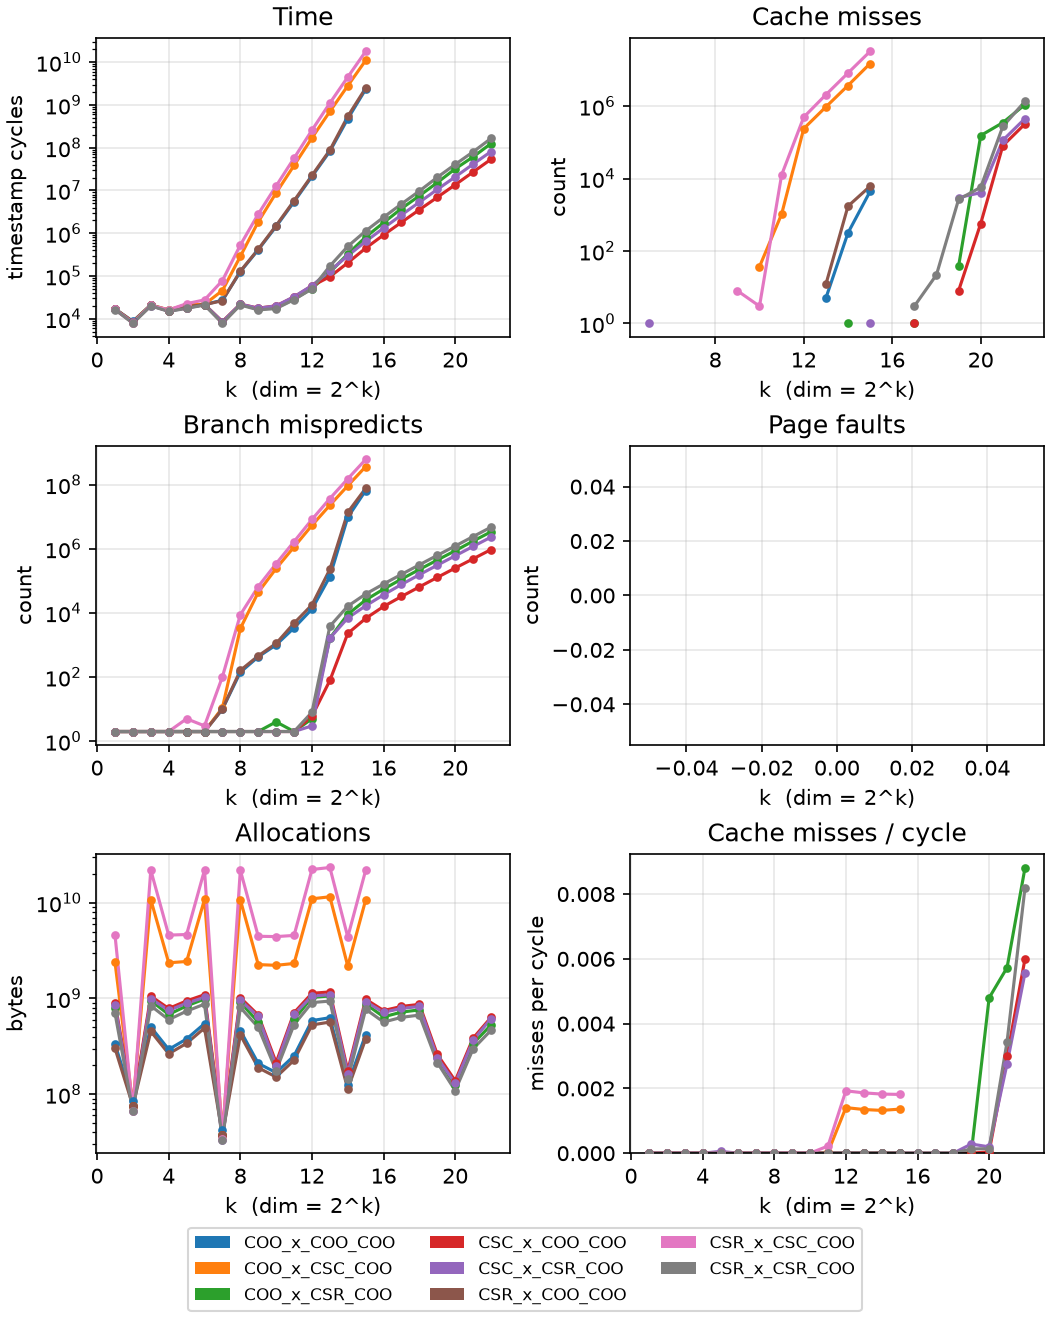
\includegraphics[width=0.85\linewidth,height=0.75\textheight,keepaspectratio]{figures/formats_ATP-GR-QC_s2.png}
    \caption{ATP-GR-QC Sample 2 comparison.}
    \label{fig:formats_ATP-GR-QC}
\end{figure}

\begin{figure}[htbp]
    \centering
    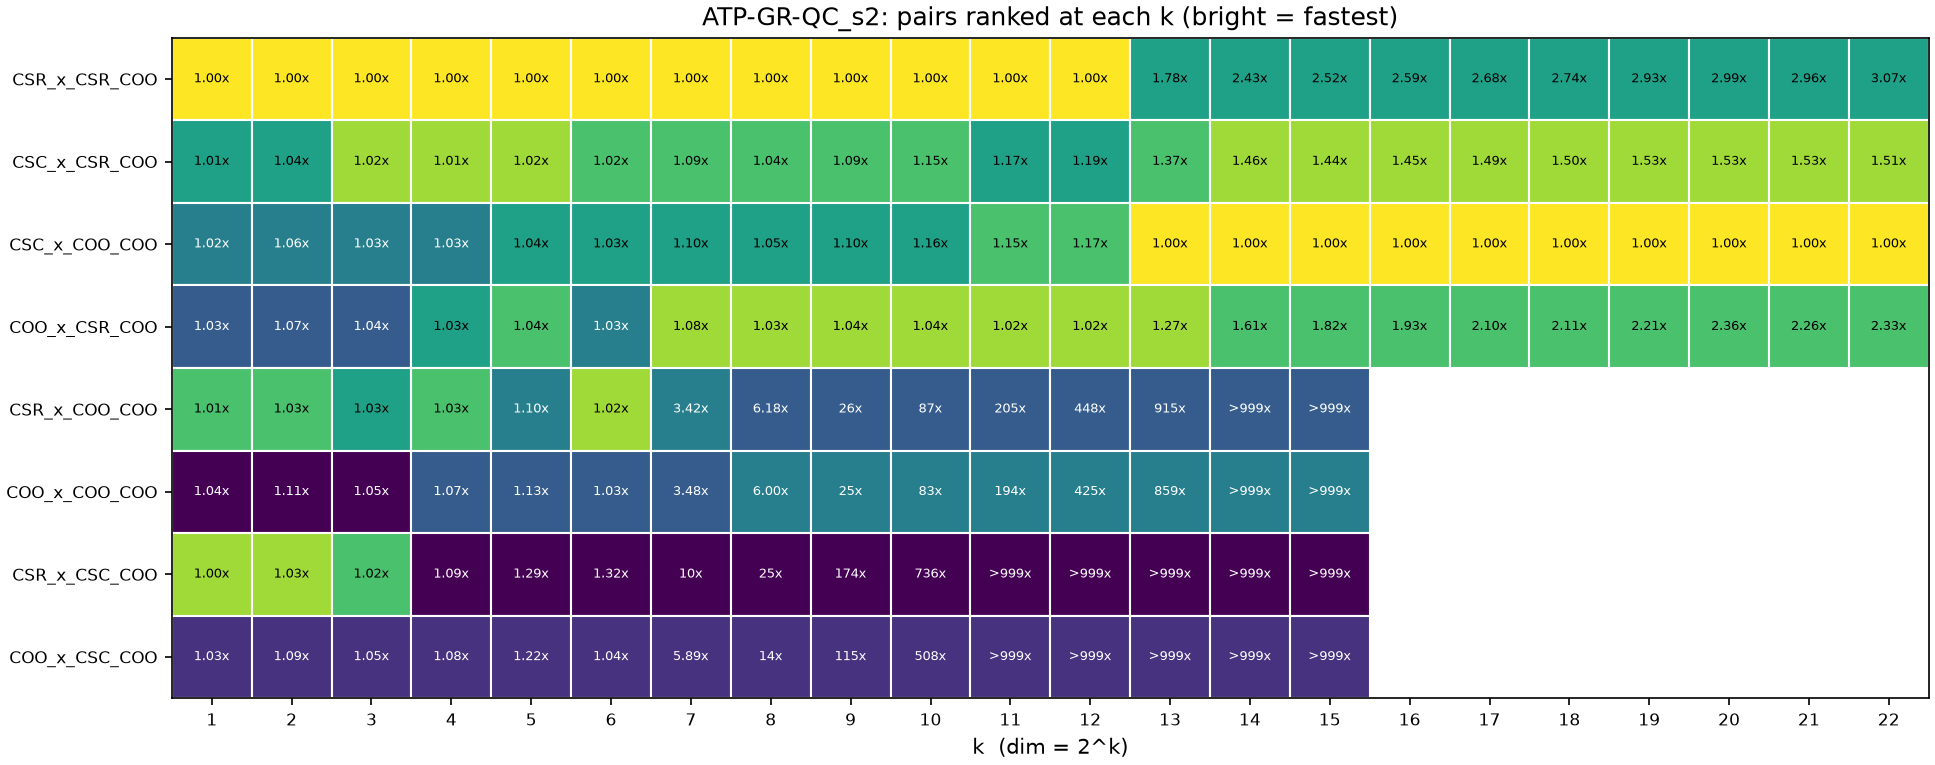
\includegraphics[width=\linewidth,height=0.6\textheight,keepaspectratio]{figures/formats_ranks_ATP-GR-QC_s2.png}
    \caption{ATP-GR-QC Sample 2: format pairs ranked at each $k$. Brighter cells are faster; each number is the slowdown relative to the fastest pair at that $k$.}
    \label{fig:formats_ranks_ATP-GR-QC}
\end{figure}
\clearpage

\begin{figure}[htbp]
    \centering
    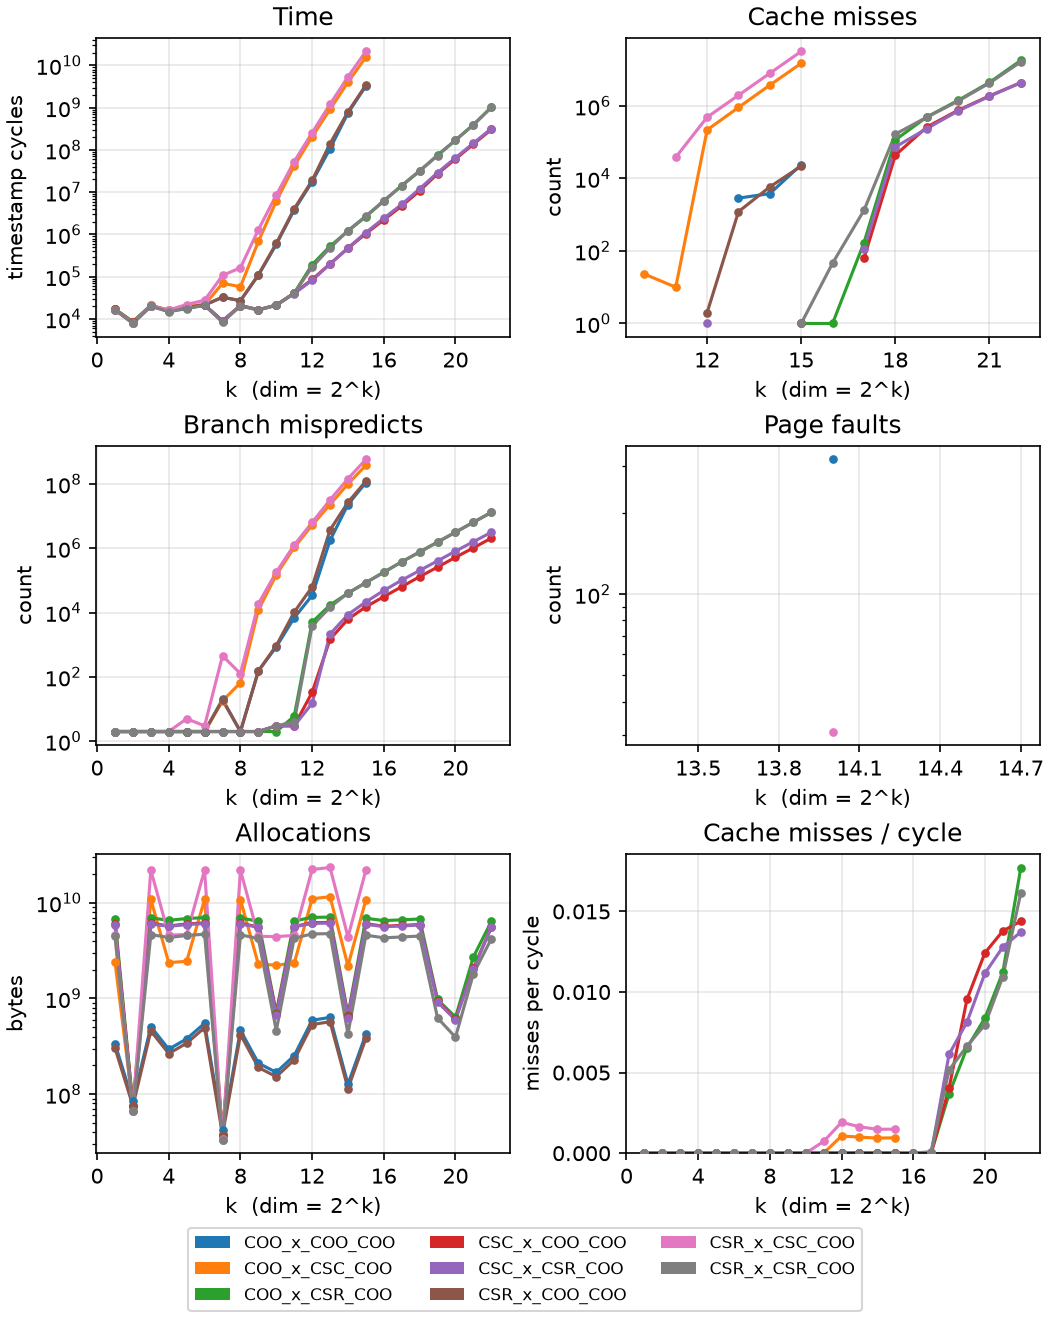
\includegraphics[width=0.85\linewidth,height=0.75\textheight,keepaspectratio]{figures/formats_Answers_s2.png}
    \caption{Answers Sample 2 comparison.}
    \label{fig:formats_Answers}
\end{figure}

\begin{figure}[htbp]
    \centering
    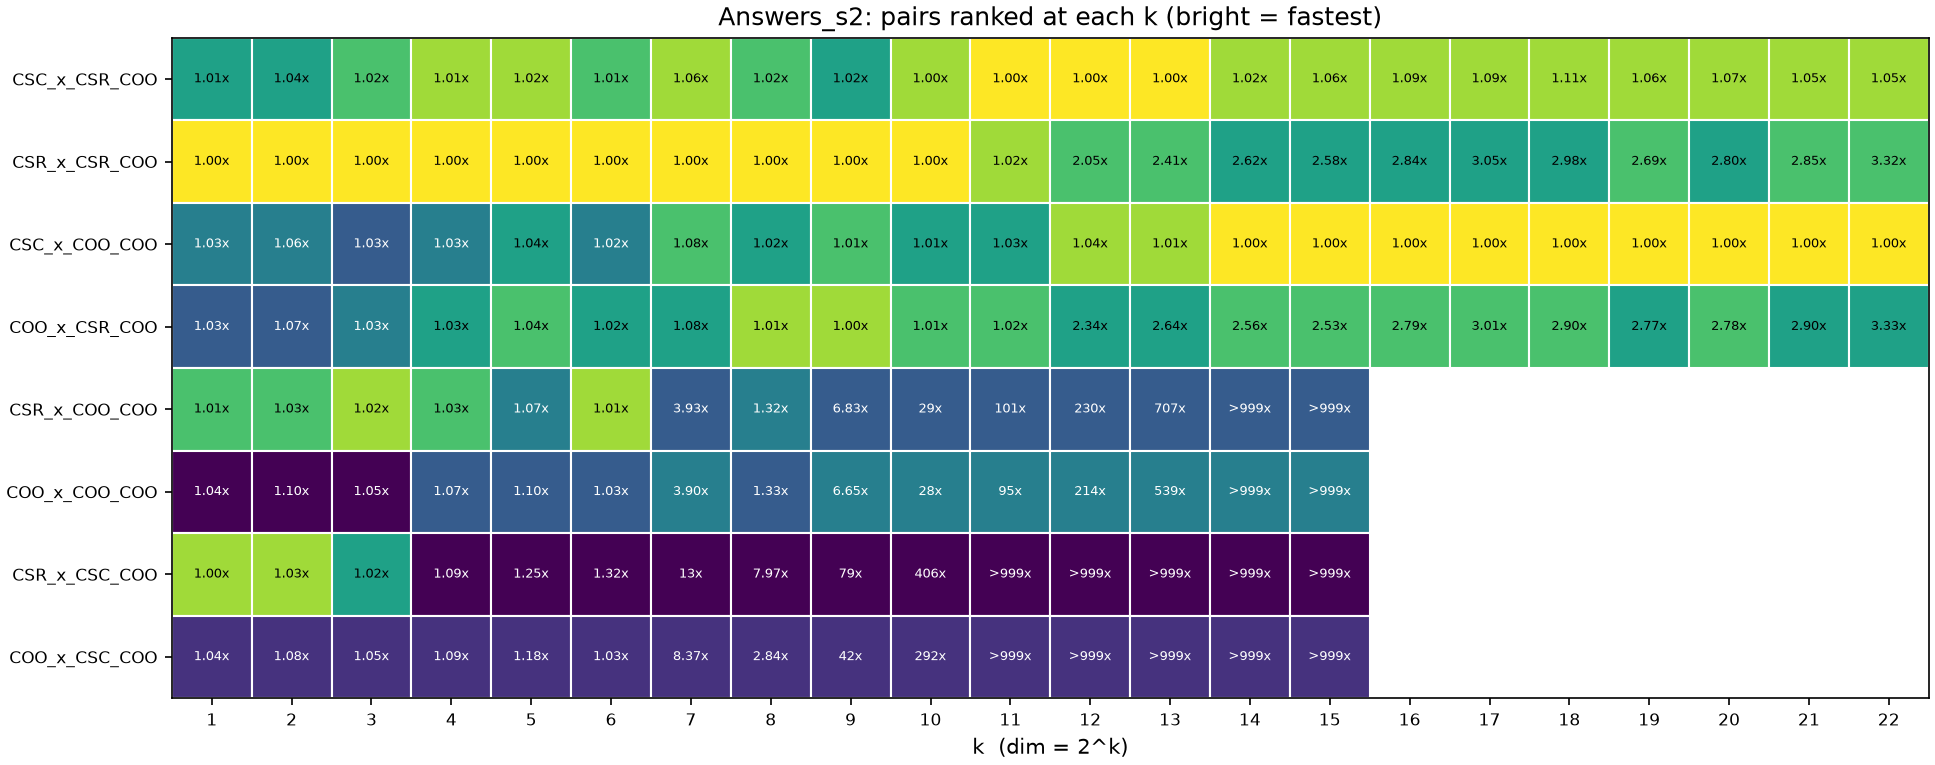
\includegraphics[width=\linewidth,height=0.6\textheight,keepaspectratio]{figures/formats_ranks_Answers_s2.png}
    \caption{Answers Sample 2: format pairs ranked at each $k$. Brighter cells are faster; each number is the slowdown relative to the fastest pair at that $k$.}
    \label{fig:formats_ranks_Answers}
\end{figure}
\clearpage

\begin{figure}[htbp]
    \centering
    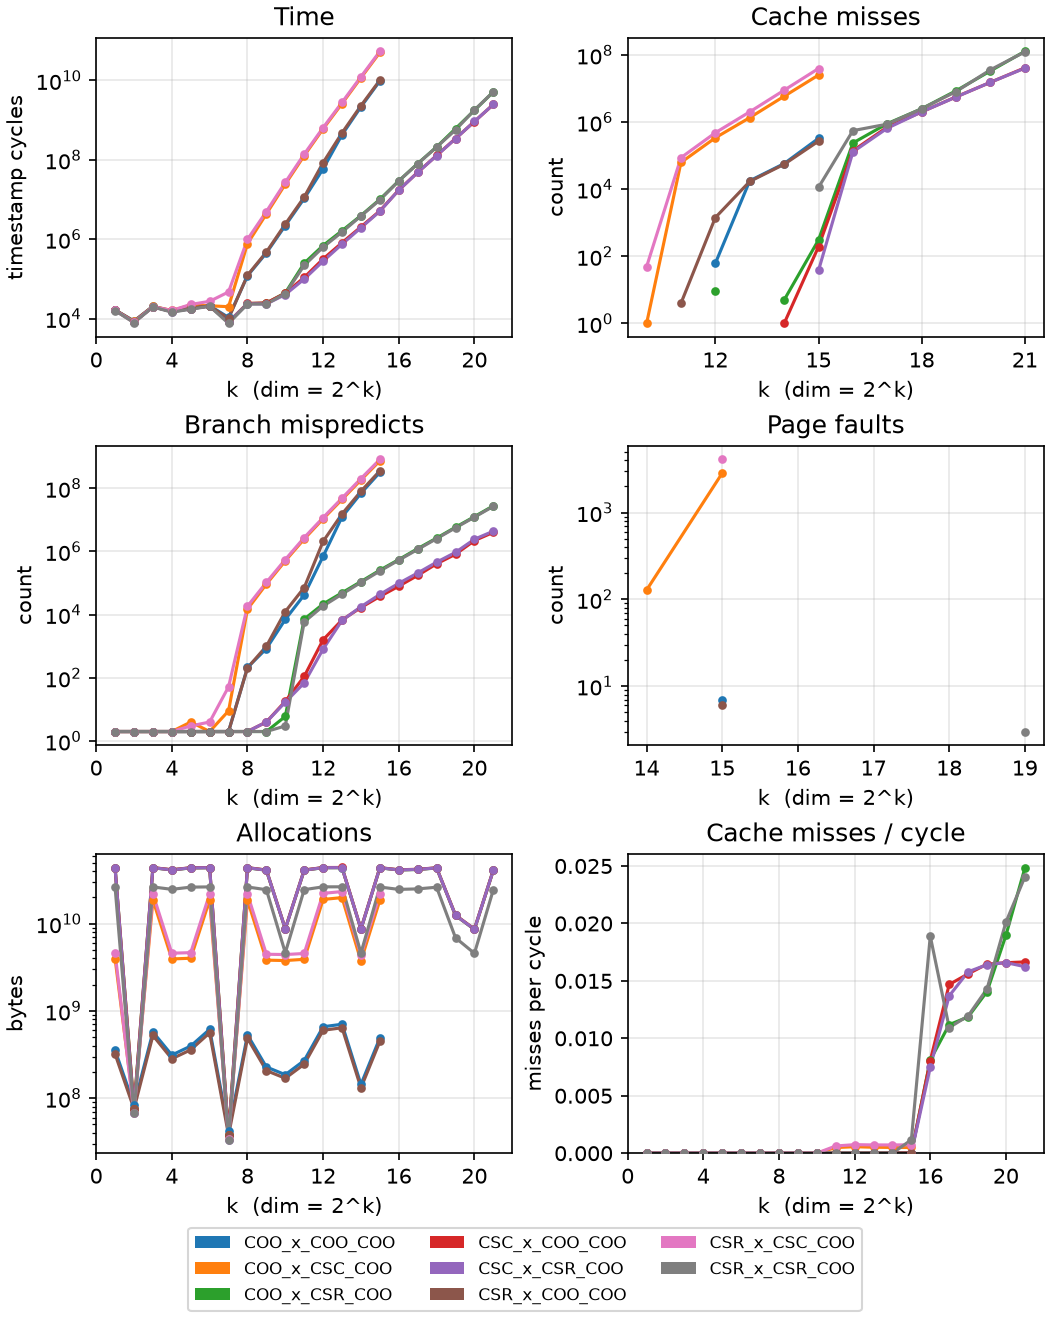
\includegraphics[width=0.85\linewidth,height=0.75\textheight,keepaspectratio]{figures/formats_Bio-Proteins_s2.png}
    \caption{Bio-Proteins Sample 2 comparison.}
    \label{fig:formats_Bio-Proteins}
\end{figure}

\begin{figure}[htbp]
    \centering
    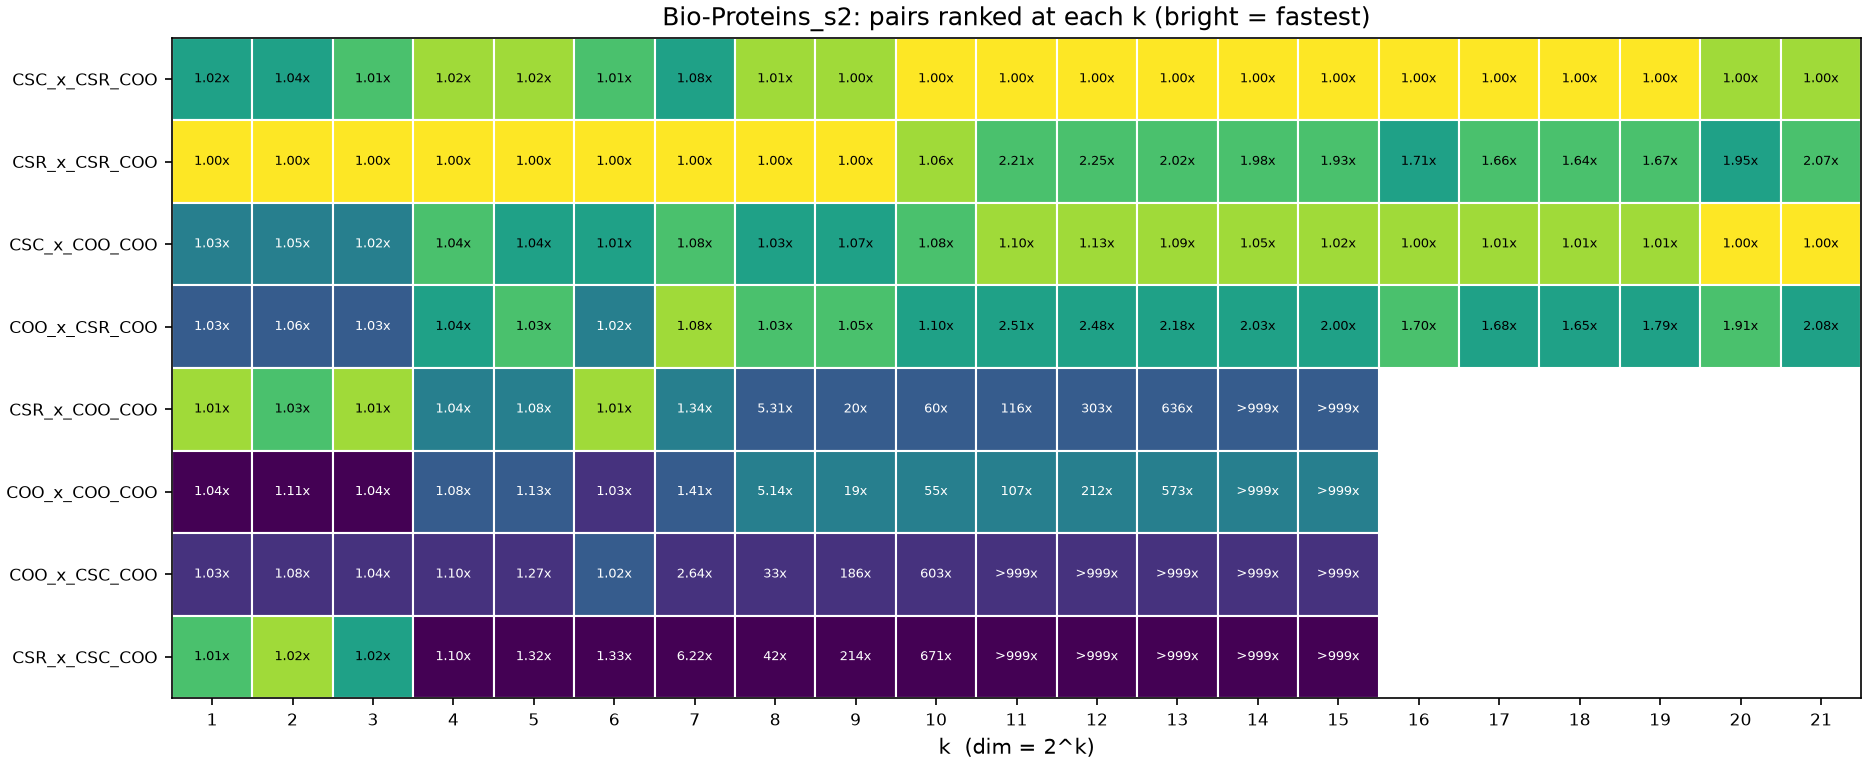
\includegraphics[width=\linewidth,height=0.6\textheight,keepaspectratio]{figures/formats_ranks_Bio-Proteins_s2.png}
    \caption{Bio-Proteins Sample 2: format pairs ranked at each $k$. Brighter cells are faster; each number is the slowdown relative to the fastest pair at that $k$.}
    \label{fig:formats_ranks_Bio-Proteins}
\end{figure}
\clearpage

\begin{figure}[htbp]
    \centering
    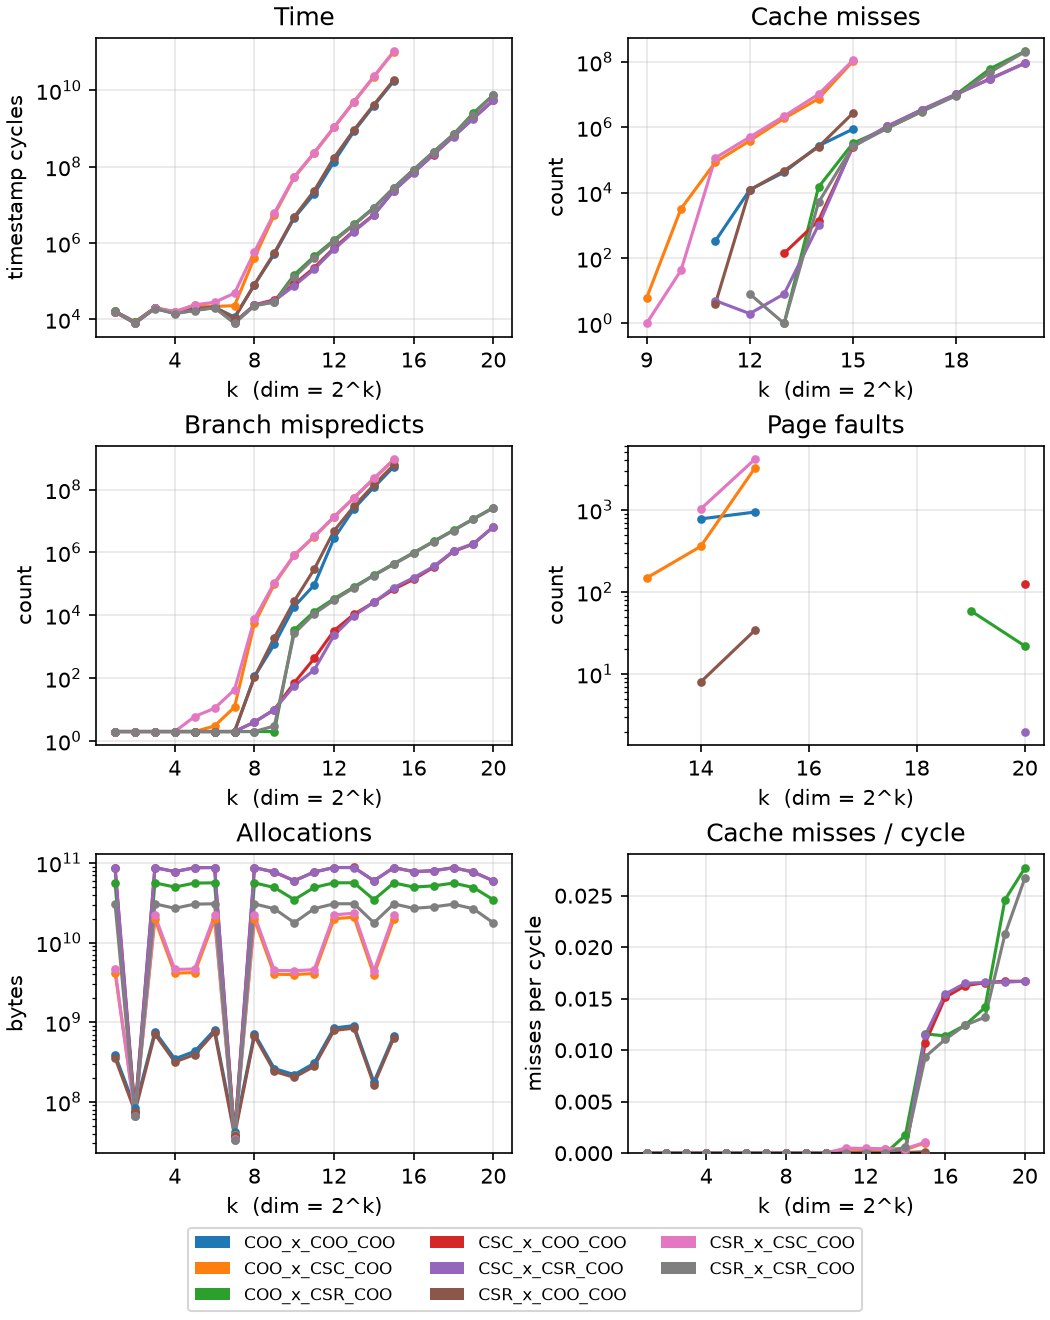
\includegraphics[width=0.85\linewidth,height=0.75\textheight,keepaspectratio]{figures/formats_Blog-Nat05-6m_s2.png}
    \caption{Blog-Nat05-6m Sample 2 comparison.}
    \label{fig:formats_Blog-Nat05-6m}
\end{figure}

\begin{figure}[htbp]
    \centering
    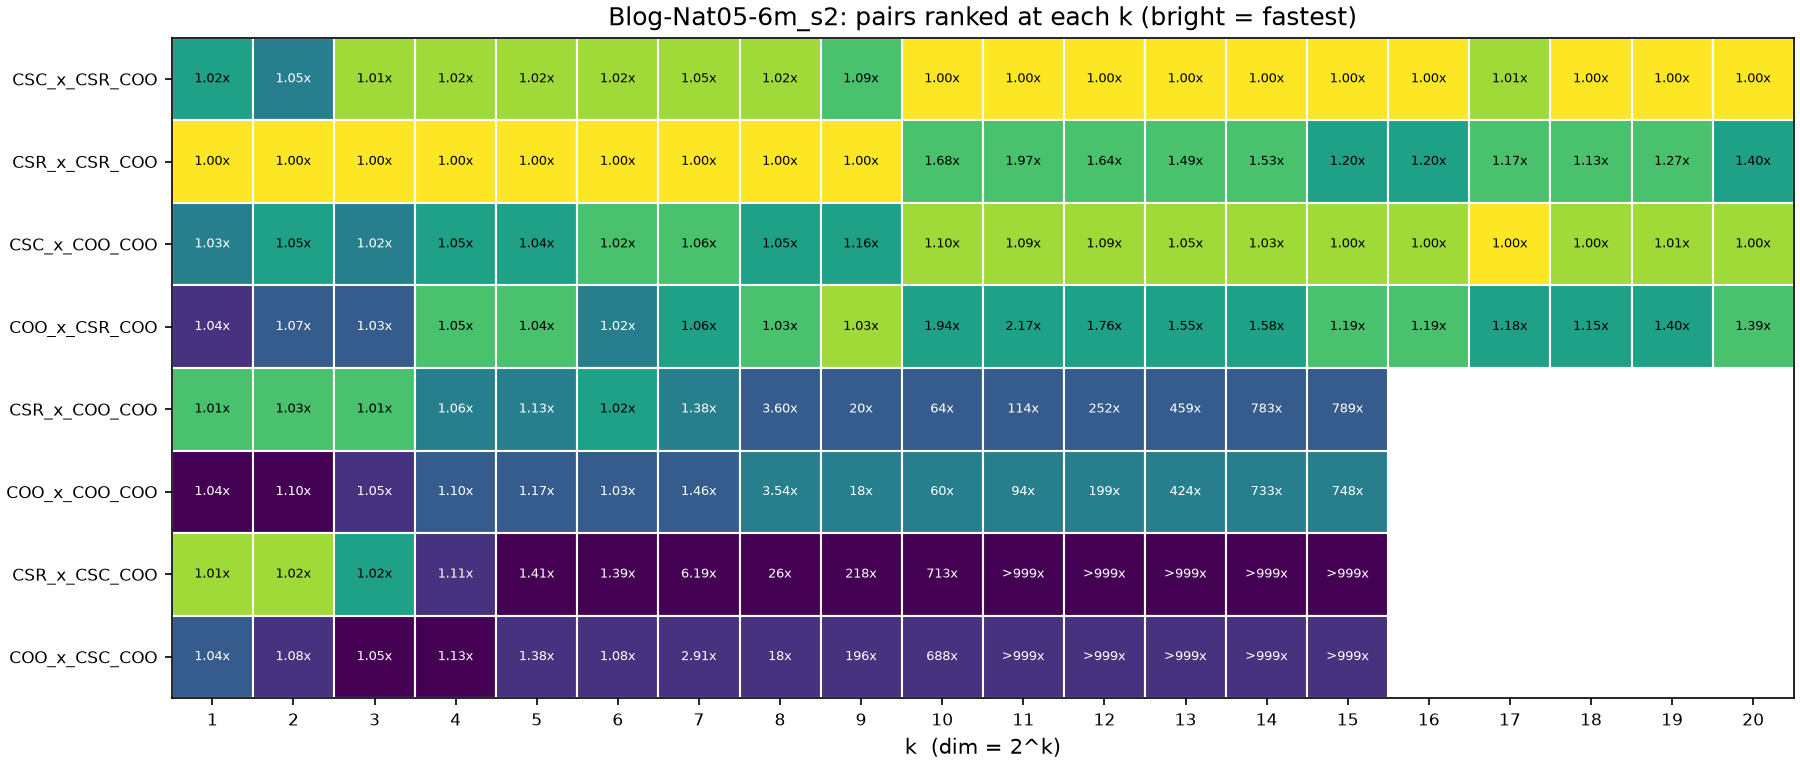
\includegraphics[width=\linewidth,height=0.6\textheight,keepaspectratio]{figures/formats_ranks_Blog-Nat05-6m_s2.png}
    \caption{Blog-Nat05-6m Sample 2: format pairs ranked at each $k$. Brighter cells are faster; each number is the slowdown relative to the fastest pair at that $k$.}
    \label{fig:formats_ranks_Blog-Nat05-6m}
\end{figure}
\clearpage

\begin{figure}[htbp]
    \centering
    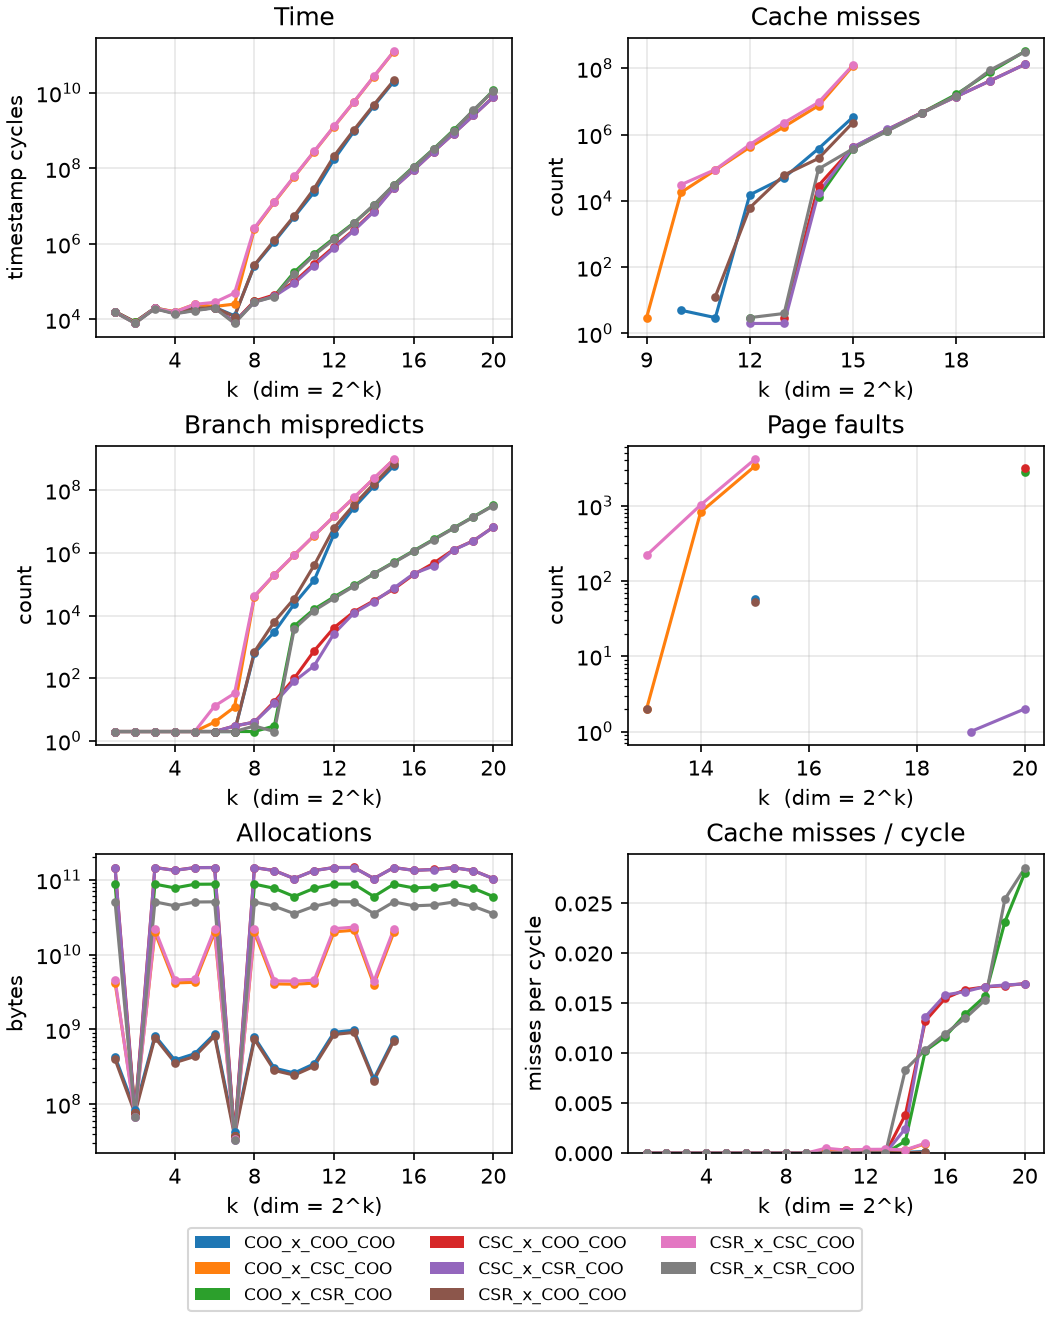
\includegraphics[width=0.85\linewidth,height=0.75\textheight,keepaspectratio]{figures/formats_Blog-Nat06all_s2.png}
    \caption{Blog-Nat06all Sample 2 comparison.}
    \label{fig:formats_Blog-Nat06all}
\end{figure}

\begin{figure}[htbp]
    \centering
    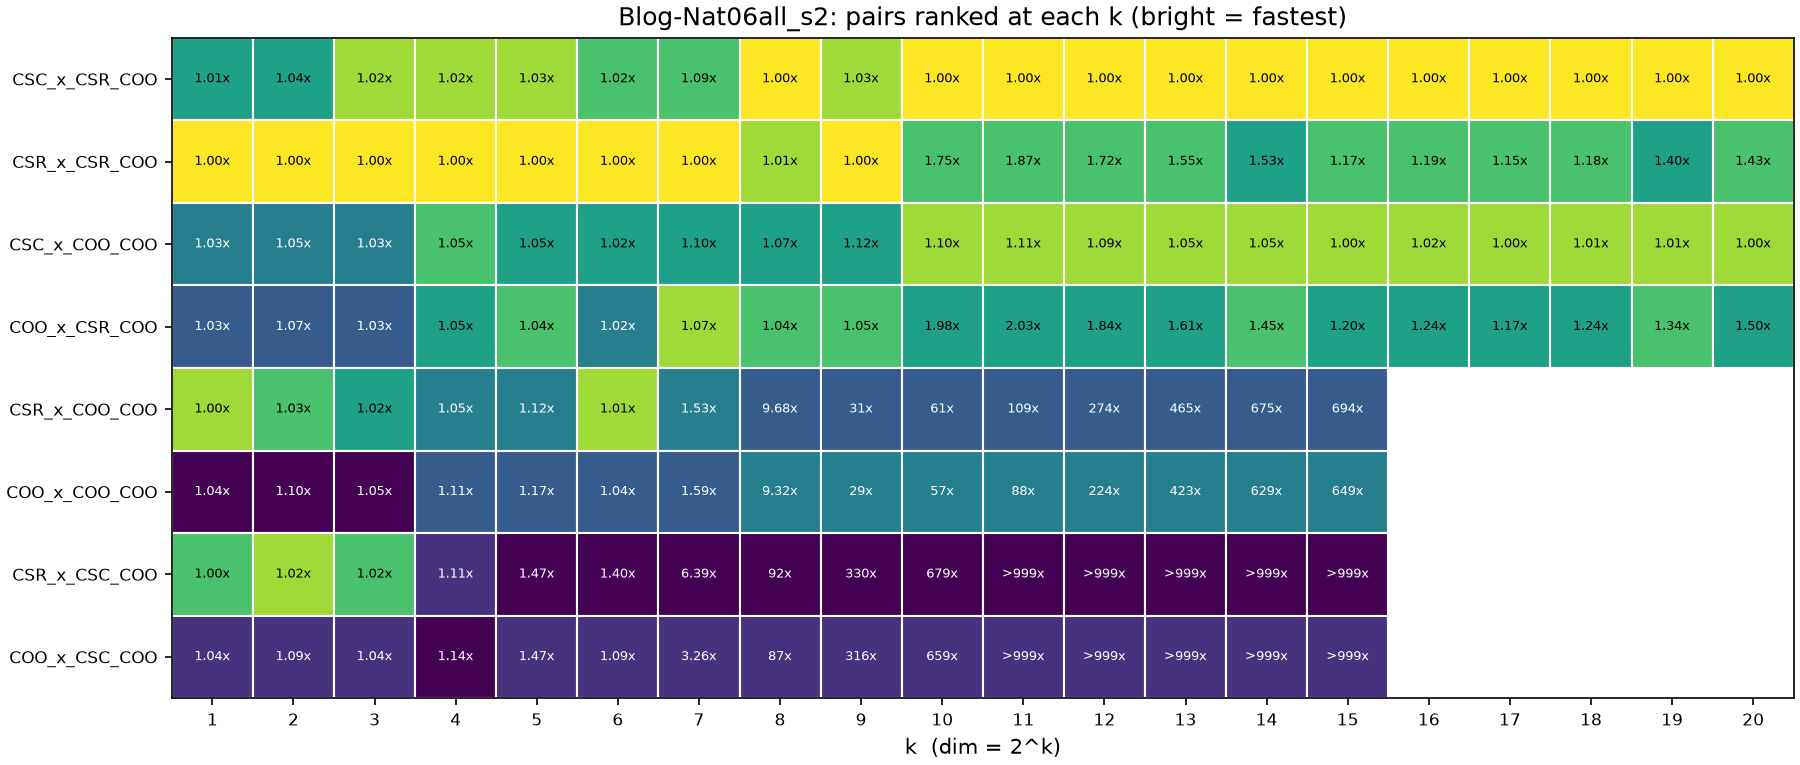
\includegraphics[width=\linewidth,height=0.6\textheight,keepaspectratio]{figures/formats_ranks_Blog-Nat06all_s2.png}
    \caption{Blog-Nat06all Sample 2: format pairs ranked at each $k$. Brighter cells are faster; each number is the slowdown relative to the fastest pair at that $k$.}
    \label{fig:formats_ranks_Blog-Nat06all}
\end{figure}
\clearpage

\begin{figure}[htbp]
    \centering
    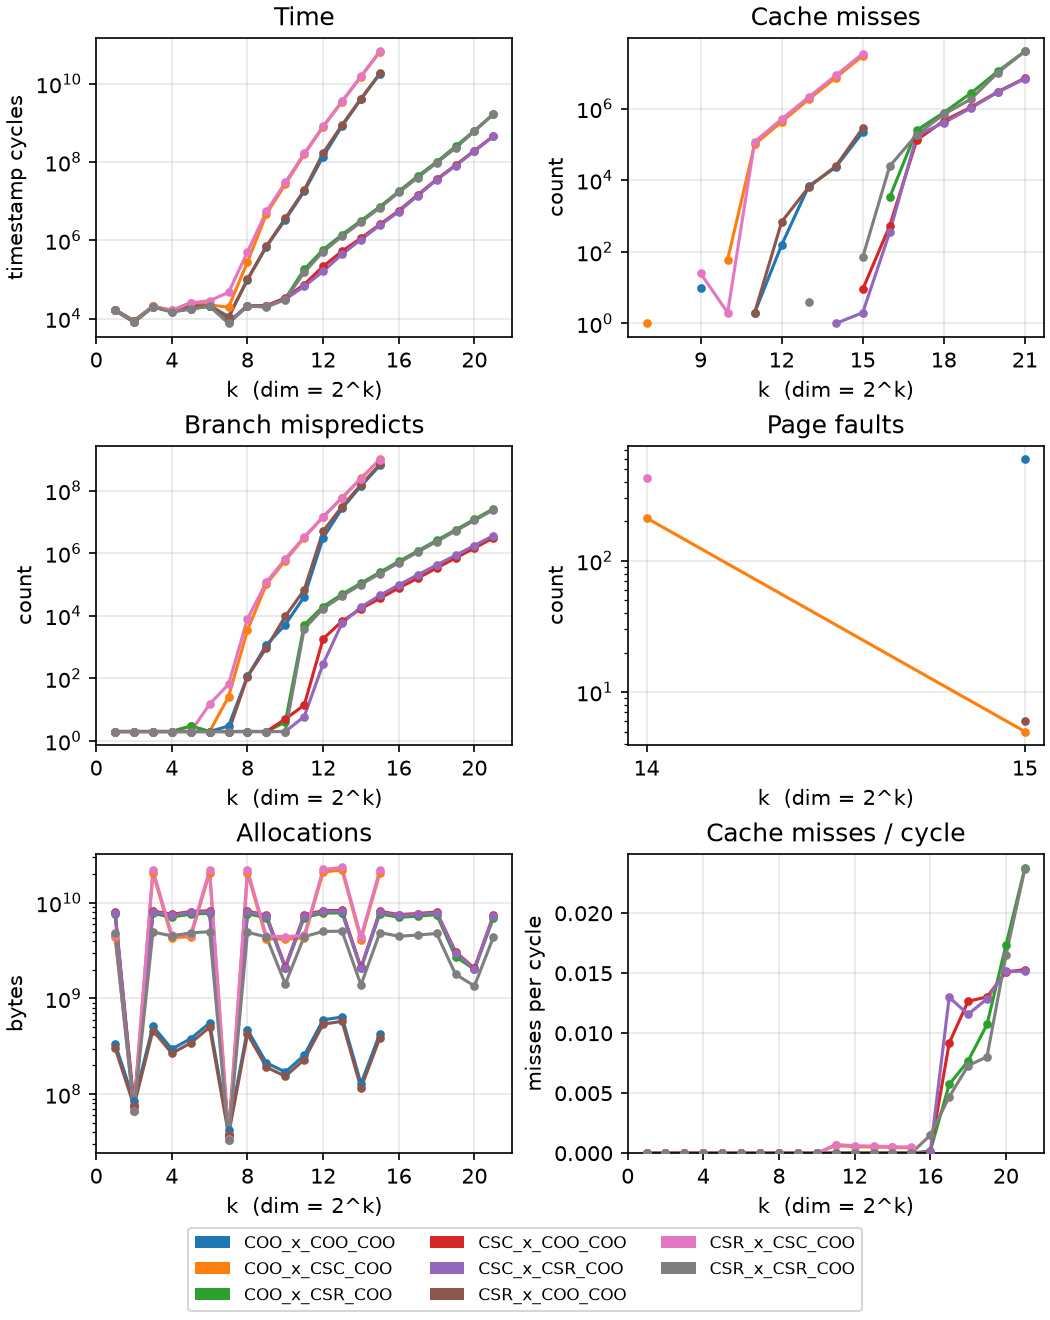
\includegraphics[width=0.85\linewidth,height=0.75\textheight,keepaspectratio]{figures/formats_CA-DBLP_s2.png}
    \caption{CA-DBLP Sample 2 comparison.}
    \label{fig:formats_CA-DBLP}
\end{figure}

\begin{figure}[htbp]
    \centering
    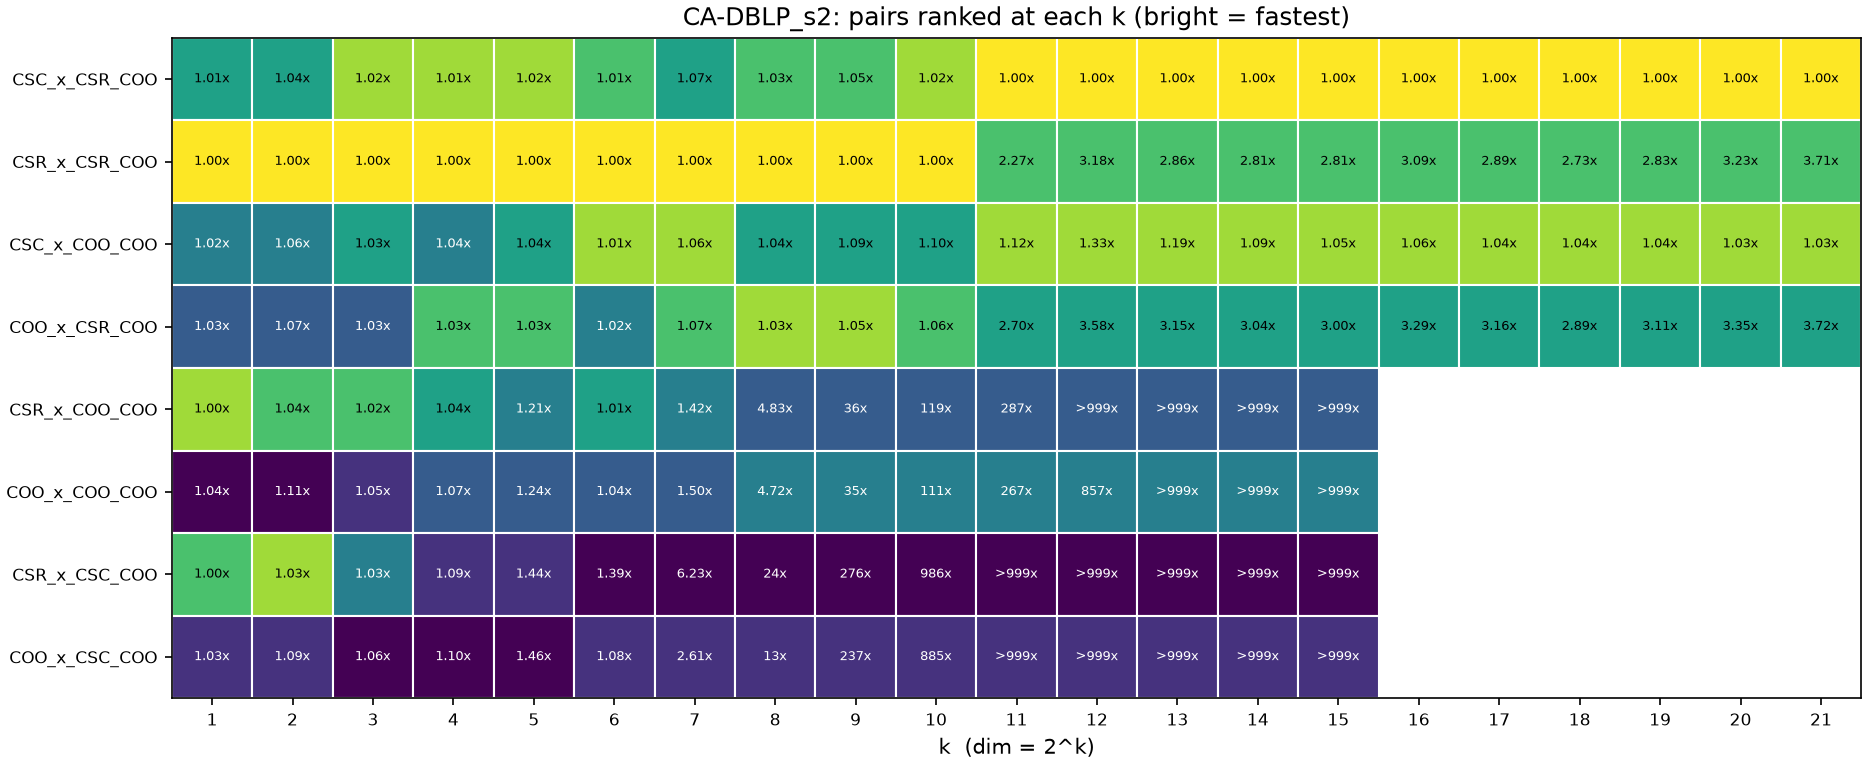
\includegraphics[width=\linewidth,height=0.6\textheight,keepaspectratio]{figures/formats_ranks_CA-DBLP_s2.png}
    \caption{CA-DBLP Sample 2: format pairs ranked at each $k$. Brighter cells are faster; each number is the slowdown relative to the fastest pair at that $k$.}
    \label{fig:formats_ranks_CA-DBLP}
\end{figure}
\clearpage

\begin{figure}[htbp]
    \centering
    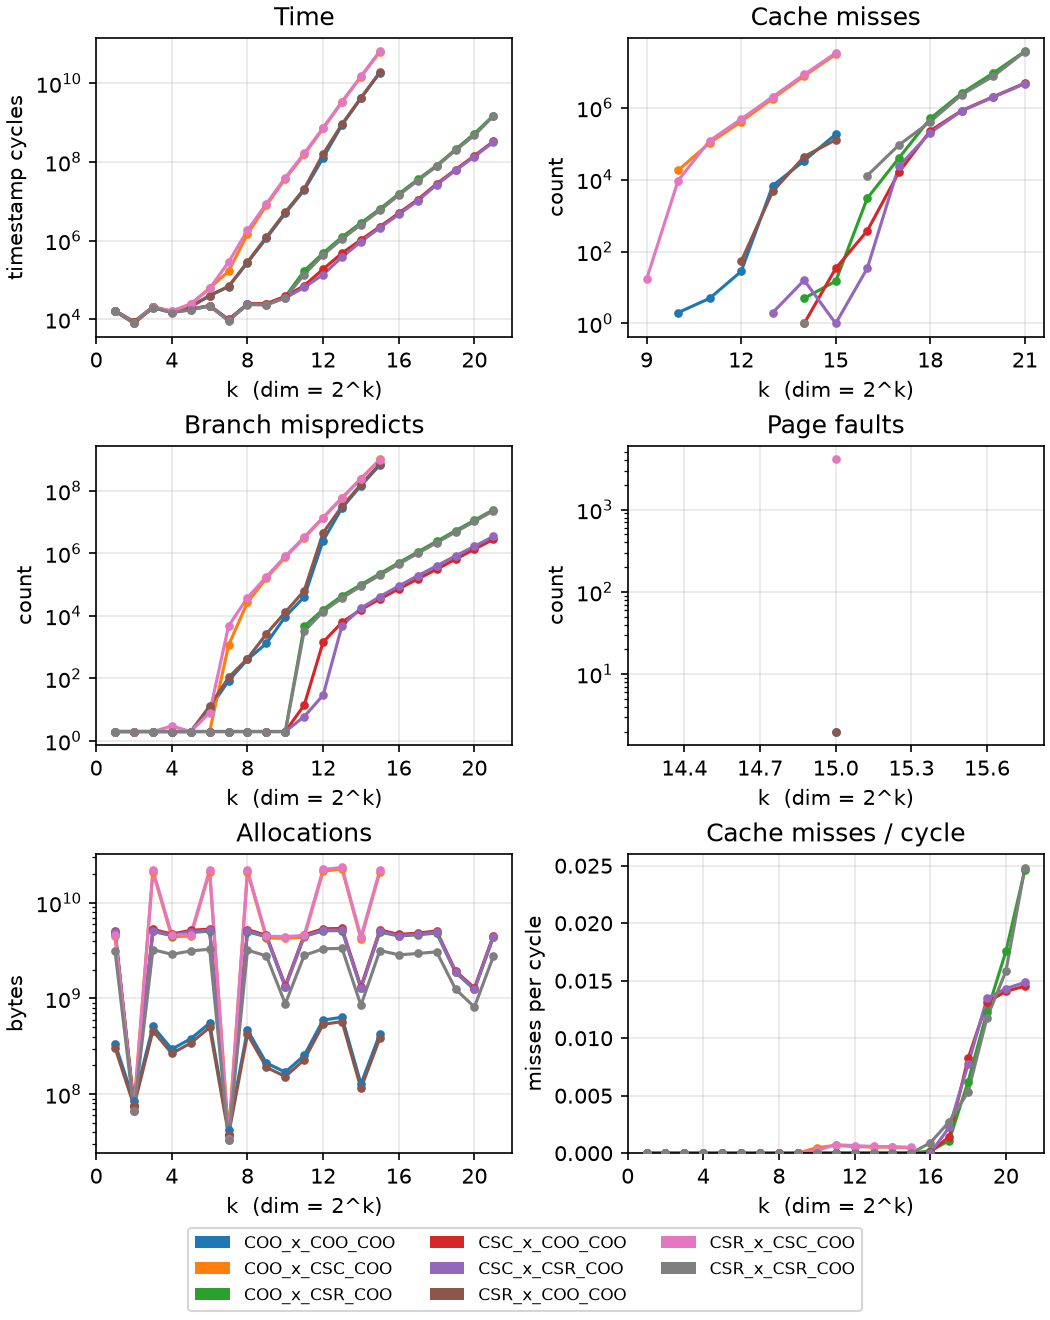
\includegraphics[width=0.85\linewidth,height=0.75\textheight,keepaspectratio]{figures/formats_CA-GR-QC_s2.png}
    \caption{CA-GR-QC Sample 2 comparison.}
    \label{fig:formats_CA-GR-QC}
\end{figure}

\begin{figure}[htbp]
    \centering
    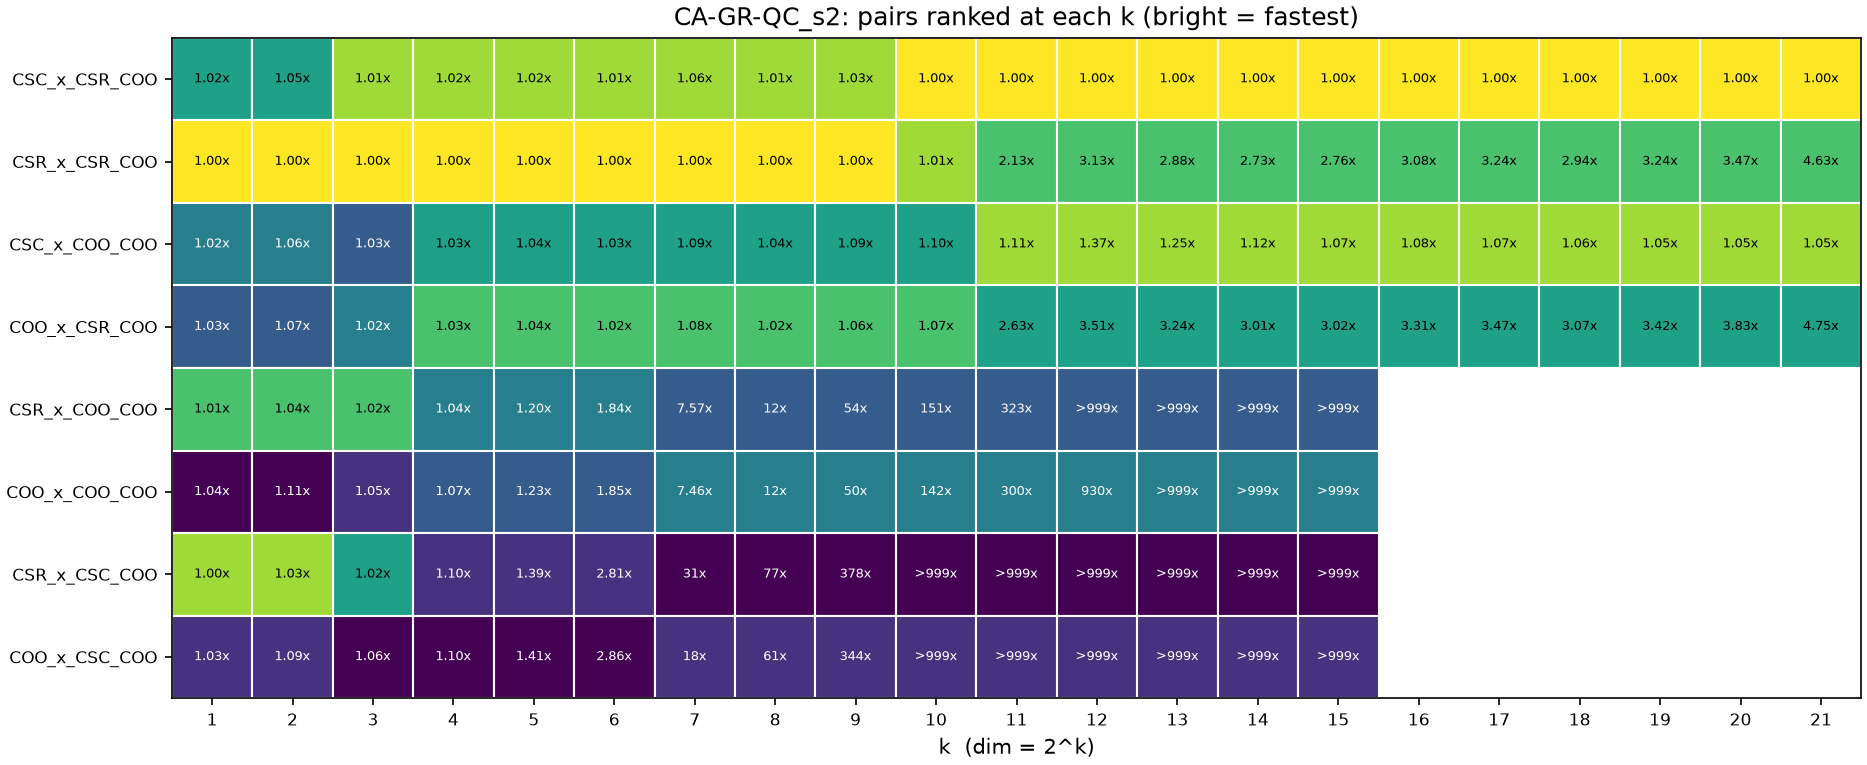
\includegraphics[width=\linewidth,height=0.6\textheight,keepaspectratio]{figures/formats_ranks_CA-GR-QC_s2.png}
    \caption{CA-GR-QC Sample 2: format pairs ranked at each $k$. Brighter cells are faster; each number is the slowdown relative to the fastest pair at that $k$.}
    \label{fig:formats_ranks_CA-GR-QC}
\end{figure}
\clearpage

\begin{figure}[htbp]
    \centering
    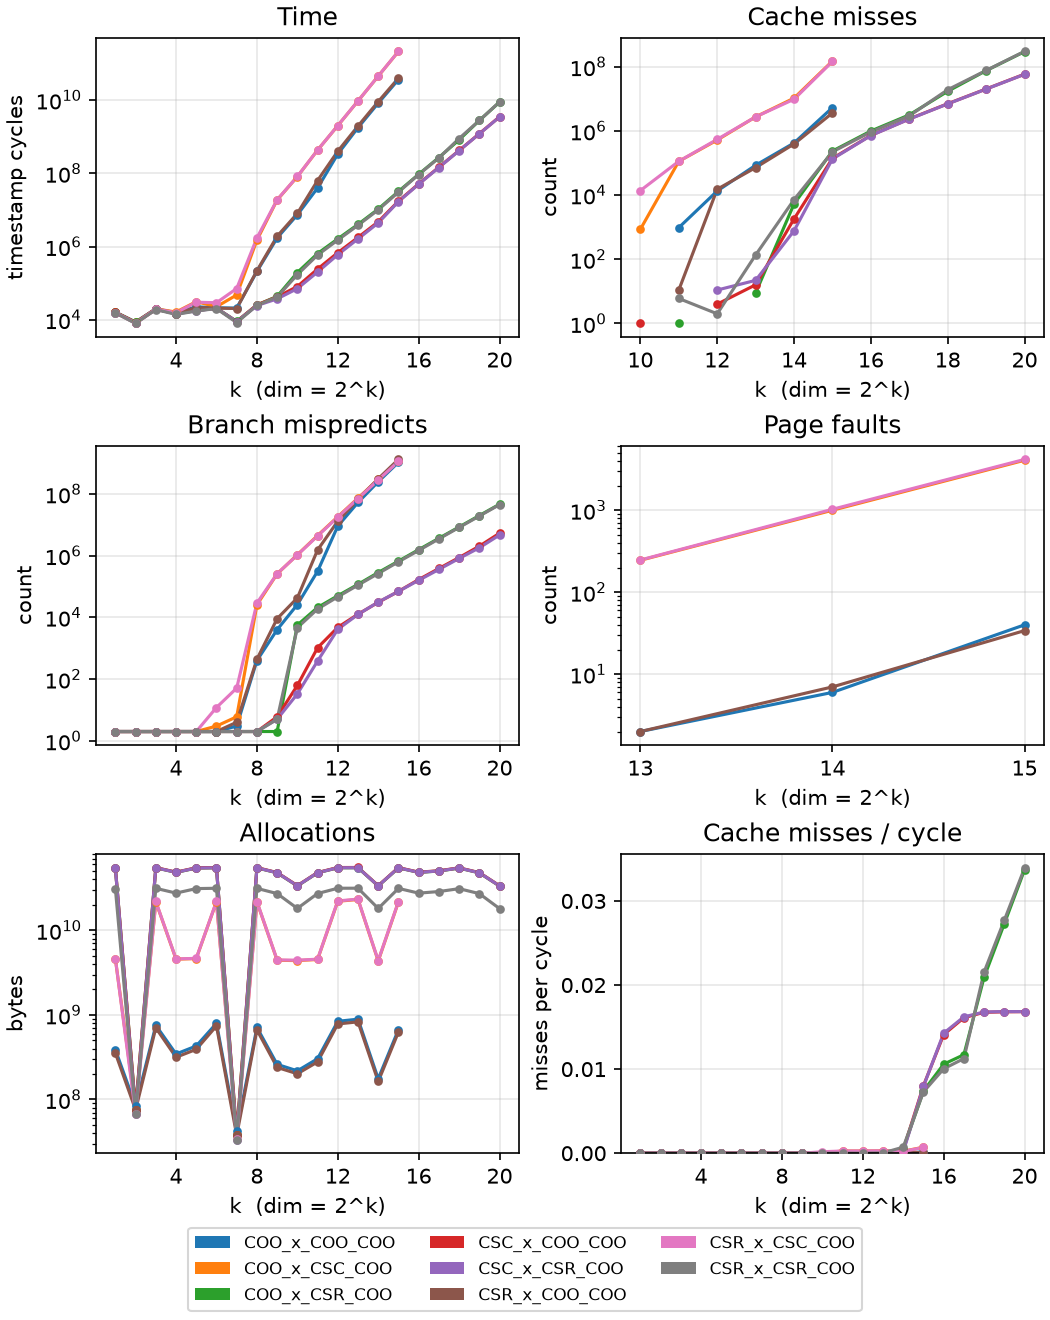
\includegraphics[width=0.85\linewidth,height=0.75\textheight,keepaspectratio]{figures/formats_CA-Hep-Ph_s2.png}
    \caption{CA-Hep-Ph Sample 2 comparison.}
    \label{fig:formats_CA-Hep-Ph}
\end{figure}

\begin{figure}[htbp]
    \centering
    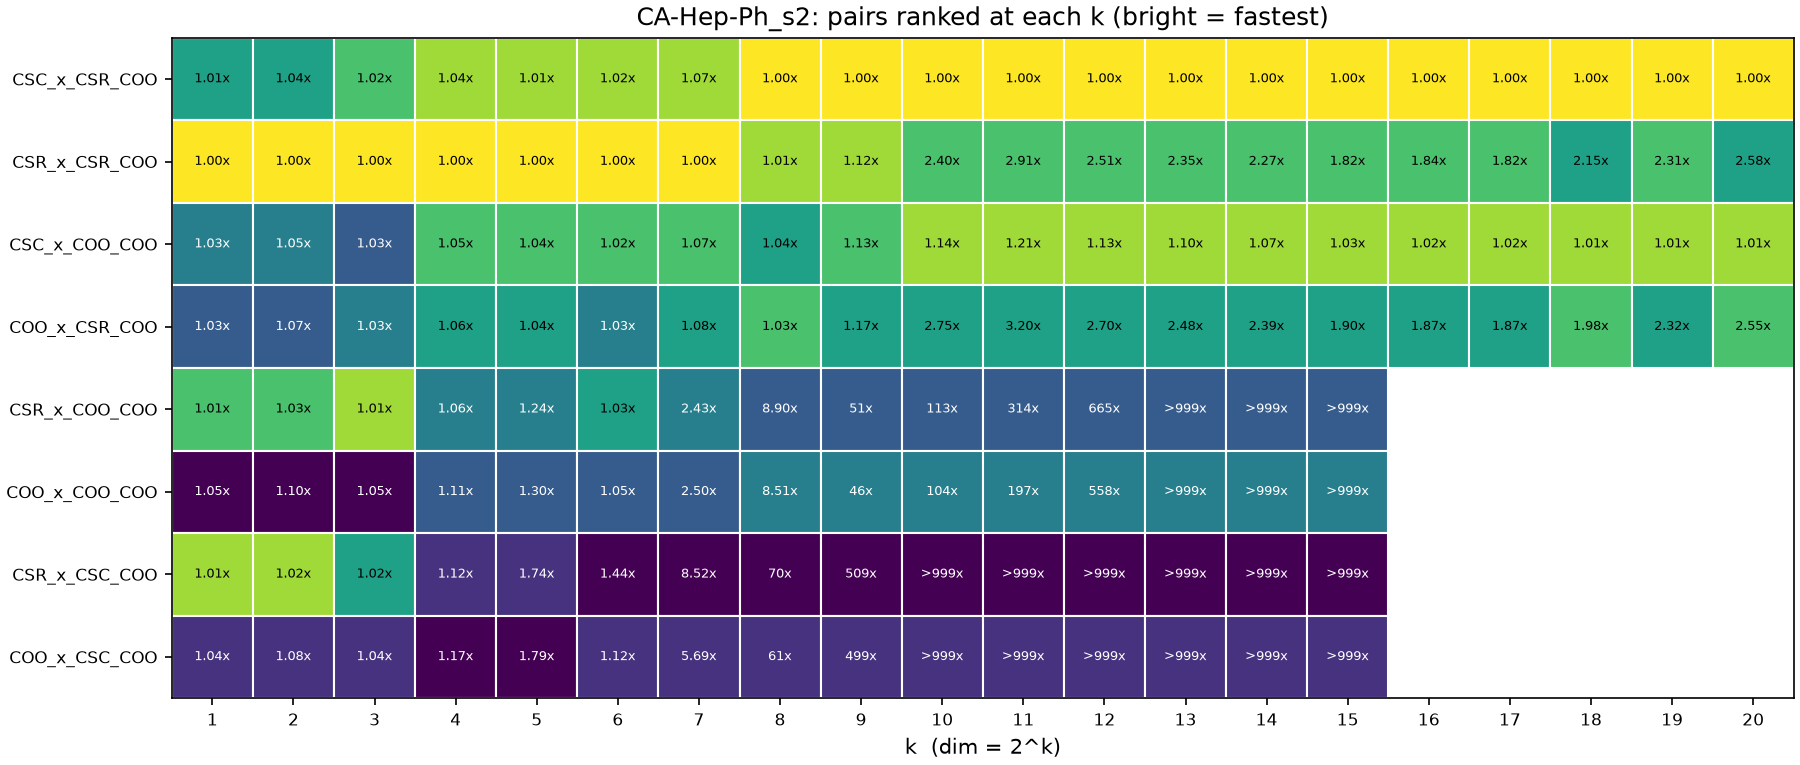
\includegraphics[width=\linewidth,height=0.6\textheight,keepaspectratio]{figures/formats_ranks_CA-Hep-Ph_s2.png}
    \caption{CA-Hep-Ph Sample 2: format pairs ranked at each $k$. Brighter cells are faster; each number is the slowdown relative to the fastest pair at that $k$.}
    \label{fig:formats_ranks_CA-Hep-Ph}
\end{figure}
\clearpage

\begin{figure}[htbp]
    \centering
    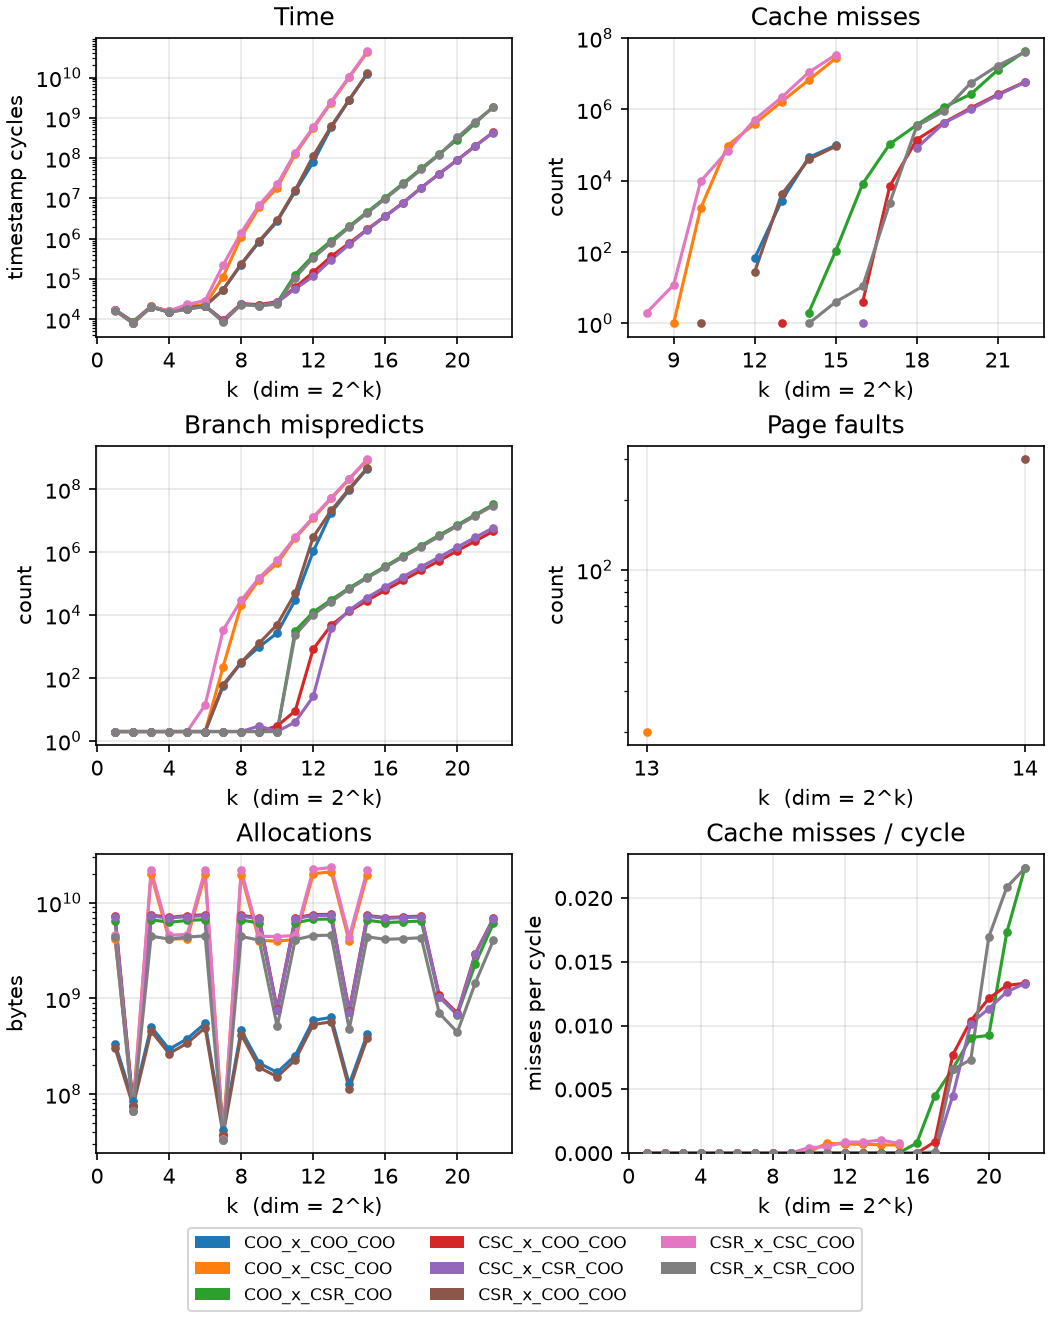
\includegraphics[width=0.85\linewidth,height=0.75\textheight,keepaspectratio]{figures/formats_CA-Hep-Th_s2.png}
    \caption{CA-Hep-Th Sample 2 comparison.}
    \label{fig:formats_CA-Hep-Th}
\end{figure}

\begin{figure}[htbp]
    \centering
    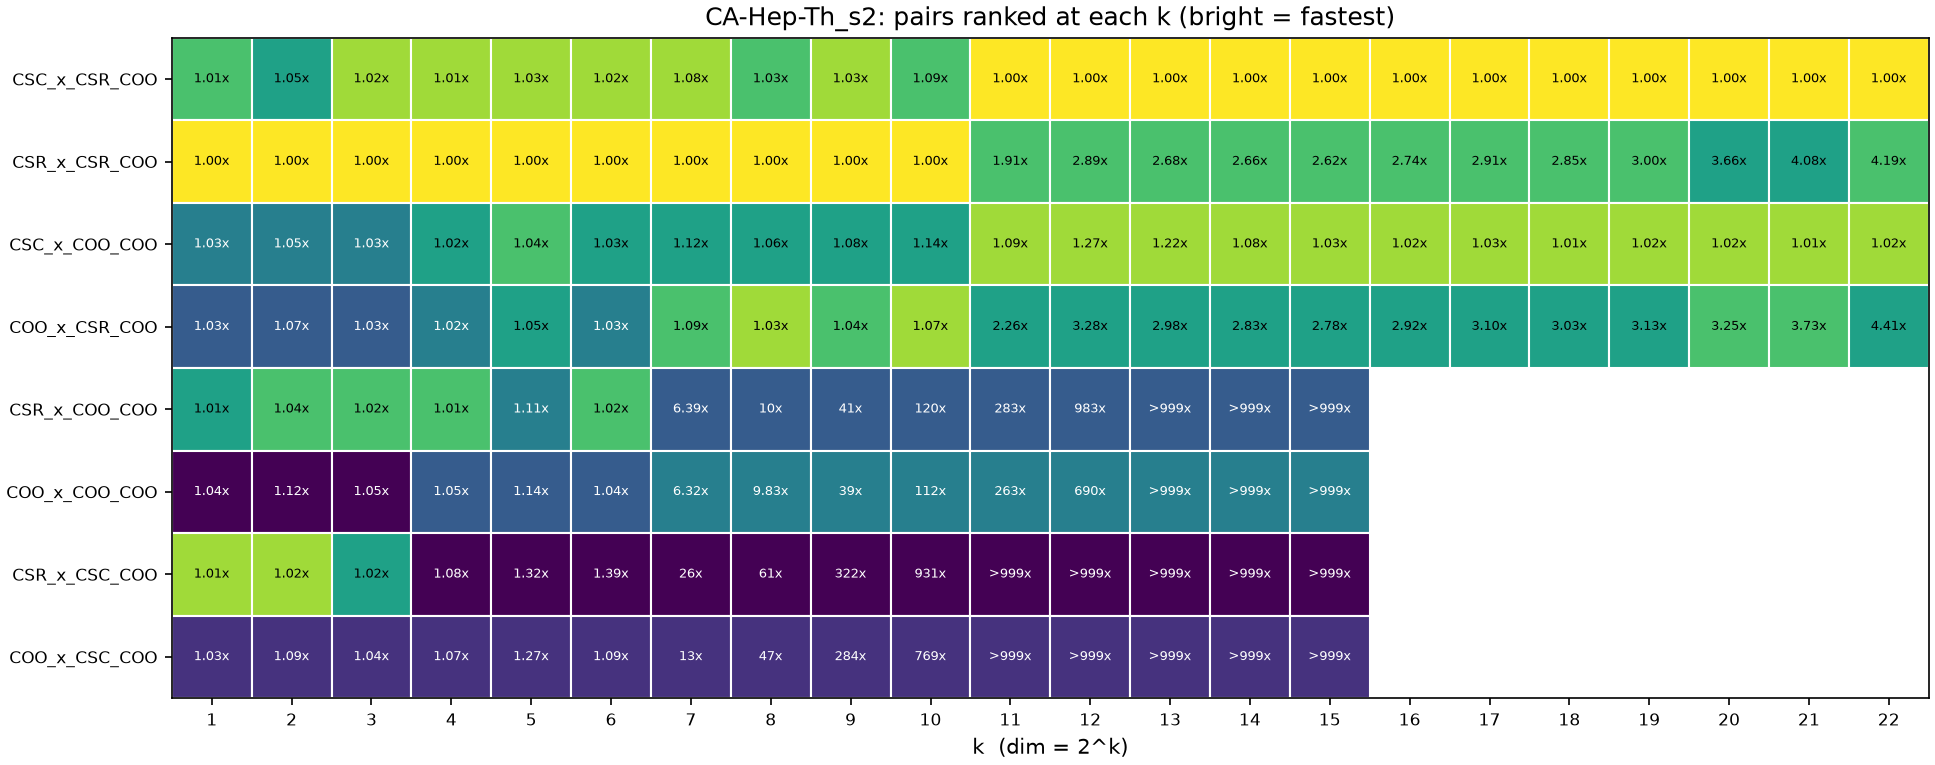
\includegraphics[width=\linewidth,height=0.6\textheight,keepaspectratio]{figures/formats_ranks_CA-Hep-Th_s2.png}
    \caption{CA-Hep-Th Sample 2: format pairs ranked at each $k$. Brighter cells are faster; each number is the slowdown relative to the fastest pair at that $k$.}
    \label{fig:formats_ranks_CA-Hep-Th}
\end{figure}
\clearpage

\begin{figure}[htbp]
    \centering
    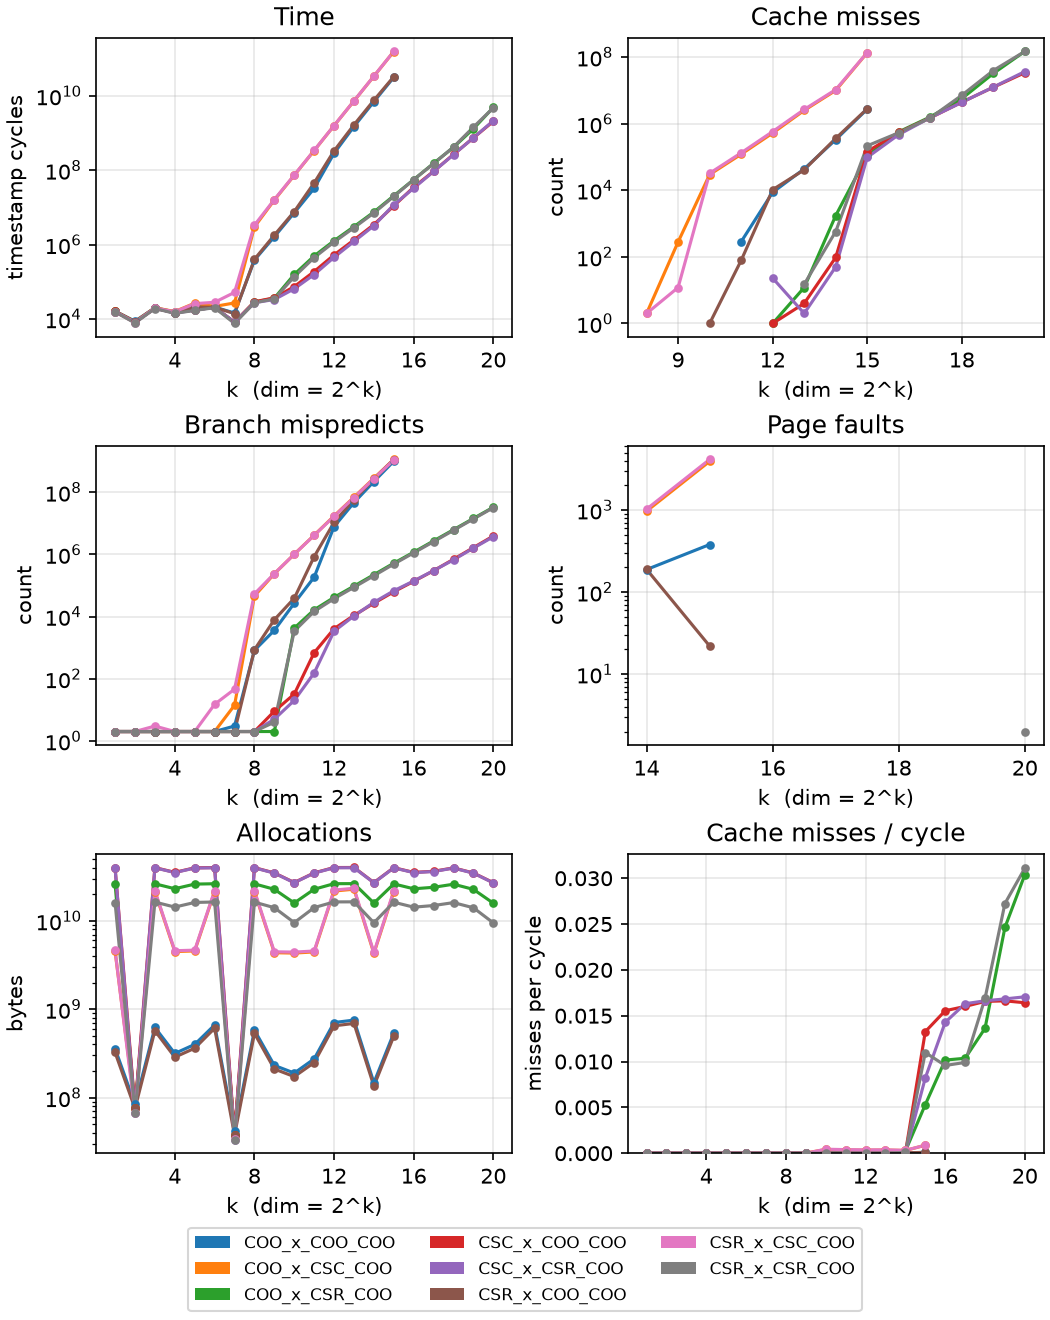
\includegraphics[width=0.85\linewidth,height=0.75\textheight,keepaspectratio]{figures/formats_Cit-Hep-Ph_s2.png}
    \caption{Cit-Hep-Ph Sample 2 comparison.}
    \label{fig:formats_Cit-Hep-Ph}
\end{figure}

\begin{figure}[htbp]
    \centering
    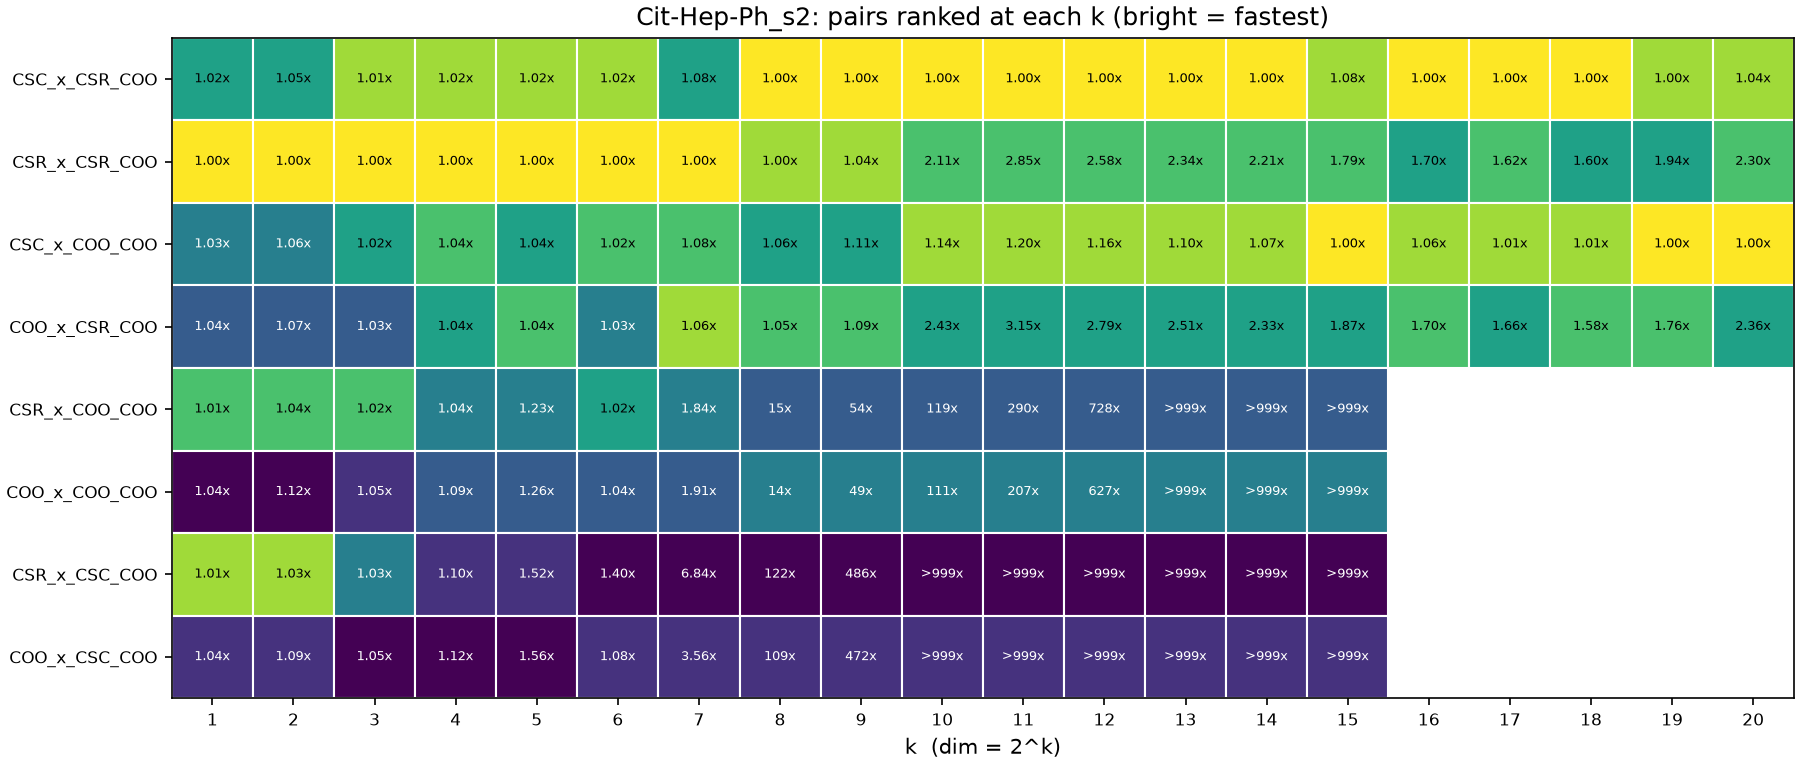
\includegraphics[width=\linewidth,height=0.6\textheight,keepaspectratio]{figures/formats_ranks_Cit-Hep-Ph_s2.png}
    \caption{Cit-Hep-Ph Sample 2: format pairs ranked at each $k$. Brighter cells are faster; each number is the slowdown relative to the fastest pair at that $k$.}
    \label{fig:formats_ranks_Cit-Hep-Ph}
\end{figure}
\clearpage

\begin{figure}[htbp]
    \centering
    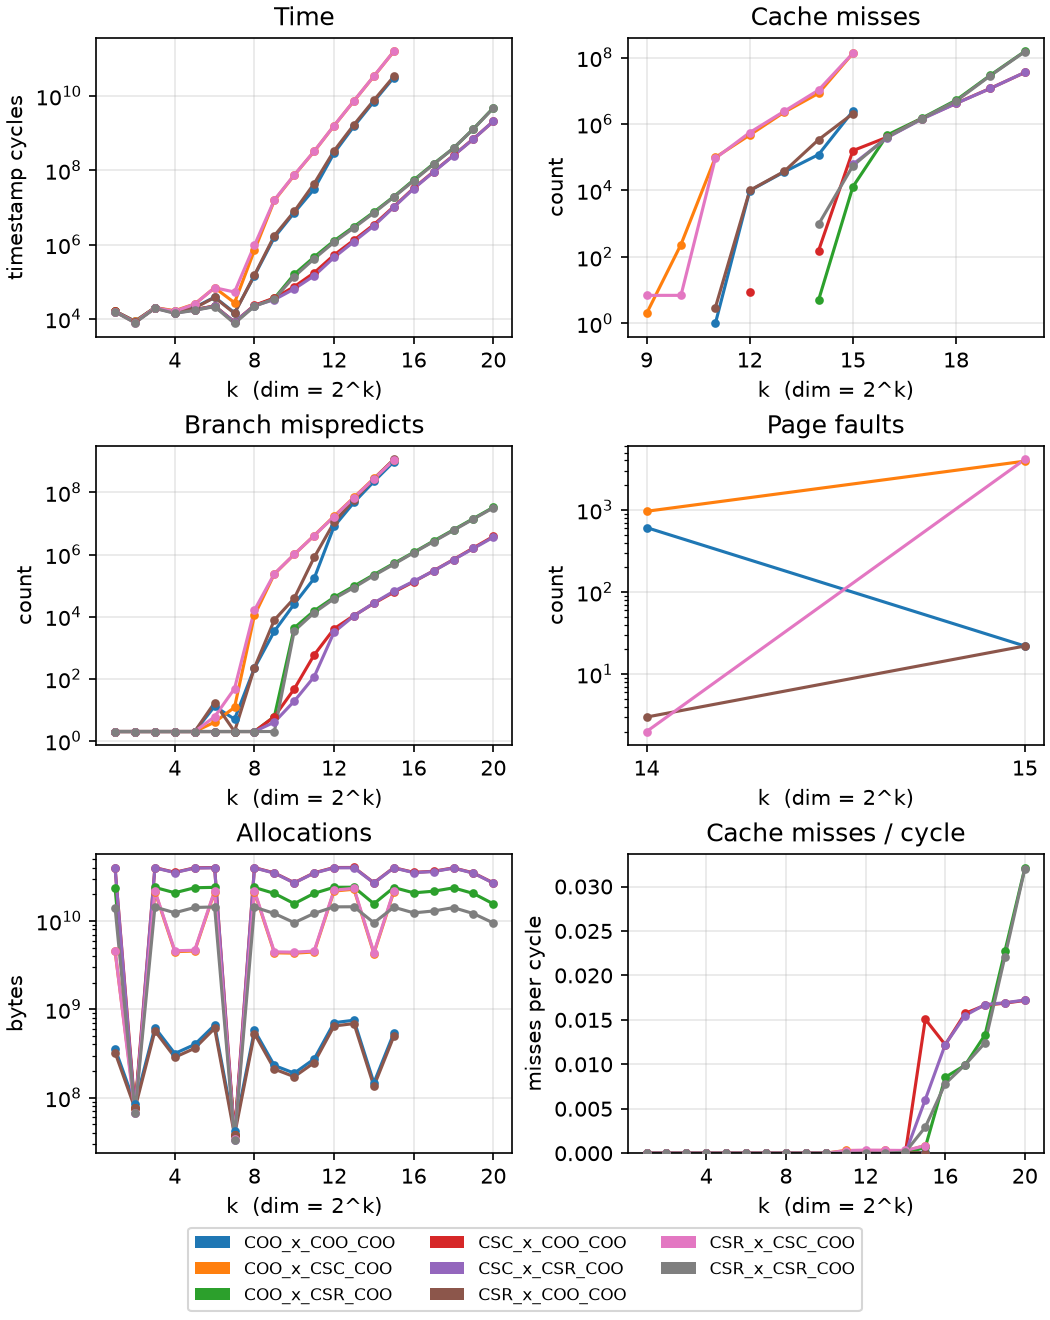
\includegraphics[width=0.85\linewidth,height=0.75\textheight,keepaspectratio]{figures/formats_Cit-Hep-Th_s2.png}
    \caption{Cit-Hep-Th Sample 2 comparison.}
    \label{fig:formats_Cit-Hep-Th}
\end{figure}

\begin{figure}[htbp]
    \centering
    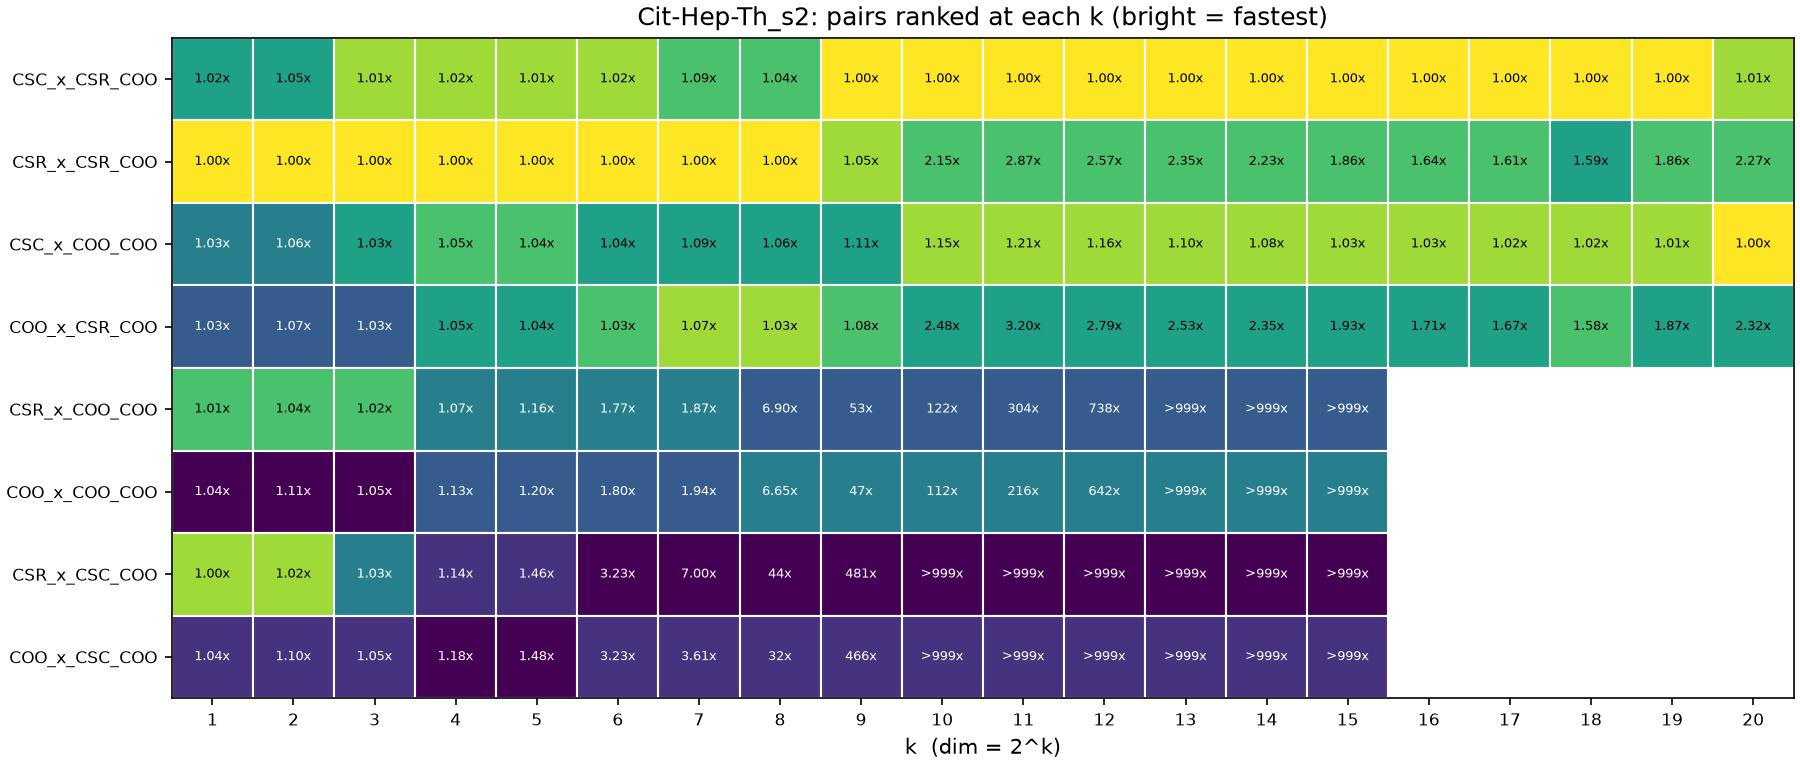
\includegraphics[width=\linewidth,height=0.6\textheight,keepaspectratio]{figures/formats_ranks_Cit-Hep-Th_s2.png}
    \caption{Cit-Hep-Th Sample 2: format pairs ranked at each $k$. Brighter cells are faster; each number is the slowdown relative to the fastest pair at that $k$.}
    \label{fig:formats_ranks_Cit-Hep-Th}
\end{figure}
\clearpage

\begin{figure}[htbp]
    \centering
    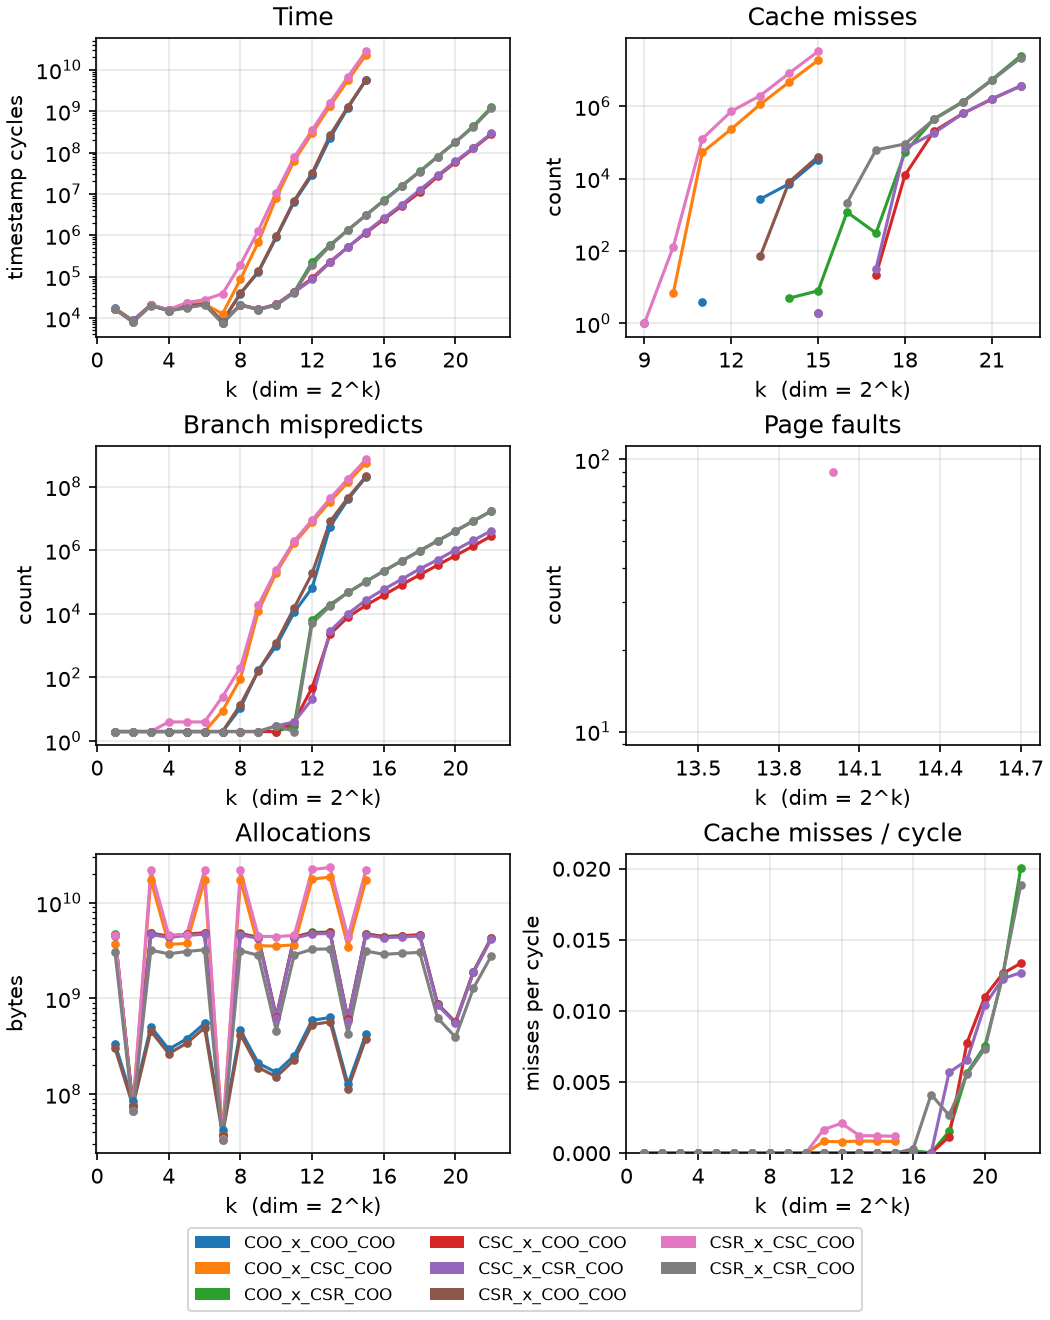
\includegraphics[width=0.85\linewidth,height=0.75\textheight,keepaspectratio]{figures/formats_Delicious_s2.png}
    \caption{Delicious Sample 2 comparison.}
    \label{fig:formats_Delicious}
\end{figure}

\begin{figure}[htbp]
    \centering
    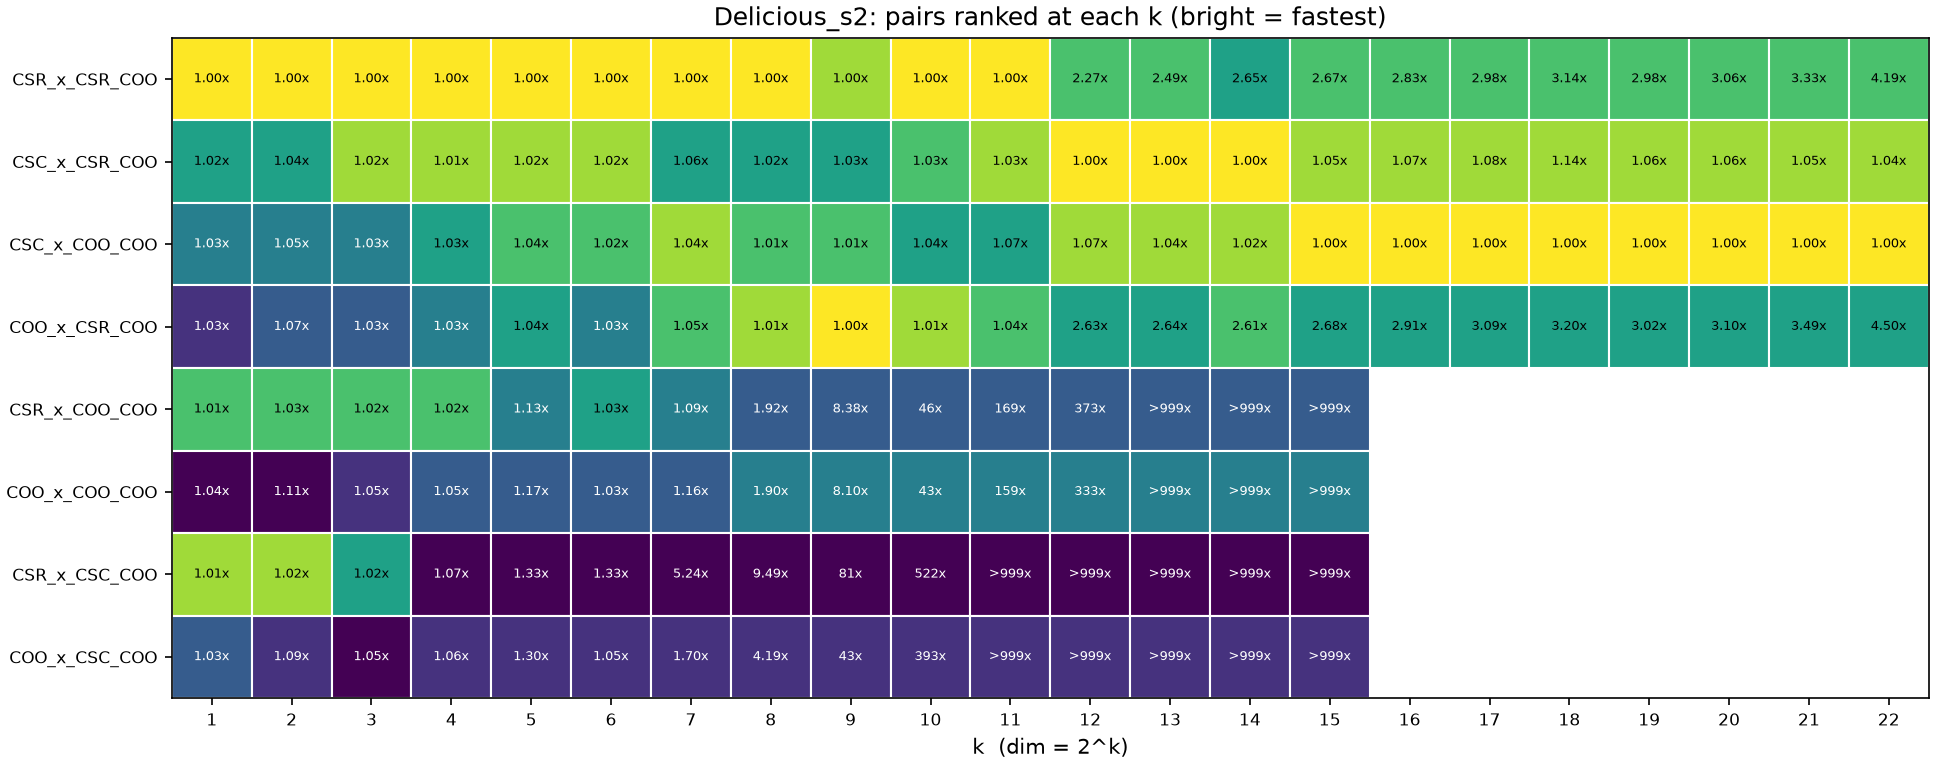
\includegraphics[width=\linewidth,height=0.6\textheight,keepaspectratio]{figures/formats_ranks_Delicious_s2.png}
    \caption{Delicious Sample 2: format pairs ranked at each $k$. Brighter cells are faster; each number is the slowdown relative to the fastest pair at that $k$.}
    \label{fig:formats_ranks_Delicious}
\end{figure}
\clearpage

\begin{figure}[htbp]
    \centering
    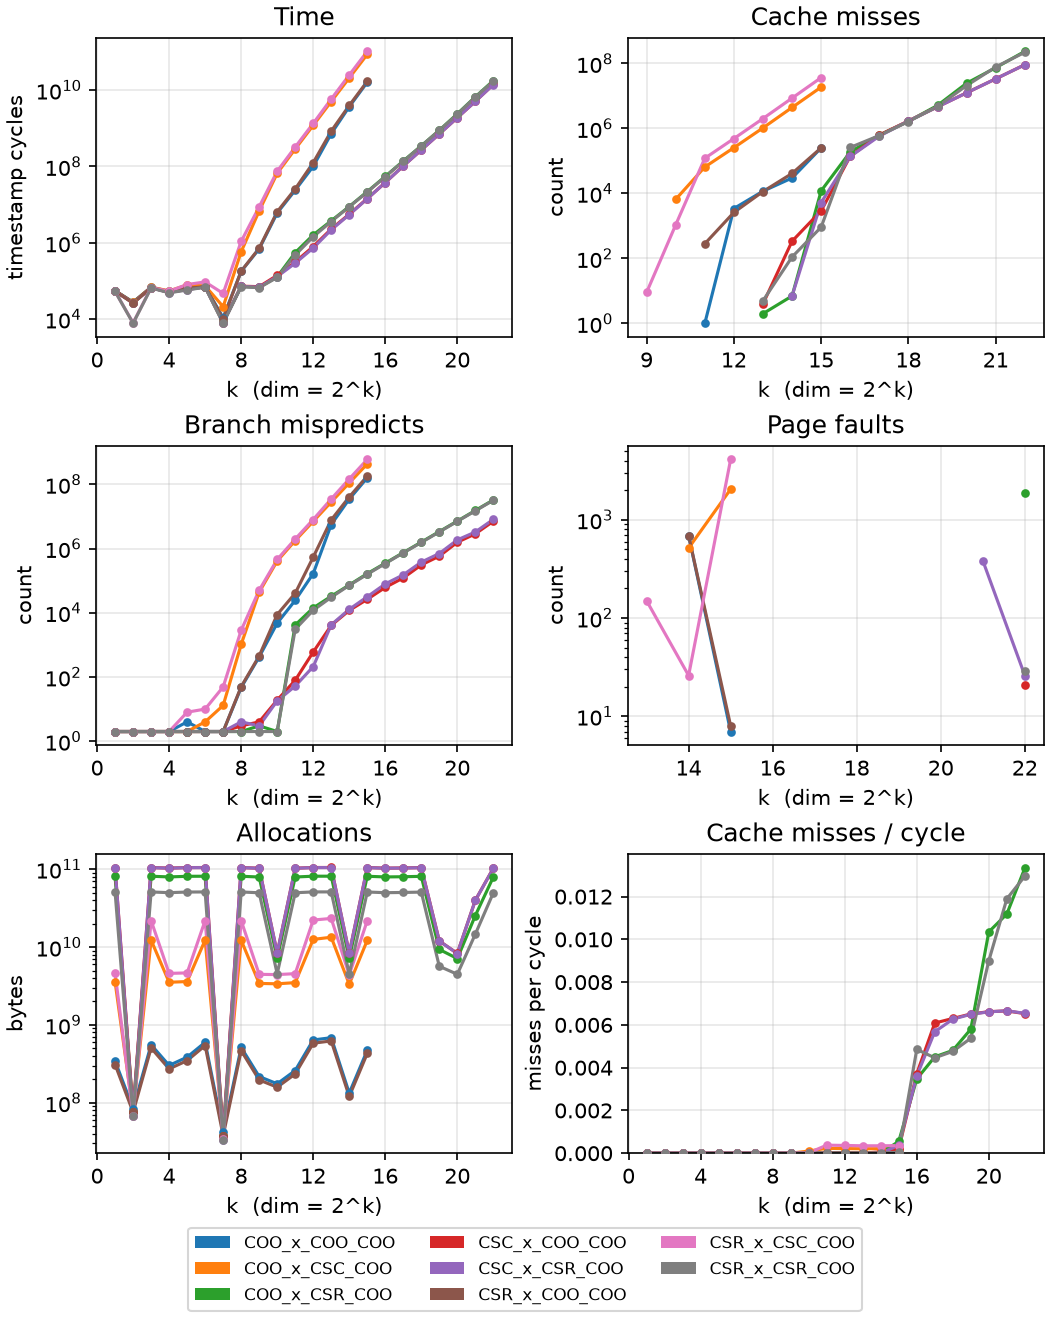
\includegraphics[width=0.85\linewidth,height=0.75\textheight,keepaspectratio]{figures/formats_Epinions_s2.png}
    \caption{Epinions Sample 2 comparison.}
    \label{fig:formats_Epinions}
\end{figure}

\begin{figure}[htbp]
    \centering
    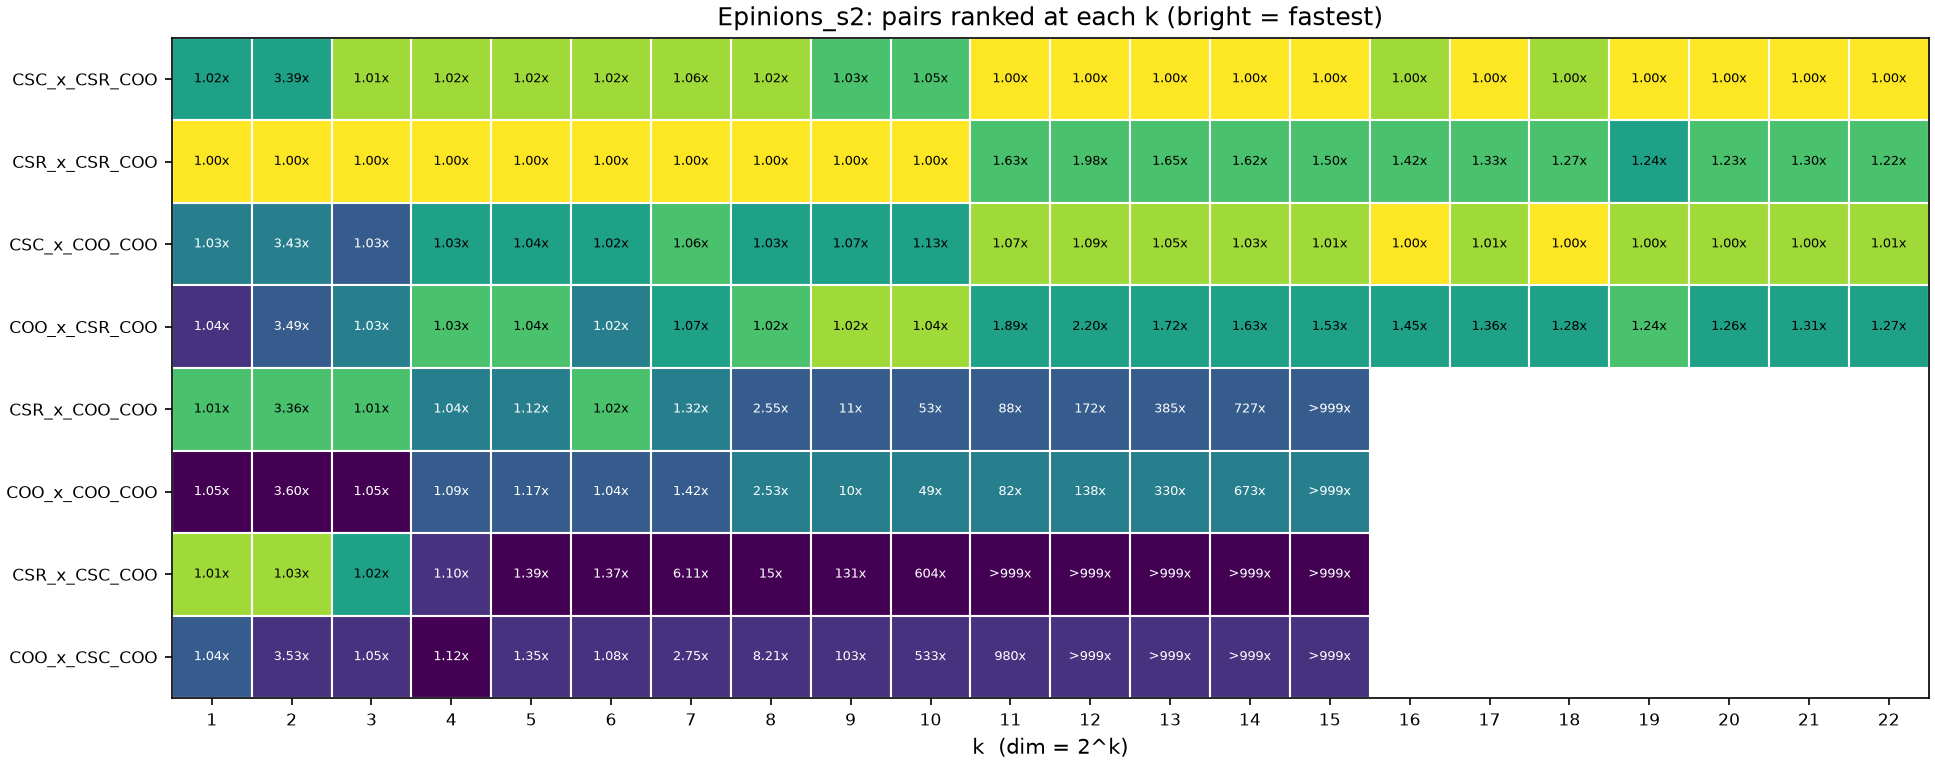
\includegraphics[width=\linewidth,height=0.6\textheight,keepaspectratio]{figures/formats_ranks_Epinions_s2.png}
    \caption{Epinions Sample 2: format pairs ranked at each $k$. Brighter cells are faster; each number is the slowdown relative to the fastest pair at that $k$.}
    \label{fig:formats_ranks_Epinions}
\end{figure}
\clearpage

\begin{figure}[htbp]
    \centering
    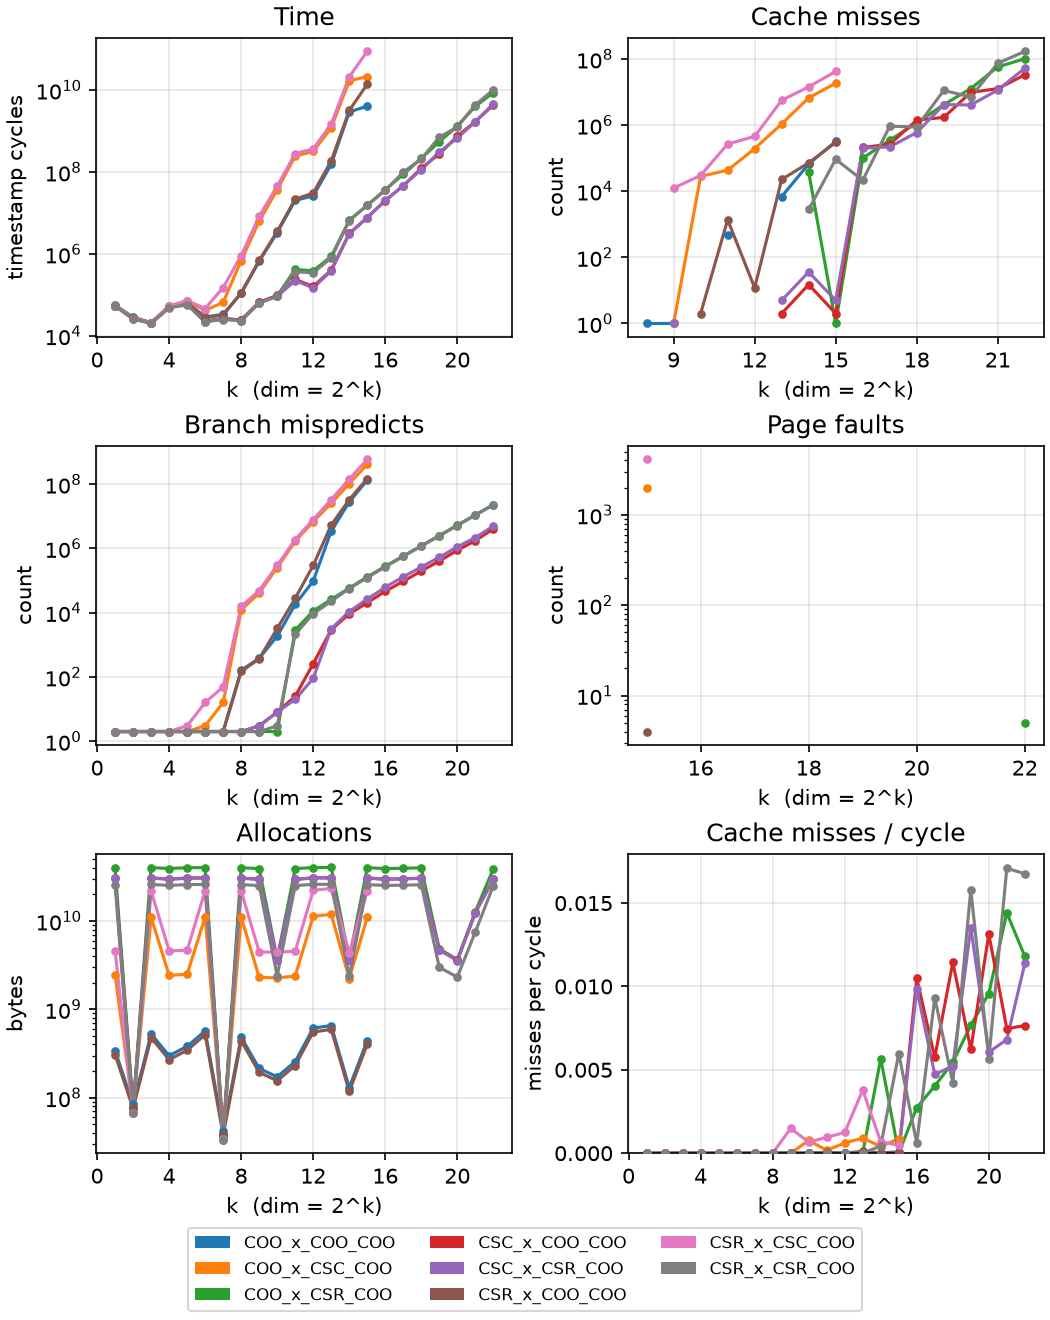
\includegraphics[width=0.85\linewidth,height=0.75\textheight,keepaspectratio]{figures/formats_Flickr_s2.png}
    \caption{Flickr Sample 2 comparison.}
    \label{fig:formats_Flickr}
\end{figure}

\begin{figure}[htbp]
    \centering
    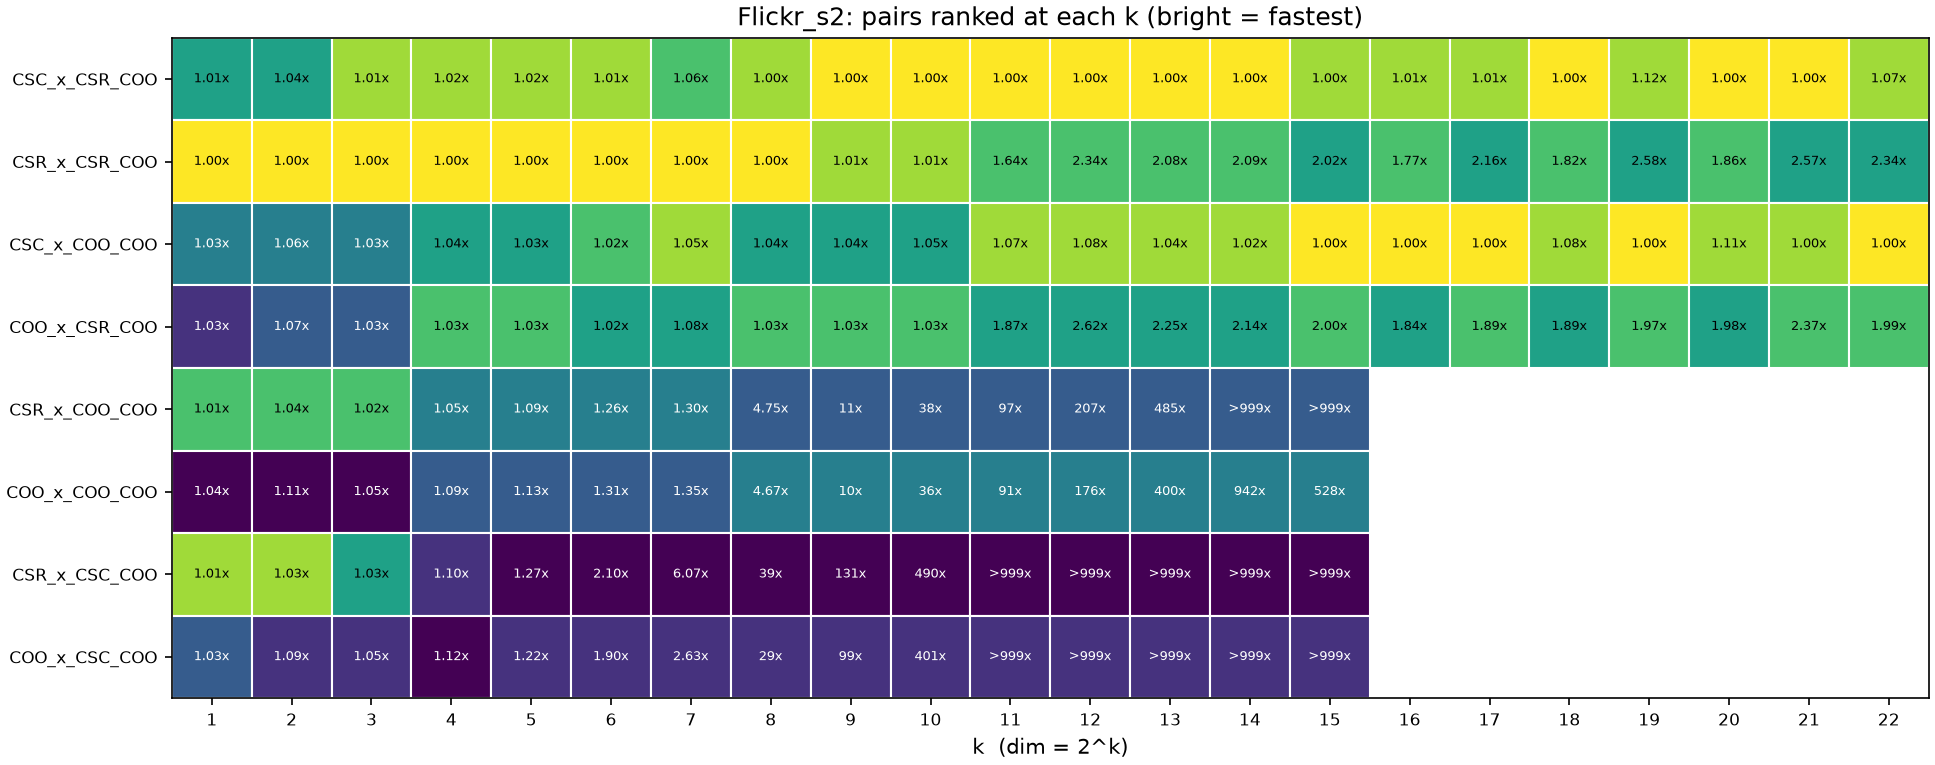
\includegraphics[width=\linewidth,height=0.6\textheight,keepaspectratio]{figures/formats_ranks_Flickr_s2.png}
    \caption{Flickr Sample 2: format pairs ranked at each $k$. Brighter cells are faster; each number is the slowdown relative to the fastest pair at that $k$.}
    \label{fig:formats_ranks_Flickr}
\end{figure}
\clearpage

\begin{figure}[htbp]
    \centering
    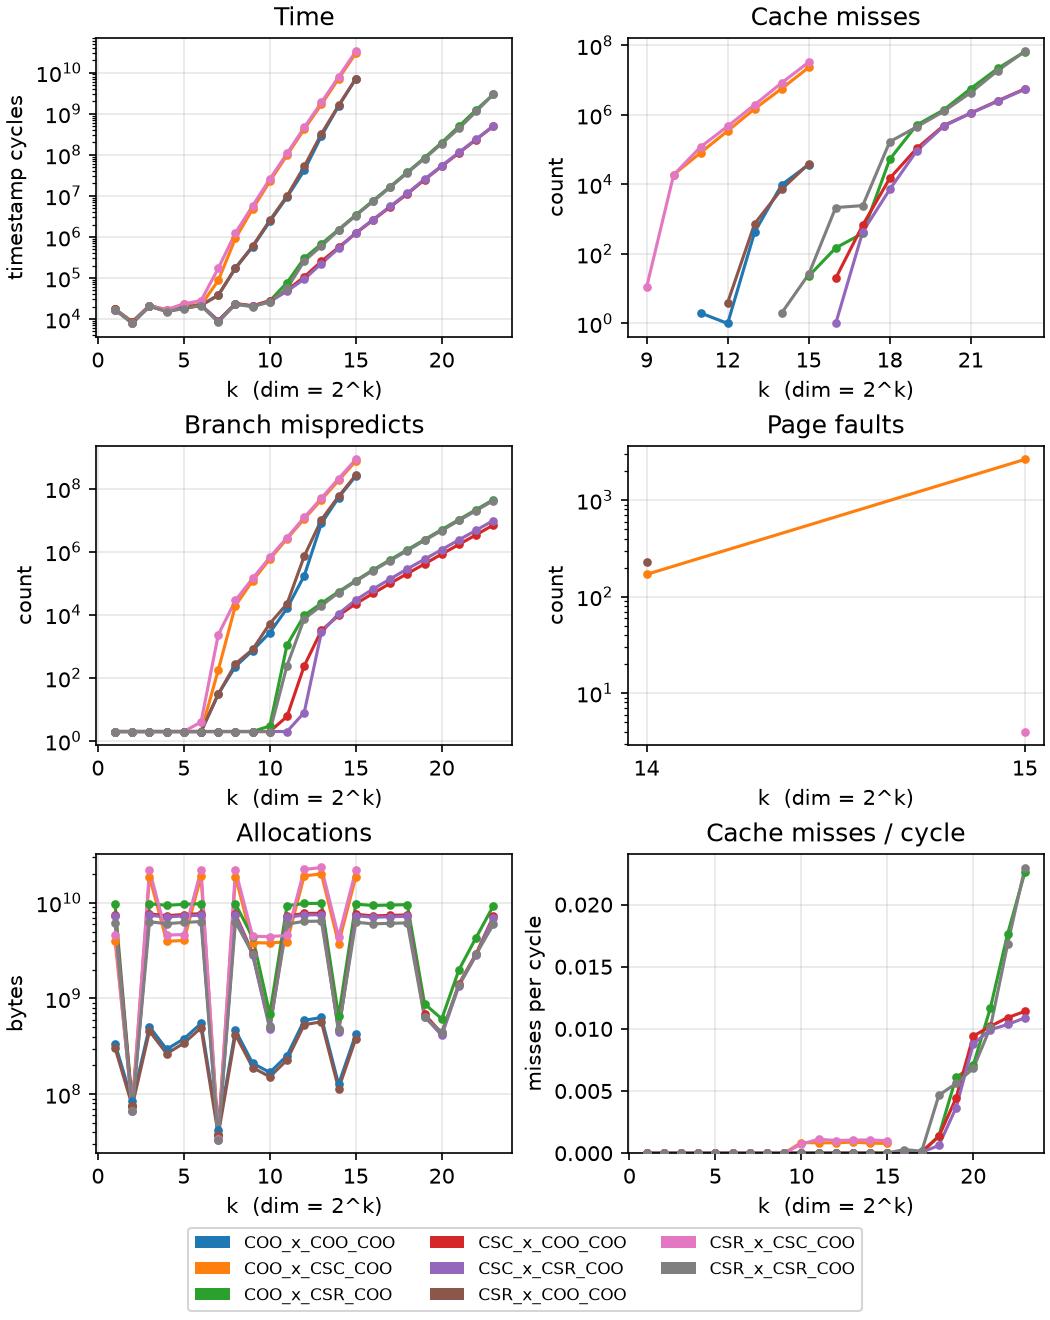
\includegraphics[width=0.85\linewidth,height=0.75\textheight,keepaspectratio]{figures/formats_Gnutella-25_s2.png}
    \caption{Gnutella-25 Sample 2 comparison.}
    \label{fig:formats_Gnutella-25}
\end{figure}

\begin{figure}[htbp]
    \centering
    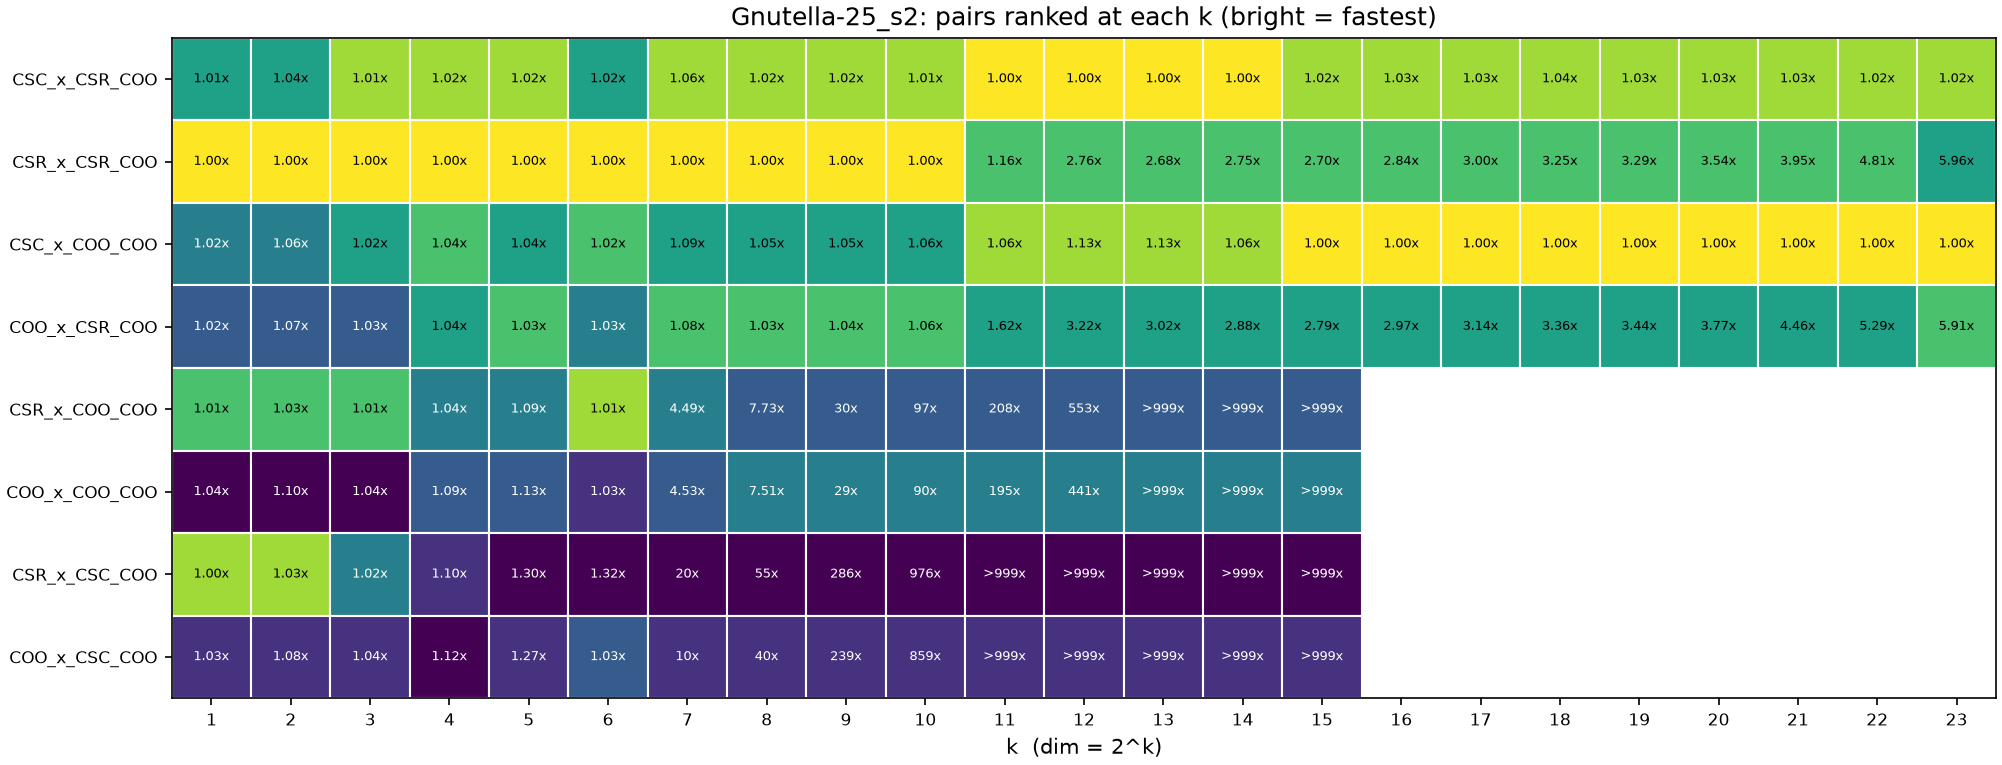
\includegraphics[width=\linewidth,height=0.6\textheight,keepaspectratio]{figures/formats_ranks_Gnutella-25_s2.png}
    \caption{Gnutella-25 Sample 2: format pairs ranked at each $k$. Brighter cells are faster; each number is the slowdown relative to the fastest pair at that $k$.}
    \label{fig:formats_ranks_Gnutella-25}
\end{figure}
\clearpage

\begin{figure}[htbp]
    \centering
    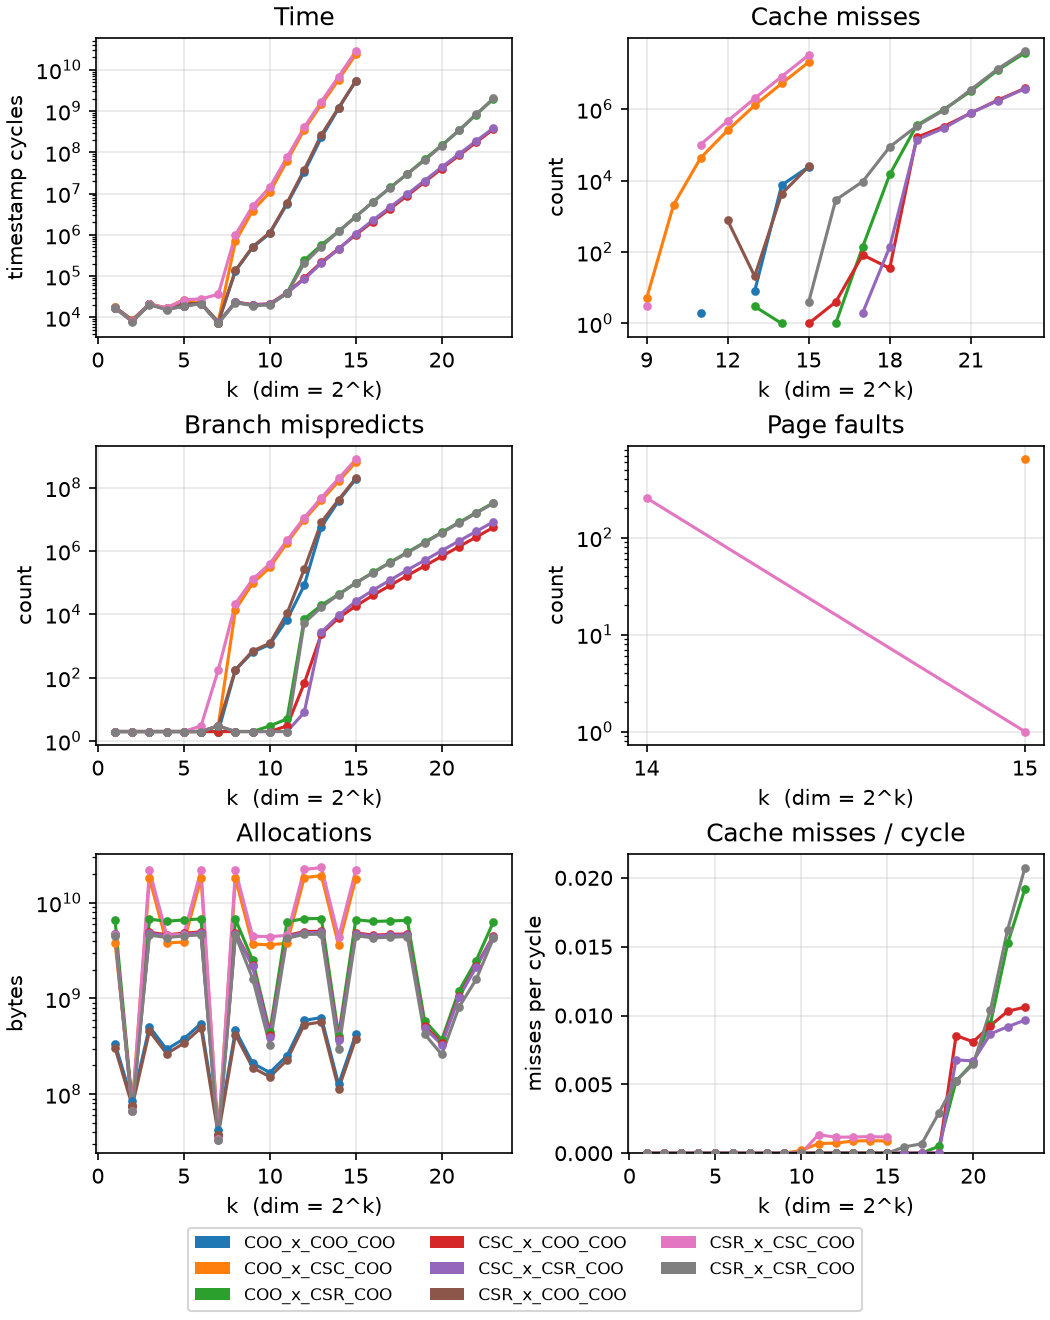
\includegraphics[width=0.85\linewidth,height=0.75\textheight,keepaspectratio]{figures/formats_Gnutella-30_s2.png}
    \caption{Gnutella-30 Sample 2 comparison.}
    \label{fig:formats_Gnutella-30}
\end{figure}

\begin{figure}[htbp]
    \centering
    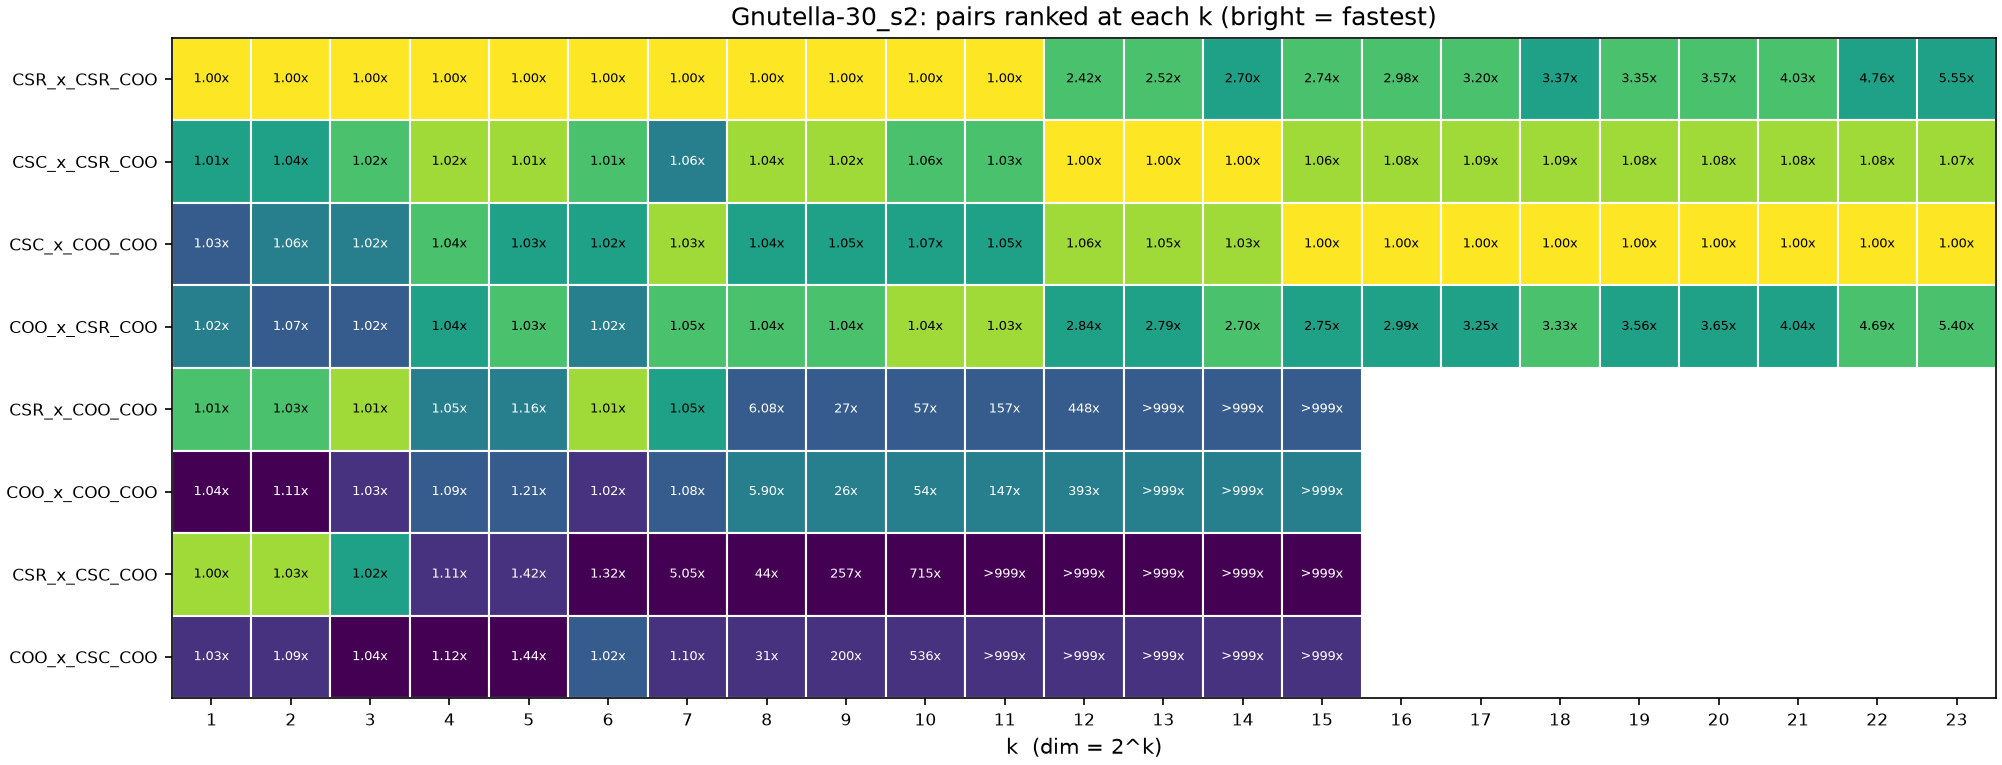
\includegraphics[width=\linewidth,height=0.6\textheight,keepaspectratio]{figures/formats_ranks_Gnutella-30_s2.png}
    \caption{Gnutella-30 Sample 2: format pairs ranked at each $k$. Brighter cells are faster; each number is the slowdown relative to the fastest pair at that $k$.}
    \label{fig:formats_ranks_Gnutella-30}
\end{figure}
\clearpage

\begin{figure}[htbp]
    \centering
    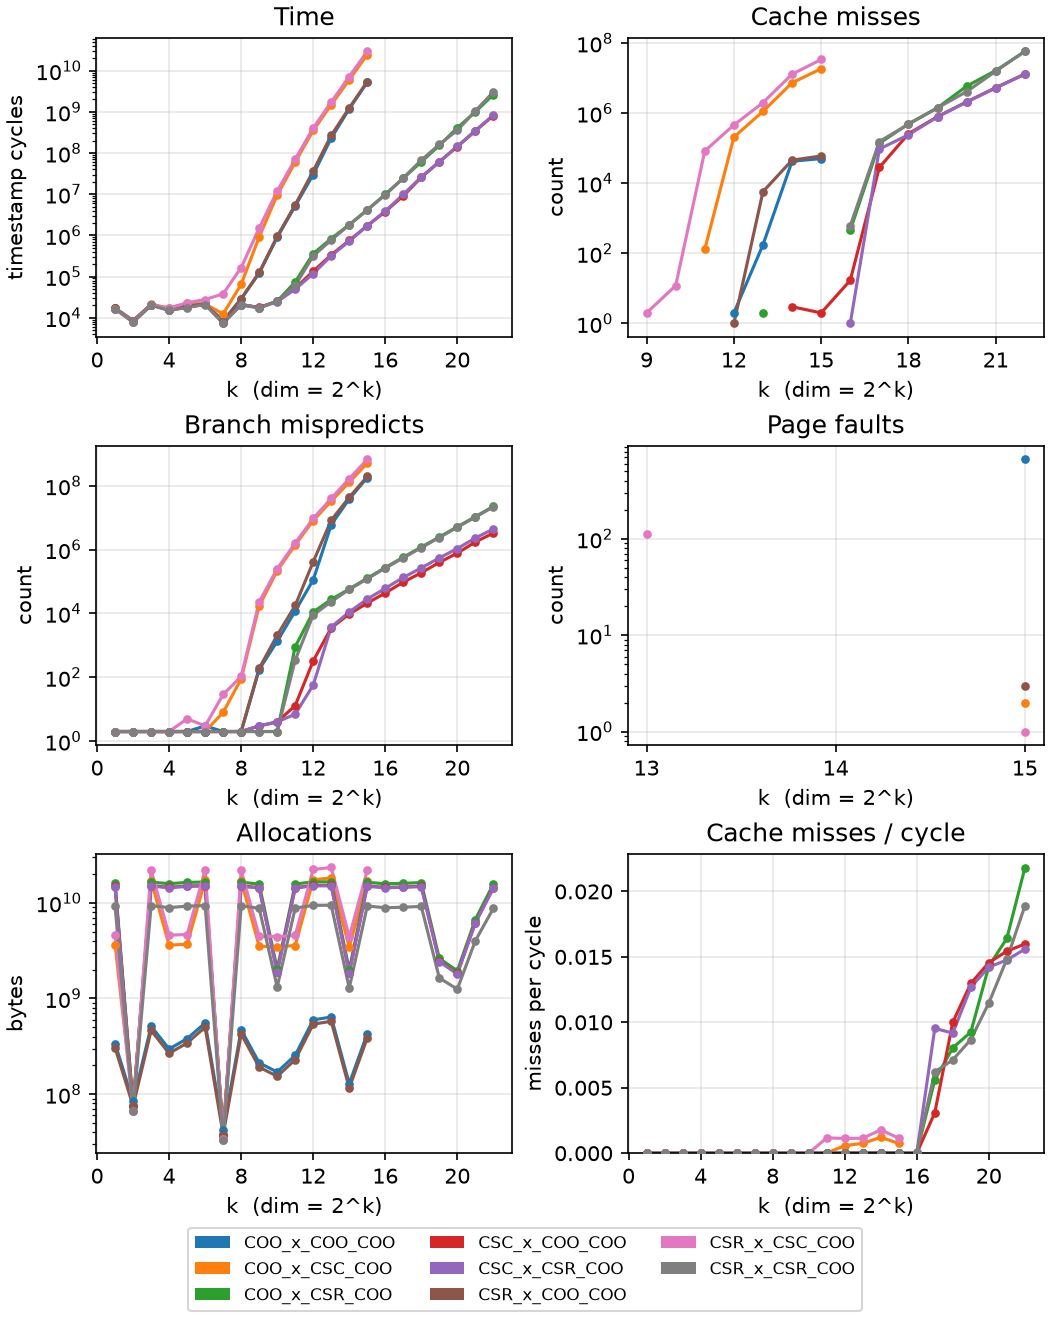
\includegraphics[width=0.85\linewidth,height=0.75\textheight,keepaspectratio]{figures/formats_Web-Notredame_s2.png}
    \caption{Web-Notredame Sample 2 comparison.}
    \label{fig:formats_Web-Notredame}
\end{figure}

\begin{figure}[htbp]
    \centering
    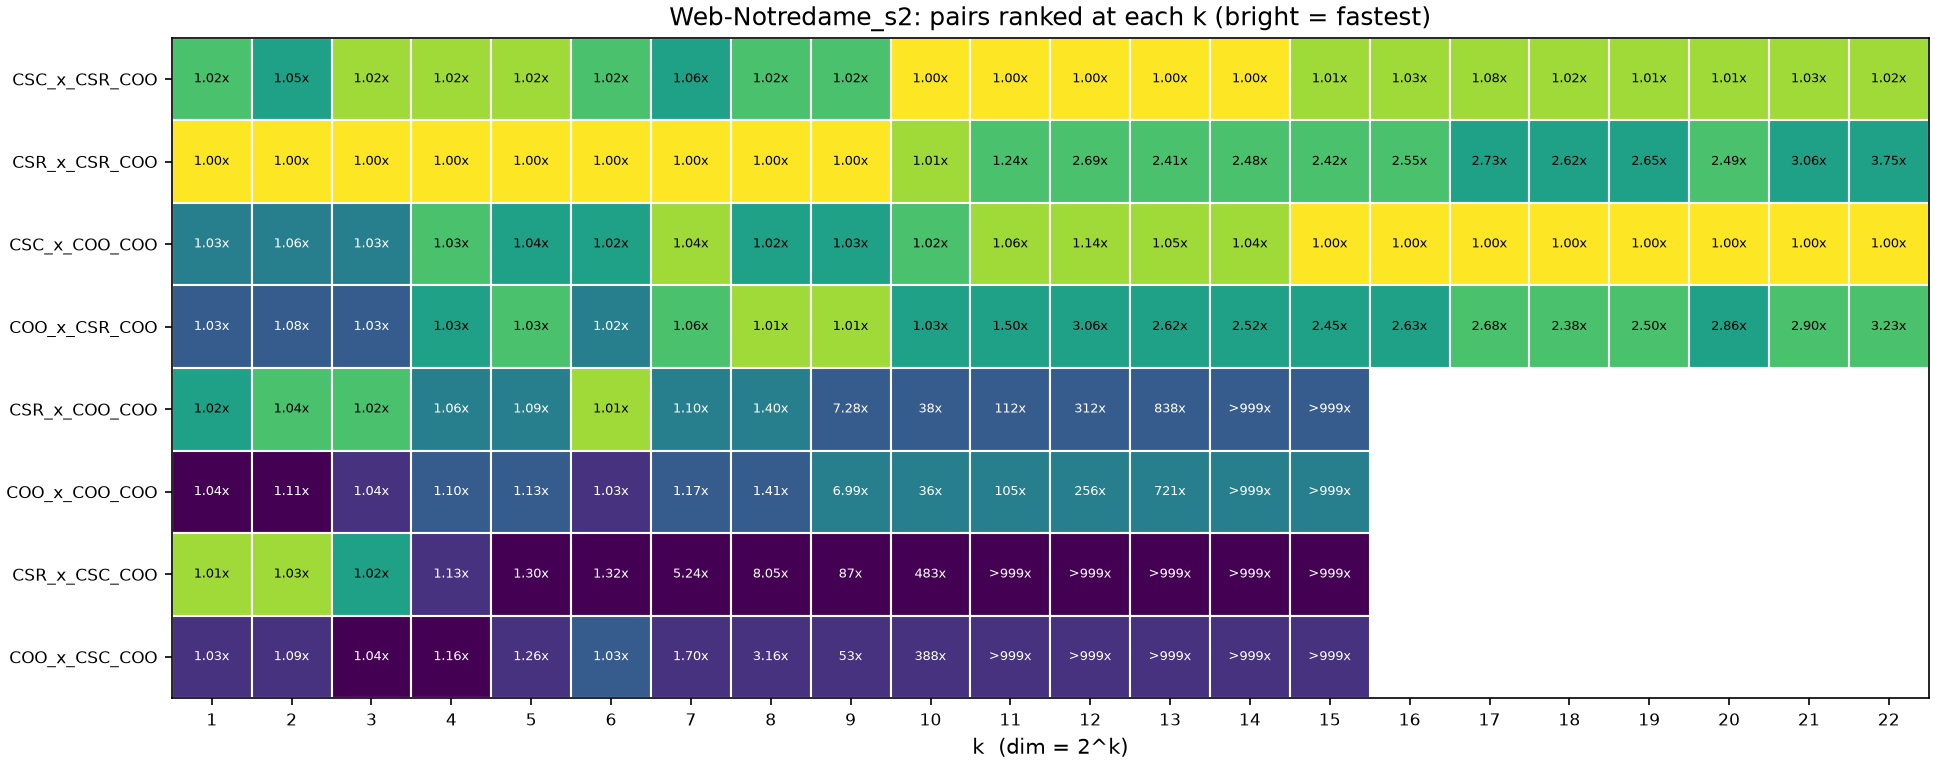
\includegraphics[width=\linewidth,height=0.6\textheight,keepaspectratio]{figures/formats_ranks_Web-Notredame_s2.png}
    \caption{Web-Notredame Sample 2: format pairs ranked at each $k$. Brighter cells are faster; each number is the slowdown relative to the fastest pair at that $k$.}
    \label{fig:formats_ranks_Web-Notredame}
\end{figure}
\clearpage

\chapter{Tiling Figures}
\label{app:tiling_figs}

\begin{figure}[htbp]
  \centering
  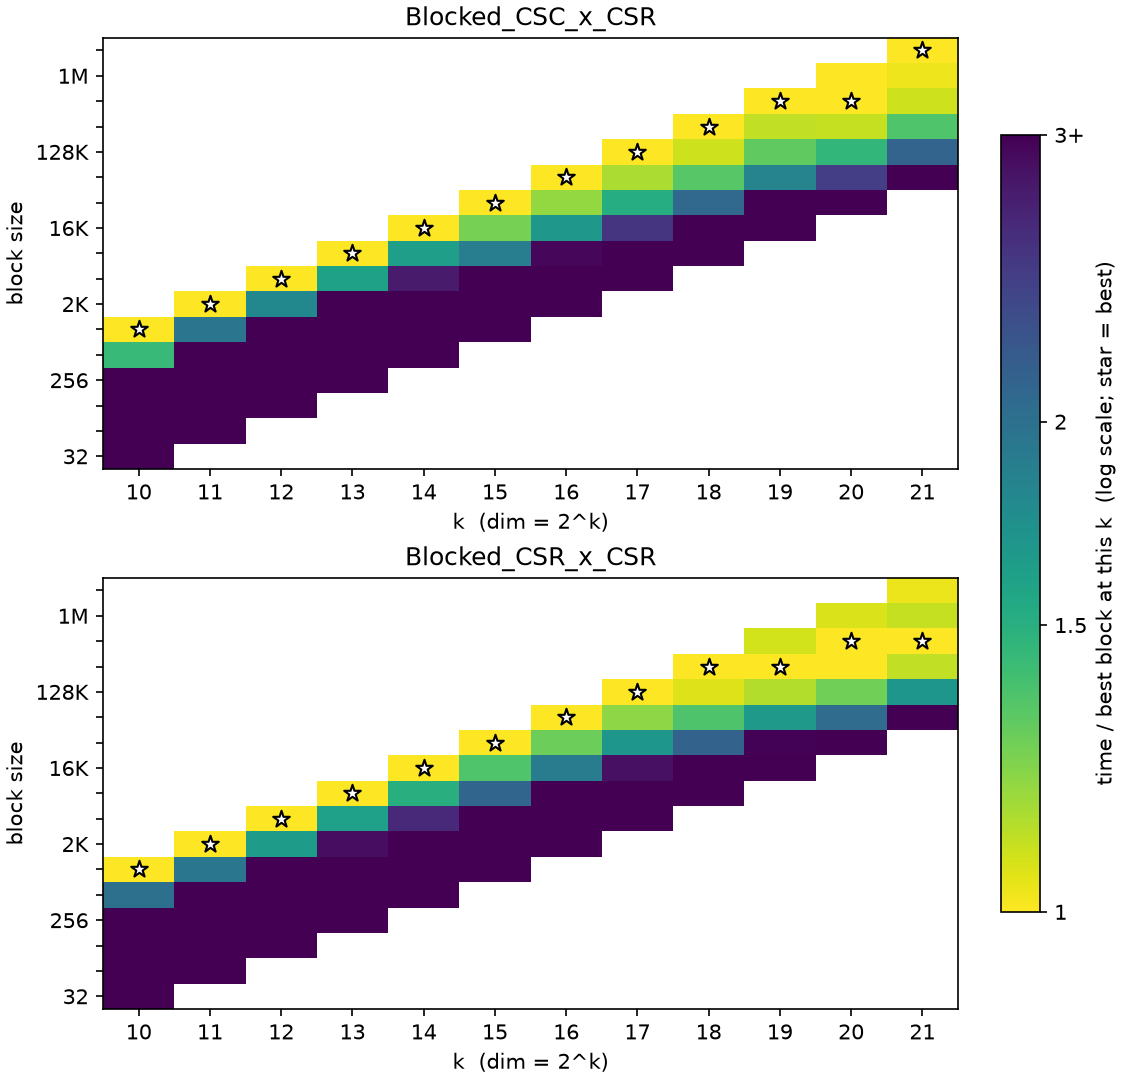
\includegraphics[width=0.9\linewidth,height=0.75\textheight,keepaspectratio]{figures/tiled_AS-Newman_s2.png}
  \caption{AS-Newman Sample 2 tiled block-size sweep. Colour is time relative to the best block size at each $k$ (1 is best); stars mark the best block size.}
  \label{fig:tiled_AS-Newman}
\end{figure}
\clearpage

\begin{figure}[htbp]
  \centering
  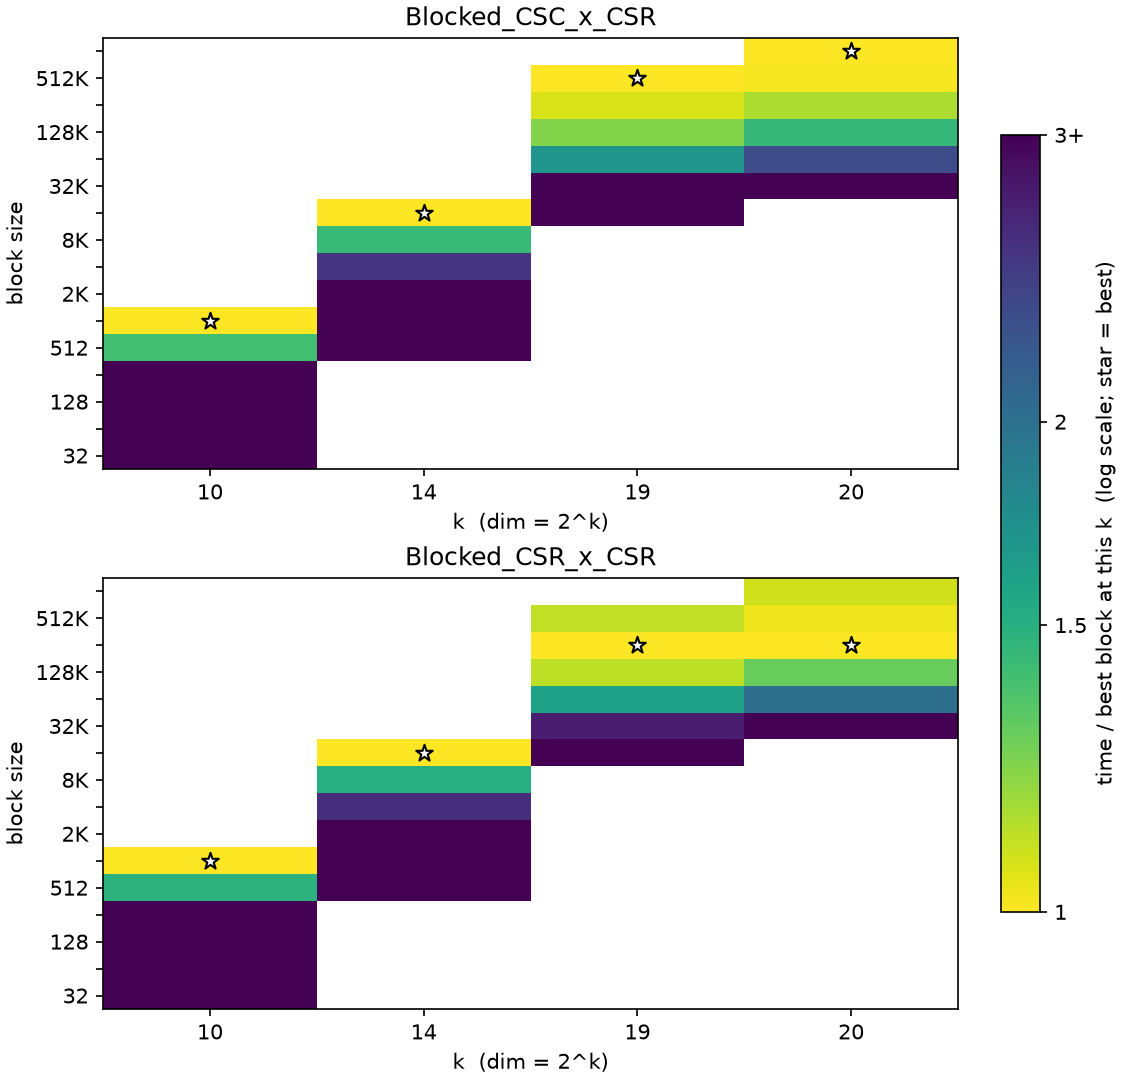
\includegraphics[width=0.9\linewidth,height=0.75\textheight,keepaspectratio]{figures/tiled_AS-RouteViews_s2.png}
  \caption{AS-RouteViews Sample 2 tiled block-size sweep. Colour is time relative to the best block size at each $k$ (1 is best); stars mark the best block size.}
  \label{fig:tiled_AS-RouteViews}
\end{figure}
\clearpage

\begin{figure}[htbp]
  \centering
  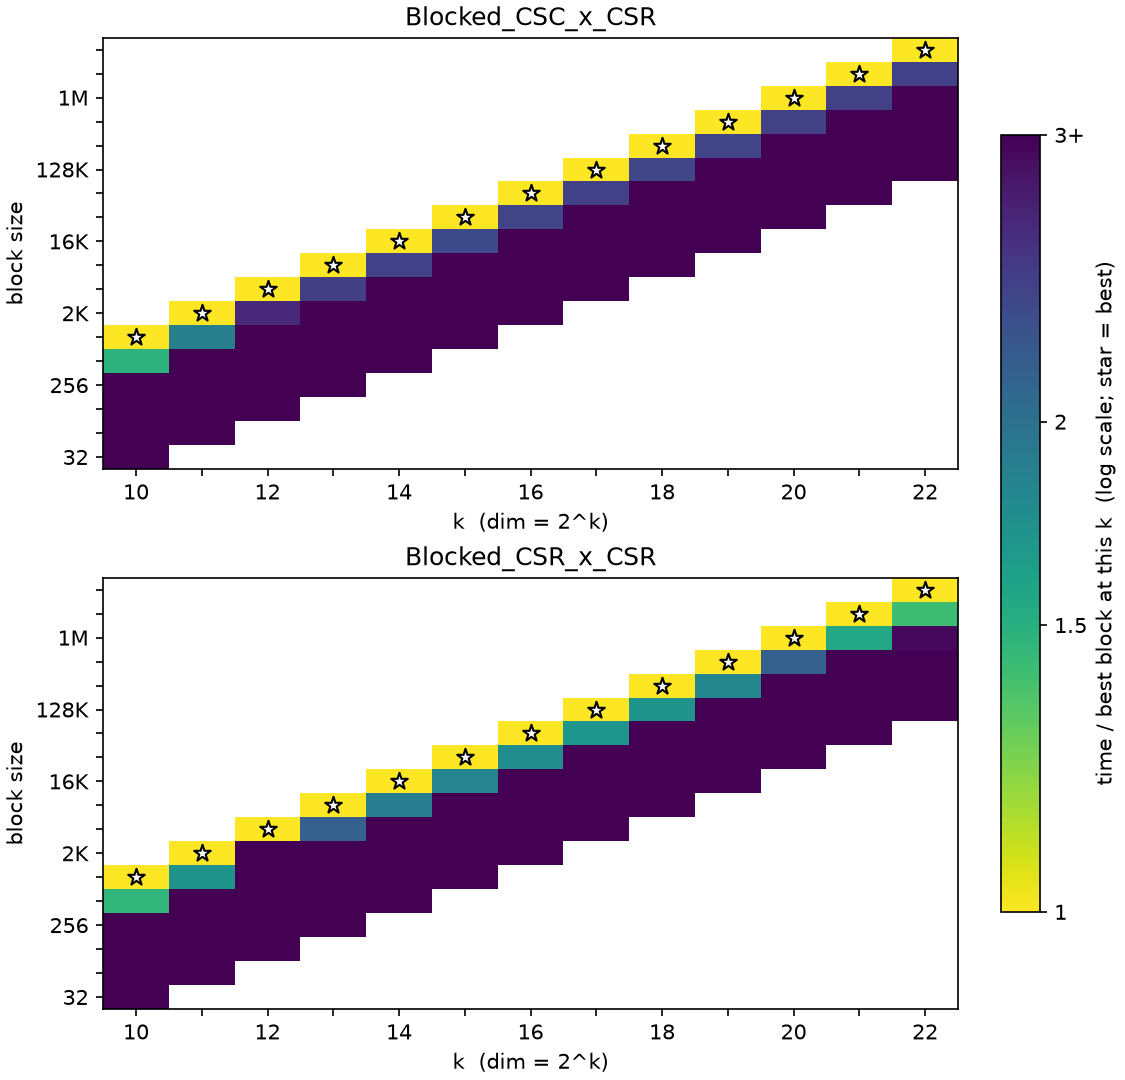
\includegraphics[width=0.9\linewidth,height=0.75\textheight,keepaspectratio]{figures/tiled_ATP-GR-QC_s2.png}
  \caption{ATP-GR-QC Sample 2 tiled block-size sweep. Colour is time relative to the best block size at each $k$ (1 is best); stars mark the best block size.}
  \label{fig:tiled_ATP-GR-QC}
\end{figure}
\clearpage

\begin{figure}[htbp]
  \centering
  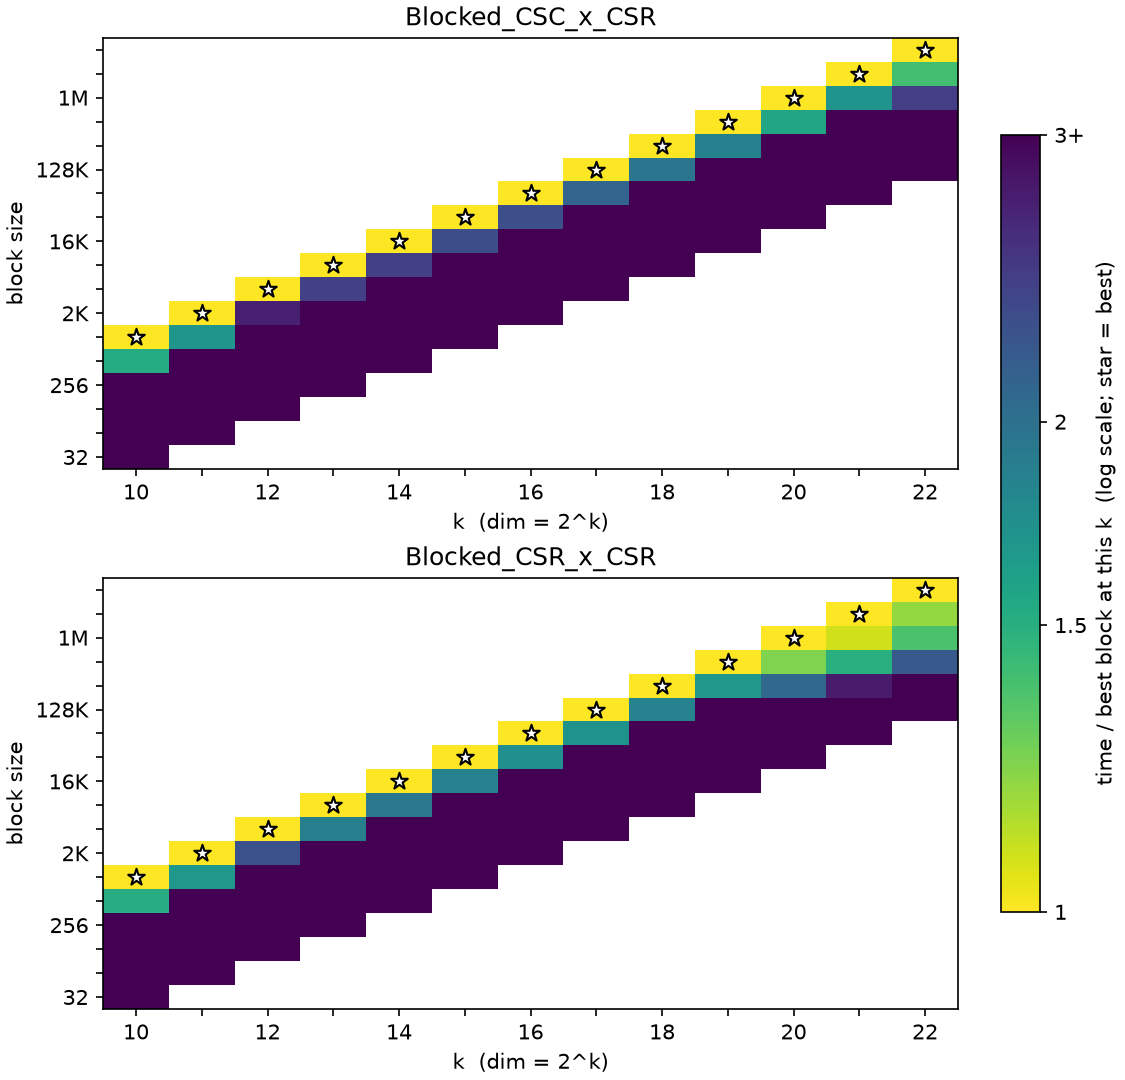
\includegraphics[width=0.9\linewidth,height=0.75\textheight,keepaspectratio]{figures/tiled_Answers_s2.png}
  \caption{Answers Sample 2 tiled block-size sweep. Colour is time relative to the best block size at each $k$ (1 is best); stars mark the best block size.}
  \label{fig:tiled_Answers}
\end{figure}
\clearpage

\begin{figure}[htbp]
  \centering
  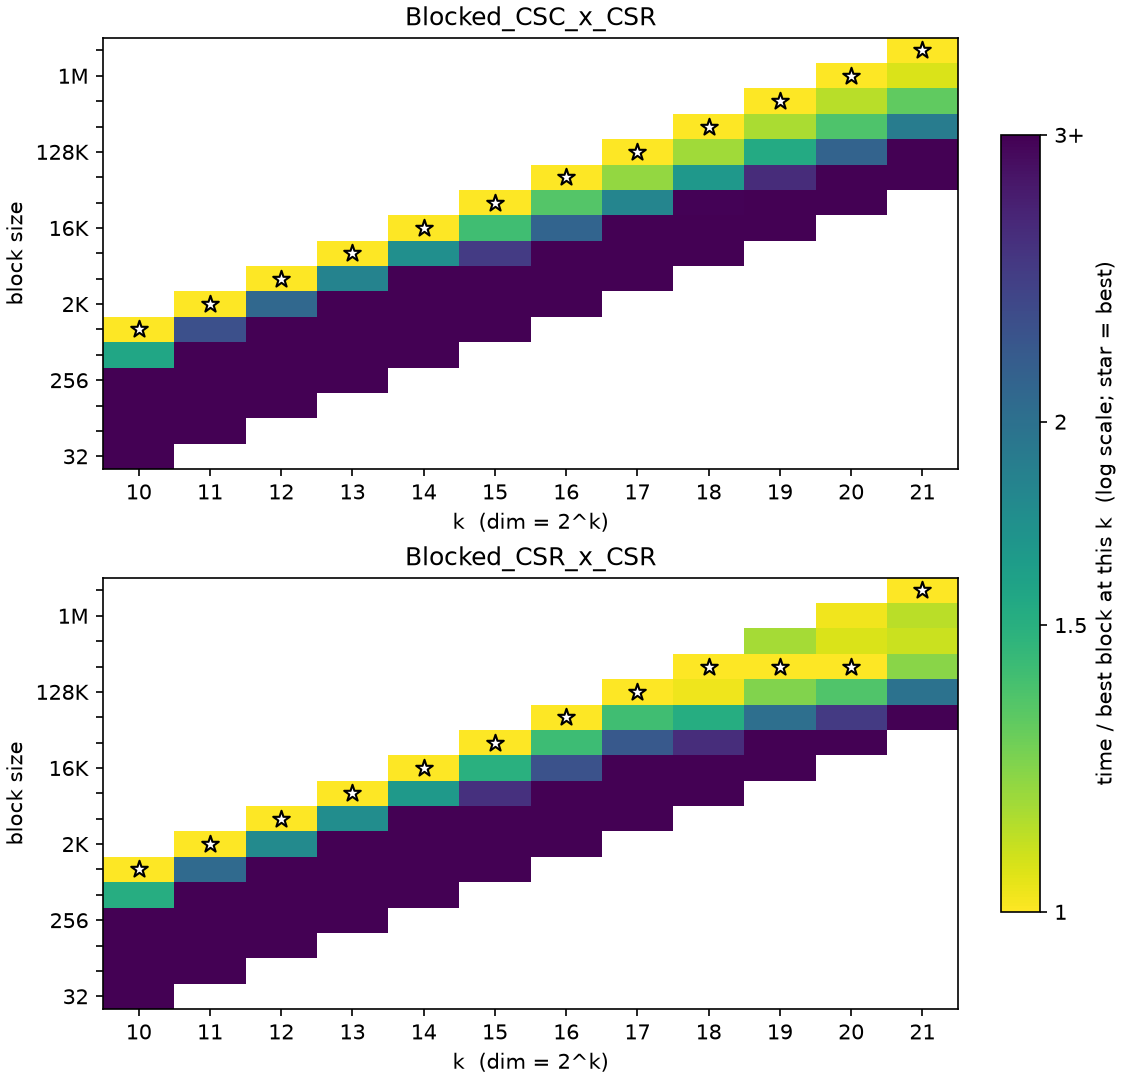
\includegraphics[width=0.9\linewidth,height=0.75\textheight,keepaspectratio]{figures/tiled_Bio-Proteins_s2.png}
  \caption{Bio-Proteins Sample 2 tiled block-size sweep. Colour is time relative to the best block size at each $k$ (1 is best); stars mark the best block size.}
  \label{fig:tiled_Bio-Proteins}
\end{figure}
\clearpage

\begin{figure}[htbp]
  \centering
  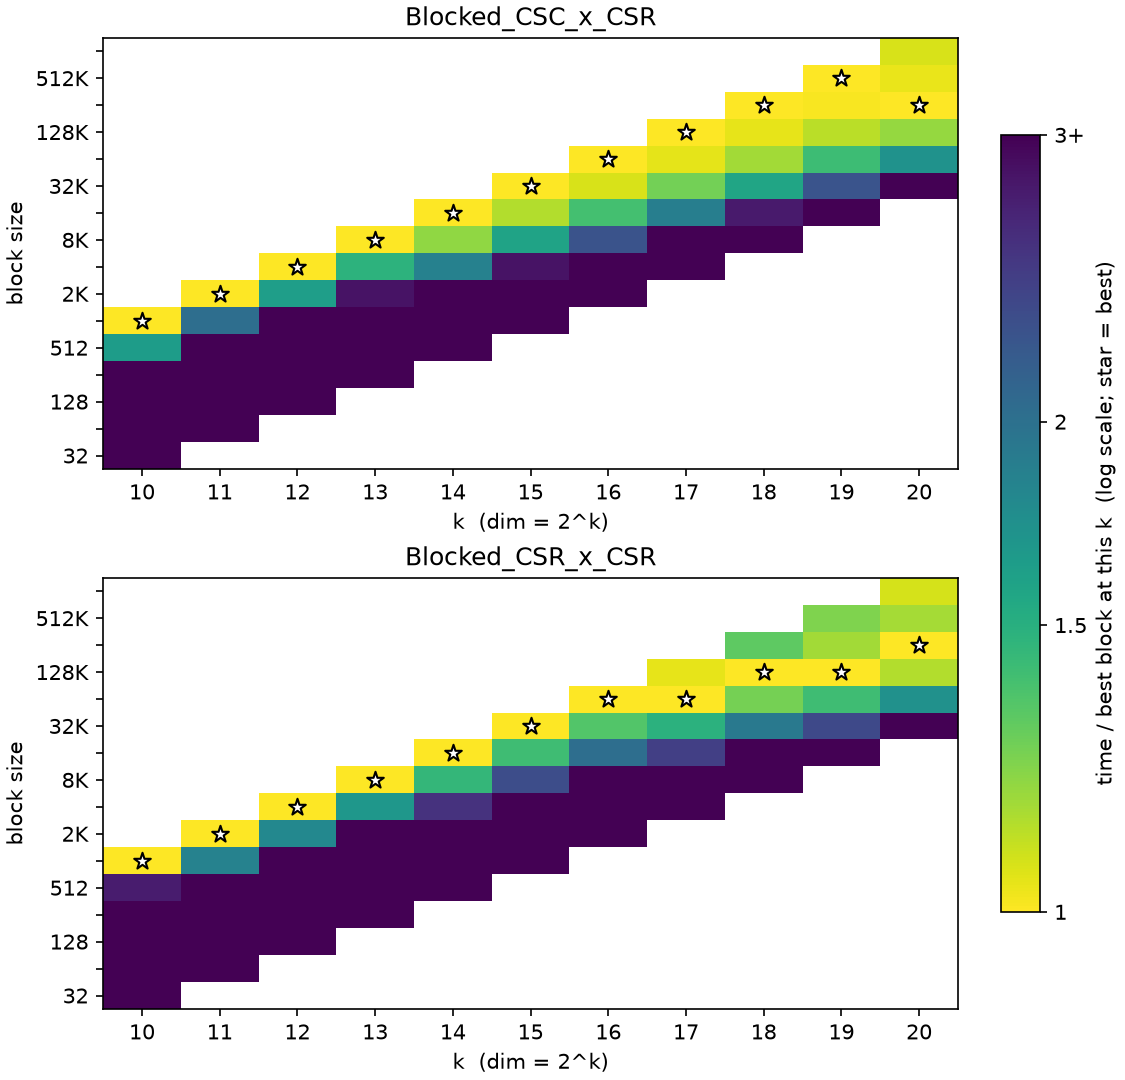
\includegraphics[width=0.9\linewidth,height=0.75\textheight,keepaspectratio]{figures/tiled_Blog-Nat05-6m_s2.png}
  \caption{Blog-Nat05-6m Sample 2 tiled block-size sweep. Colour is time relative to the best block size at each $k$ (1 is best); stars mark the best block size.}
  \label{fig:tiled_Blog-Nat05-6m}
\end{figure}
\clearpage

\begin{figure}[htbp]
  \centering
  
\includegraphics[width=0.9\linewidth,height=0.75\textheight,keepaspectratio]{figures/tiled_Blog-Nat06all_s2.png}
  \caption{Blog-Nat06all Sample 2 tiled block-size sweep. Colour is time relative to the best block size at each $k$ (1 is best); stars mark the best block size.}
  \label{fig:tiled_Blog-Nat06all}
\end{figure}
\clearpage

\begin{figure}[htbp]
  \centering
  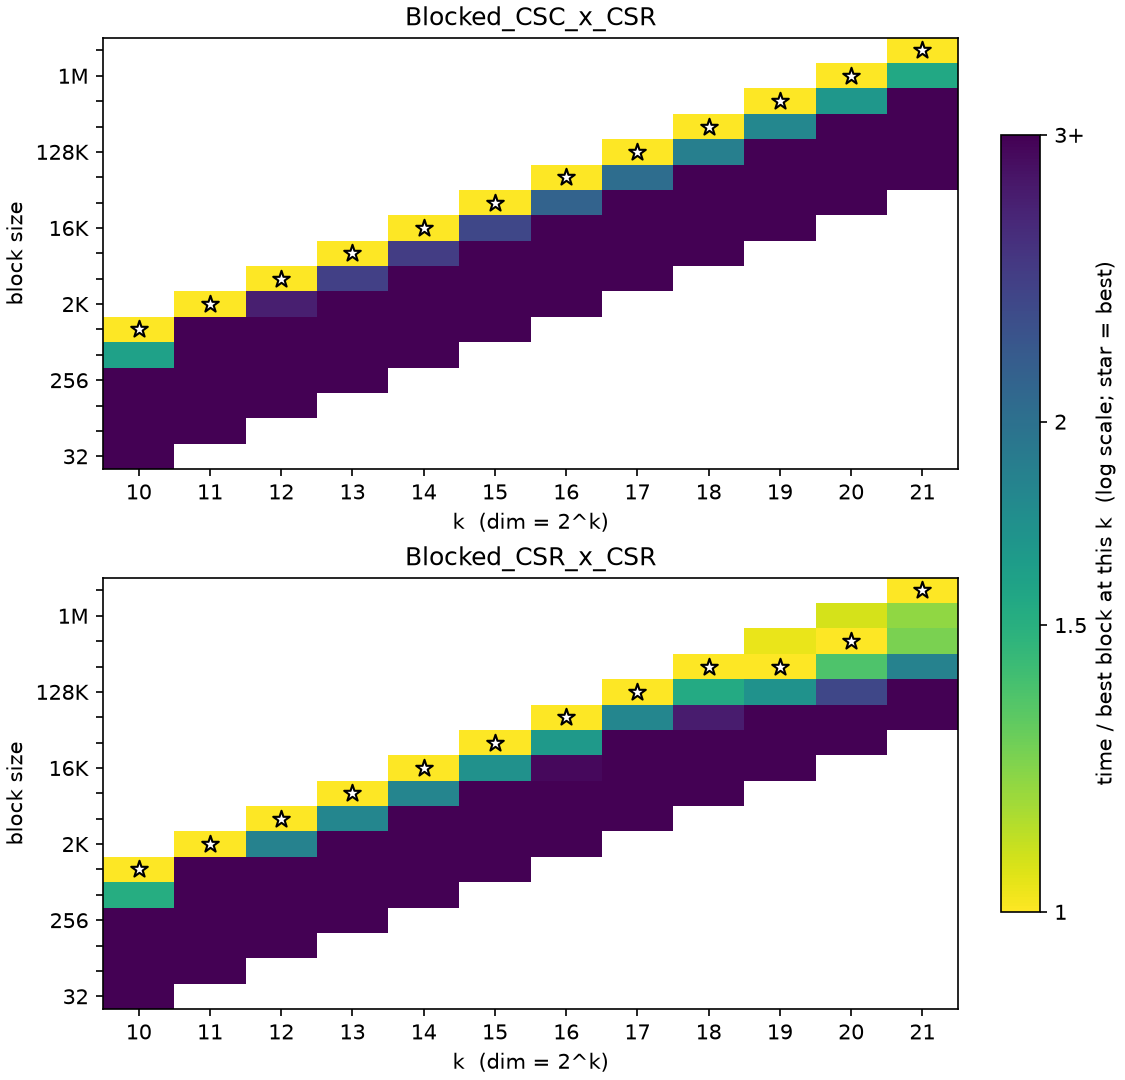
\includegraphics[width=0.9\linewidth,height=0.75\textheight,keepaspectratio]{figures/tiled_CA-DBLP_s2.png}
  \caption{CA-DBLP Sample 2 tiled block-size sweep. Colour is time relative to the best block size at each $k$ (1 is best); stars mark the best block size.}
  \label{fig:tiled_CA-DBLP}
\end{figure}
\clearpage

\begin{figure}[htbp]
  \centering
  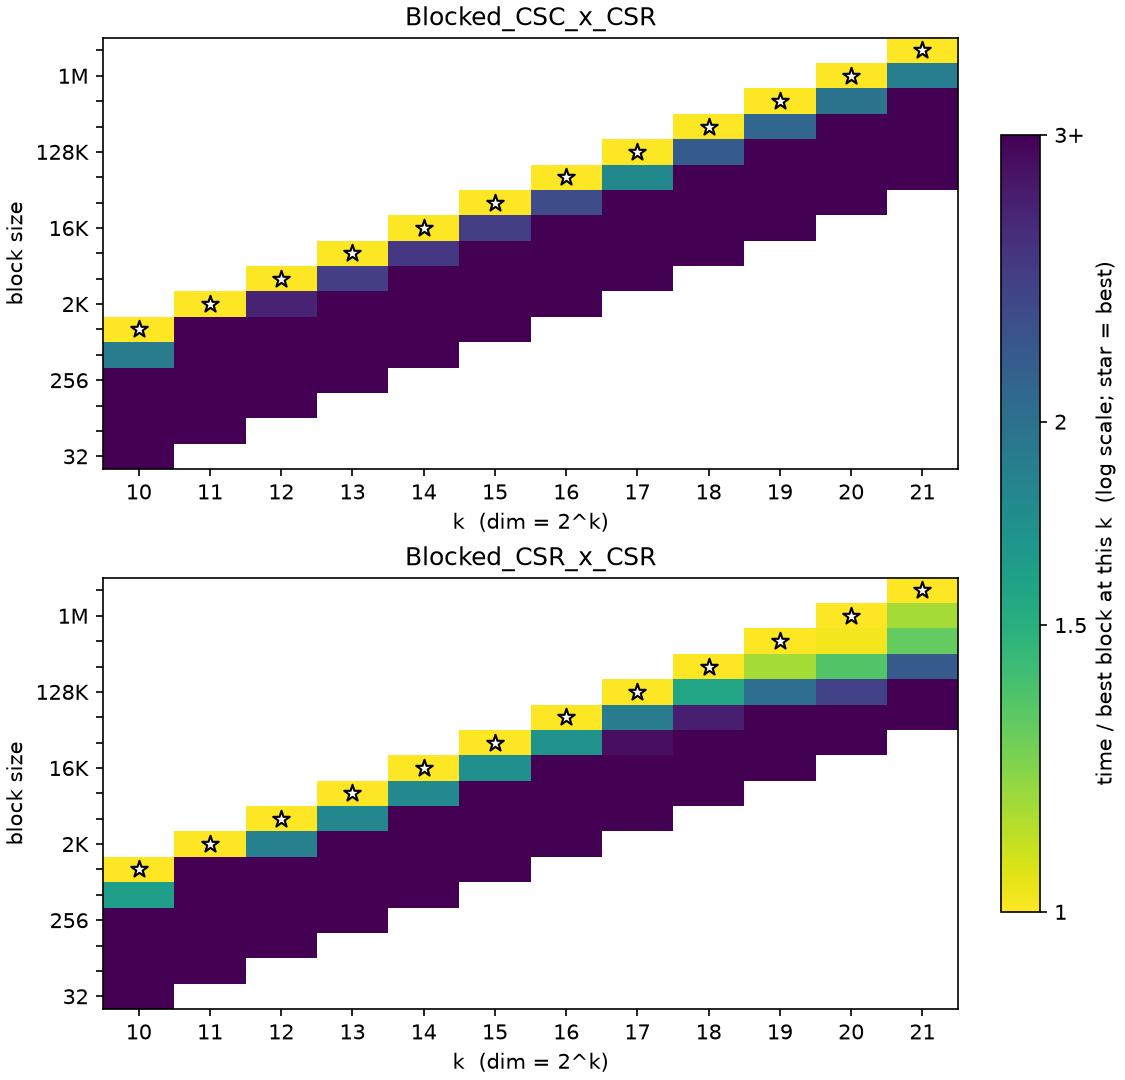
\includegraphics[width=0.9\linewidth,height=0.75\textheight,keepaspectratio]{figures/tiled_CA-GR-QC_s2.png}
  \caption{CA-GR-QC Sample 2 tiled block-size sweep. Colour is time relative to the best block size at each $k$ (1 is best); stars mark the best block size.}
  \label{fig:tiled_CA-GR-QC}
\end{figure}
\clearpage

\begin{figure}[htbp]
  \centering
  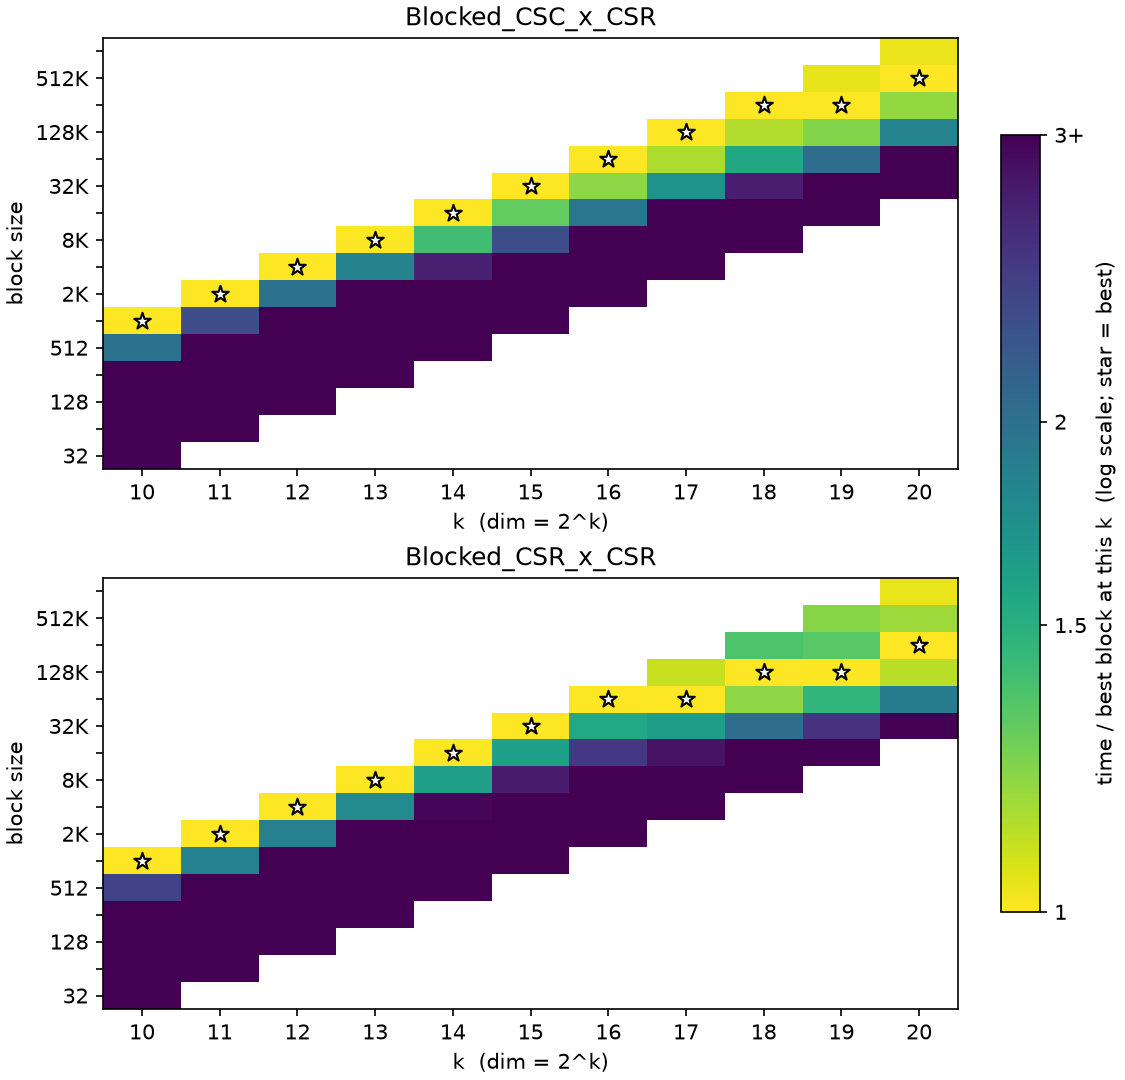
\includegraphics[width=0.9\linewidth,height=0.75\textheight,keepaspectratio]{figures/tiled_CA-Hep-Ph_s2.png}
  \caption{CA-Hep-Ph Sample 2 tiled block-size sweep. Colour is time relative to the best block size at each $k$ (1 is best); stars mark the best block size.}
  \label{fig:tiled_CA-Hep-Ph}
\end{figure}
\clearpage

\begin{figure}[htbp]
  \centering
  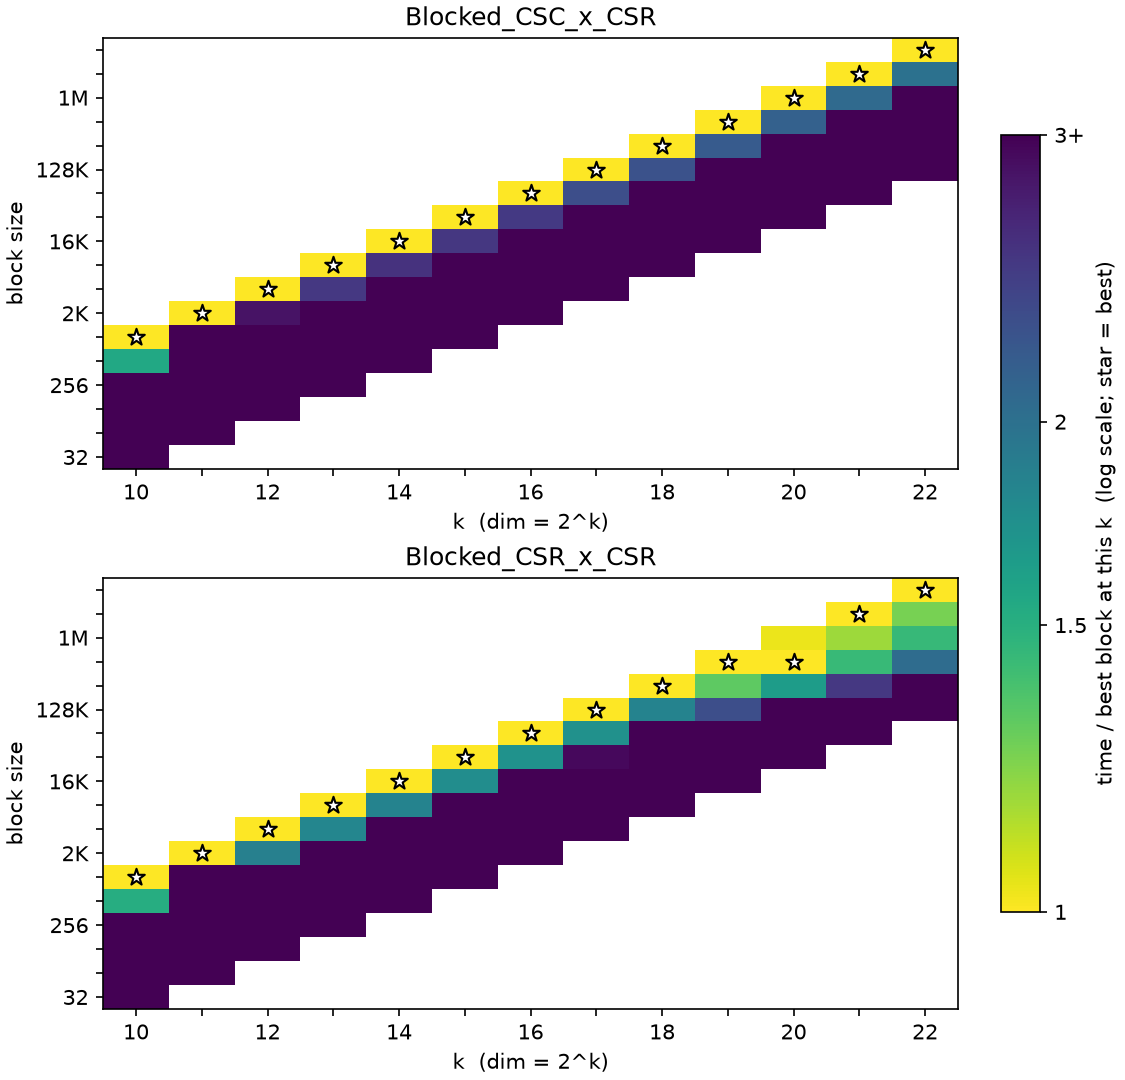
\includegraphics[width=0.9\linewidth,height=0.75\textheight,keepaspectratio]{figures/tiled_CA-Hep-Th_s2.png}
  \caption{CA-Hep-Th Sample 2 tiled block-size sweep. Colour is time relative to the best block size at each $k$ (1 is best); stars mark the best block size.}
  \label{fig:tiled_CA-Hep-Th}
\end{figure}
\clearpage

\begin{figure}[htbp]
  \centering
  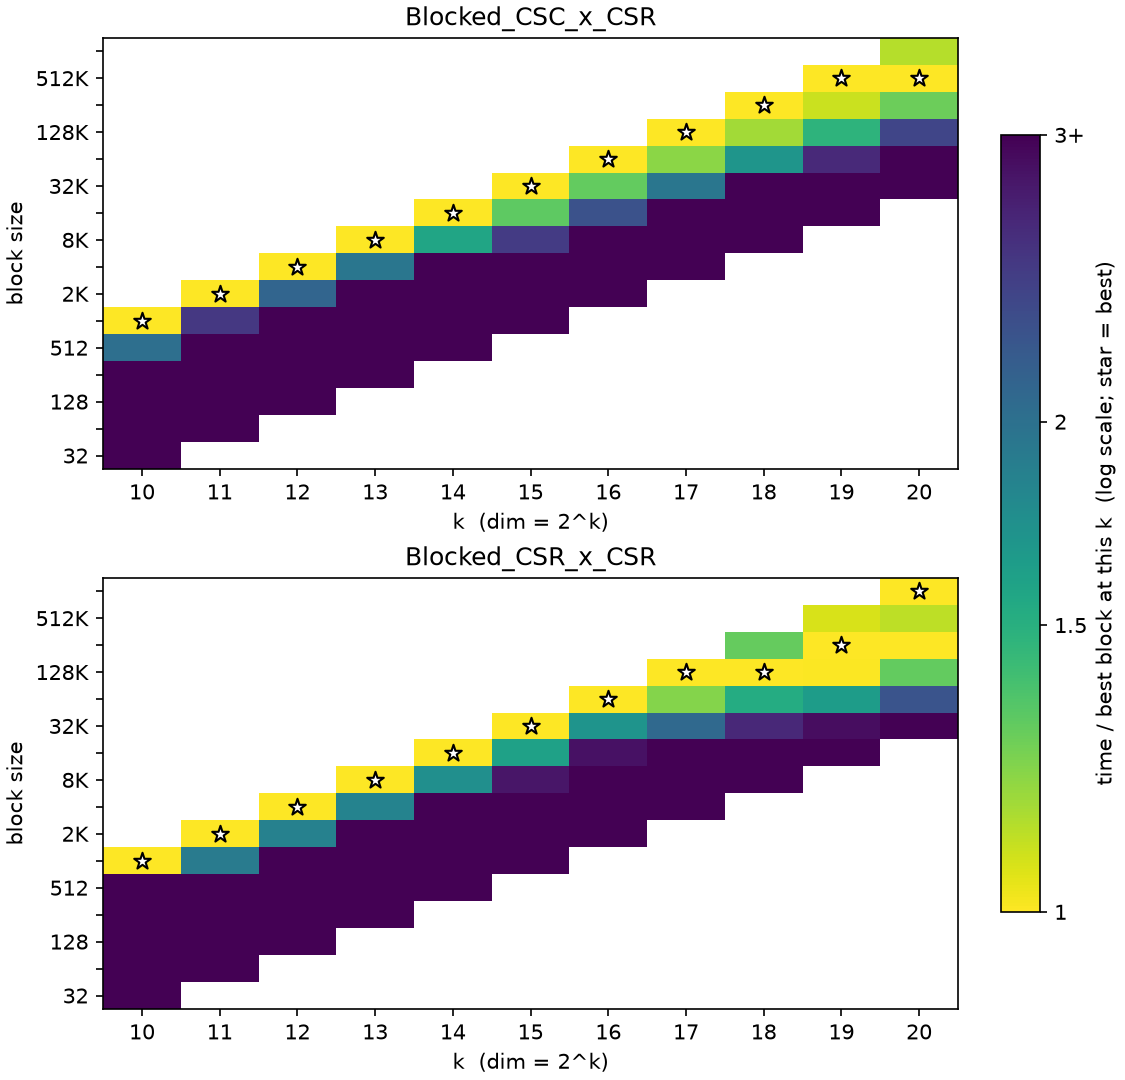
\includegraphics[width=0.9\linewidth,height=0.75\textheight,keepaspectratio]{figures/tiled_Cit-Hep-Ph_s2.png}
  \caption{Cit-Hep-Ph Sample 2 tiled block-size sweep. Colour is time relative to the best block size at each $k$ (1 is best); stars mark the best block size.}
  \label{fig:tiled_Cit-Hep-Ph}
\end{figure}
\clearpage

\begin{figure}[htbp]
  \centering
  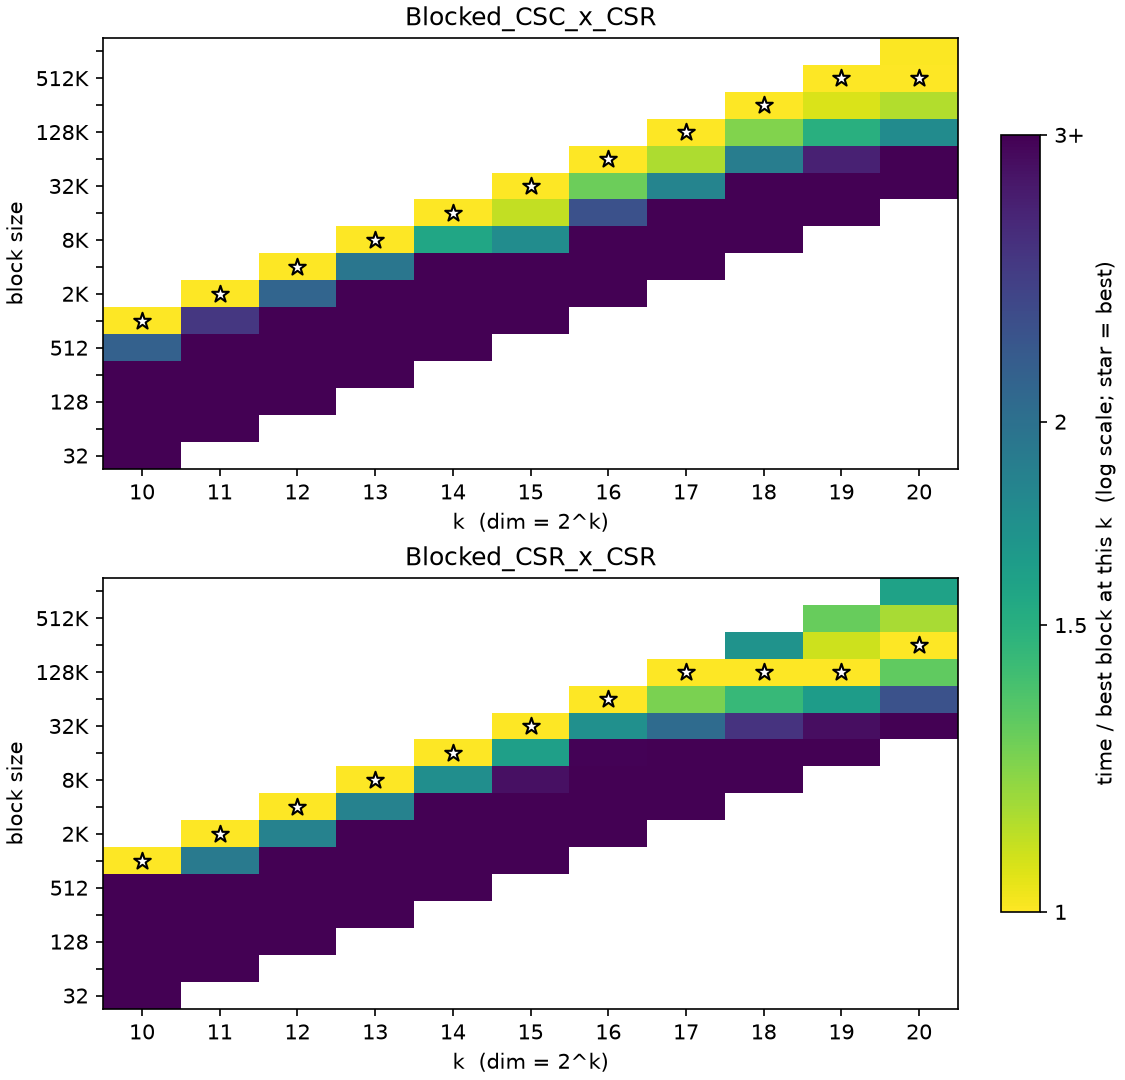
\includegraphics[width=0.9\linewidth,height=0.75\textheight,keepaspectratio]{figures/tiled_Cit-Hep-Th_s2.png}
  \caption{Cit-Hep-Th Sample 2 tiled block-size sweep. Colour is time relative to the best block size at each $k$ (1 is best); stars mark the best block size.}
  \label{fig:tiled_Cit-Hep-Th}
\end{figure}
\clearpage

\begin{figure}[htbp]
  \centering
  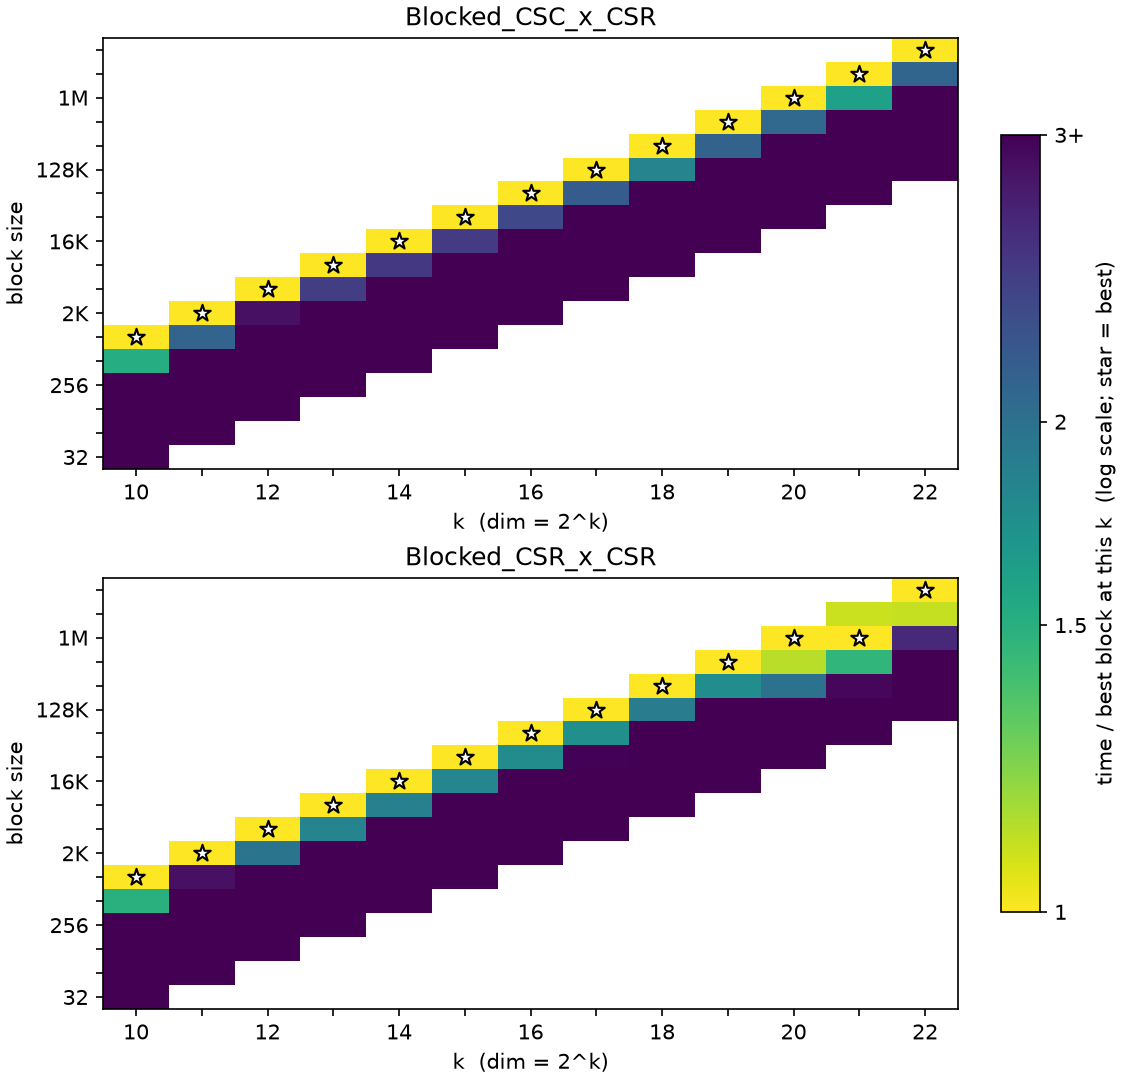
\includegraphics[width=0.9\linewidth,height=0.75\textheight,keepaspectratio]{figures/tiled_Delicious_s2.png}
  \caption{Delicious Sample 2 tiled block-size sweep. Colour is time relative to the best block size at each $k$ (1 is best); stars mark the best block size.}
  \label{fig:tiled_Delicious}
\end{figure}
\clearpage

\begin{figure}[htbp]
  \centering
  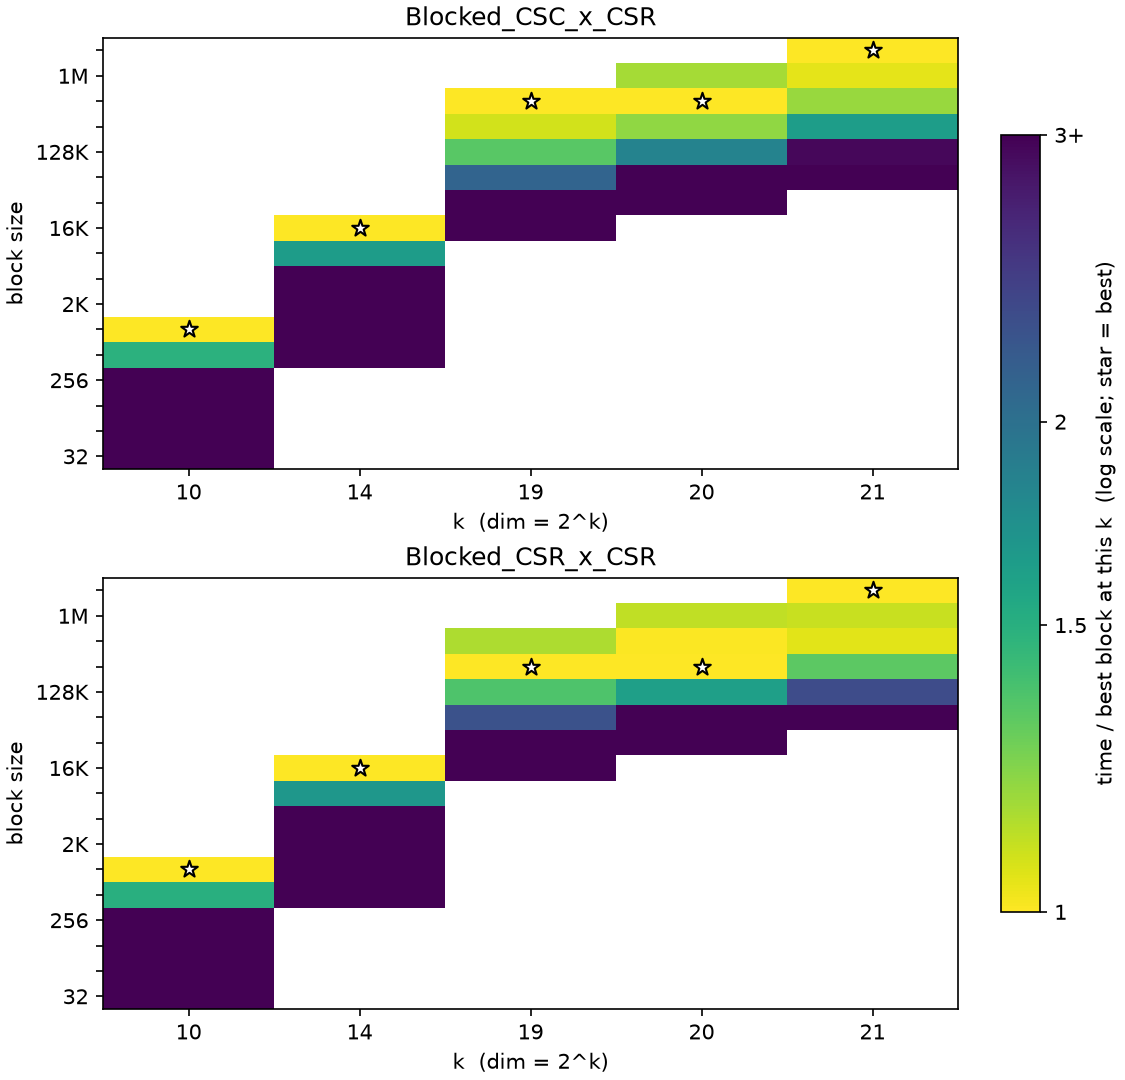
\includegraphics[width=0.9\linewidth,height=0.75\textheight,keepaspectratio]{figures/tiled_Epinions_s2.png}
  \caption{Epinions Sample 2 tiled block-size sweep. Colour is time relative to the best block size at each $k$ (1 is best); stars mark the best block size.}
  \label{fig:tiled_Epinions}
\end{figure}
\clearpage

\begin{figure}[htbp]
  \centering
  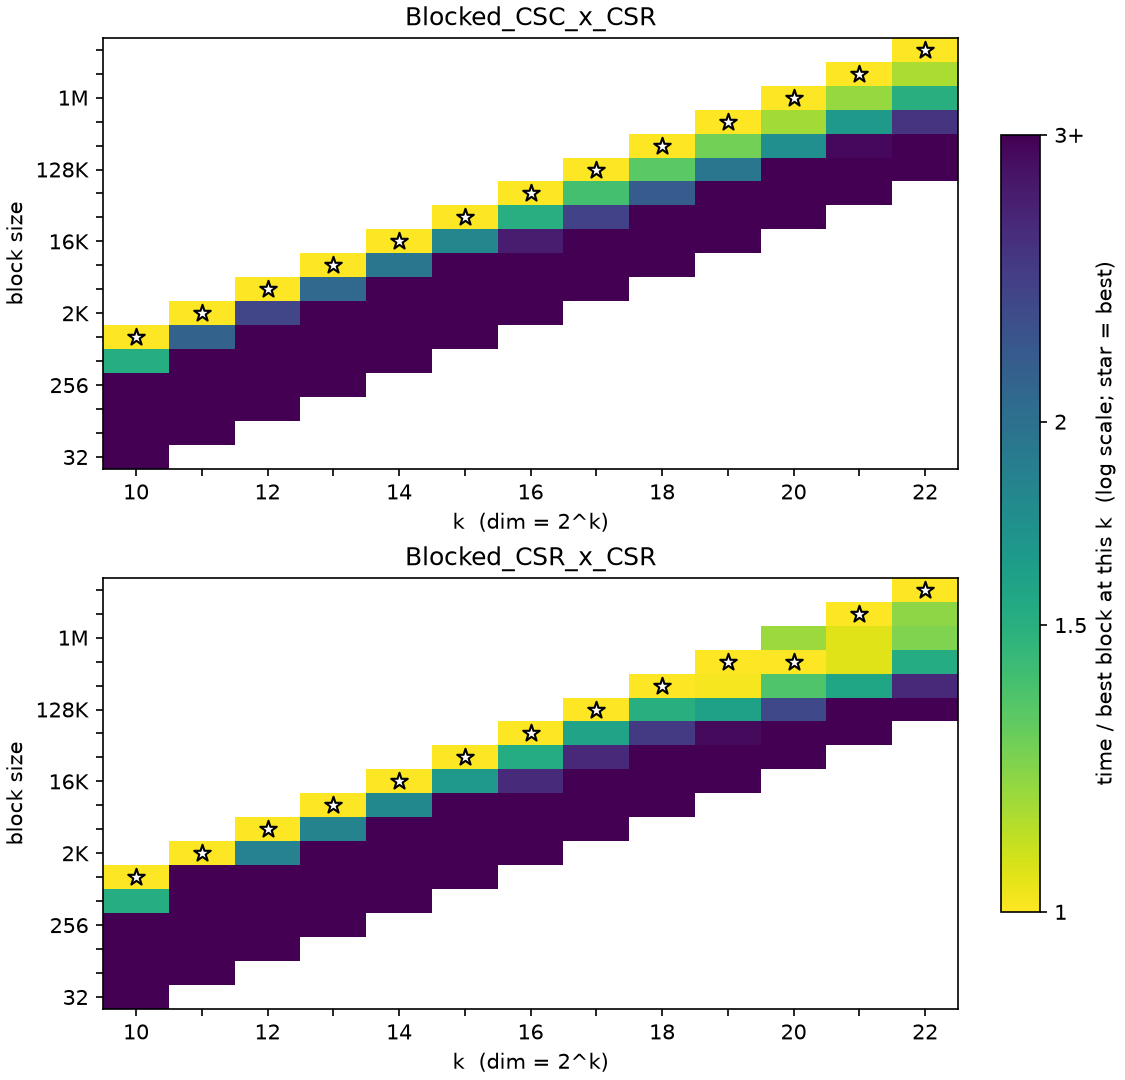
\includegraphics[width=0.9\linewidth,height=0.75\textheight,keepaspectratio]{figures/tiled_Flickr_s2.png}
  \caption{Flickr Sample 2 tiled block-size sweep. Colour is time relative to the best block size at each $k$ (1 is best); stars mark the best block size.}
  \label{fig:tiled_Flickr}
\end{figure}
\clearpage

\begin{figure}[htbp]
  \centering
  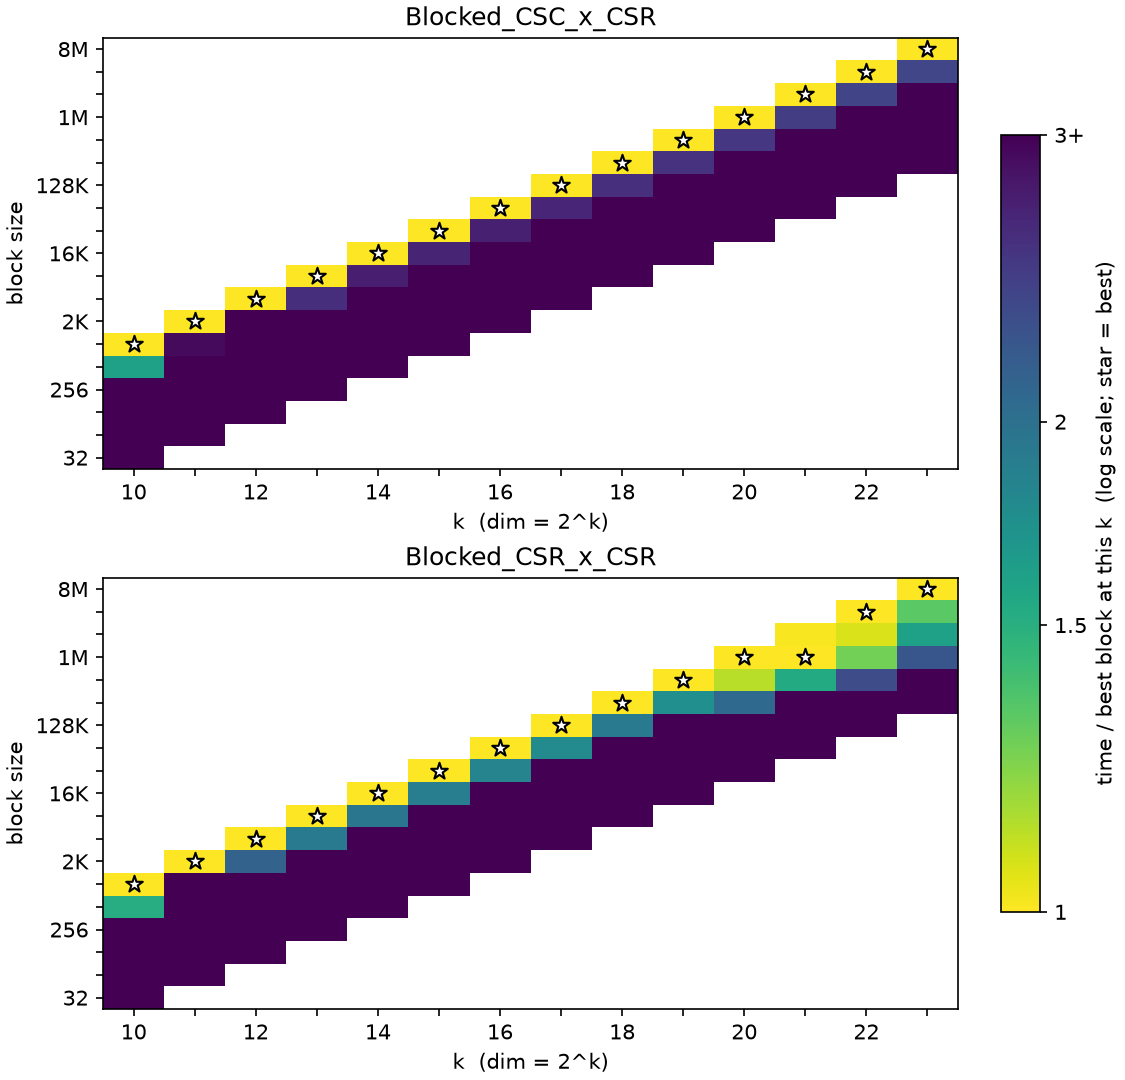
\includegraphics[width=0.9\linewidth,height=0.75\textheight,keepaspectratio]{figures/tiled_Gnutella-25_s2.png}
  \caption{Gnutella-25 Sample 2 tiled block-size sweep. Colour is time relative to the best block size at each $k$ (1 is best); stars mark the best block size.}
  \label{fig:tiled_Gnutella-25}
\end{figure}
\clearpage

\begin{figure}[htbp]
  \centering
  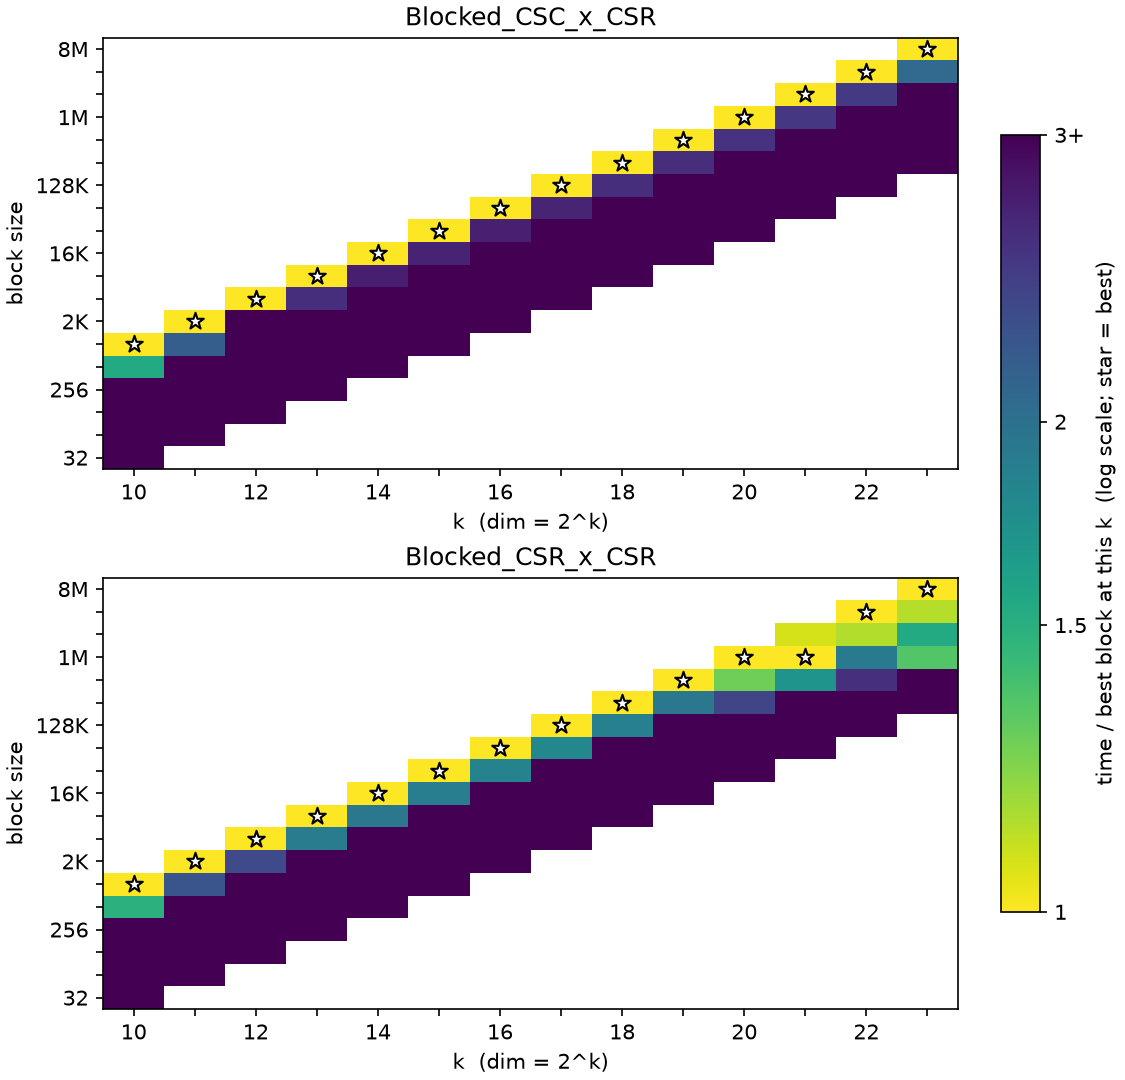
\includegraphics[width=0.9\linewidth,height=0.75\textheight,keepaspectratio]{figures/tiled_Gnutella-30_s2.png}
  \caption{Gnutella-30 Sample 2 tiled block-size sweep. Colour is time relative to the best block size at each $k$ (1 is best); stars mark the best block size.}
  \label{fig:tiled_Gnutella-30}
\end{figure}
\clearpage

\begin{figure}[htbp]
  \centering
  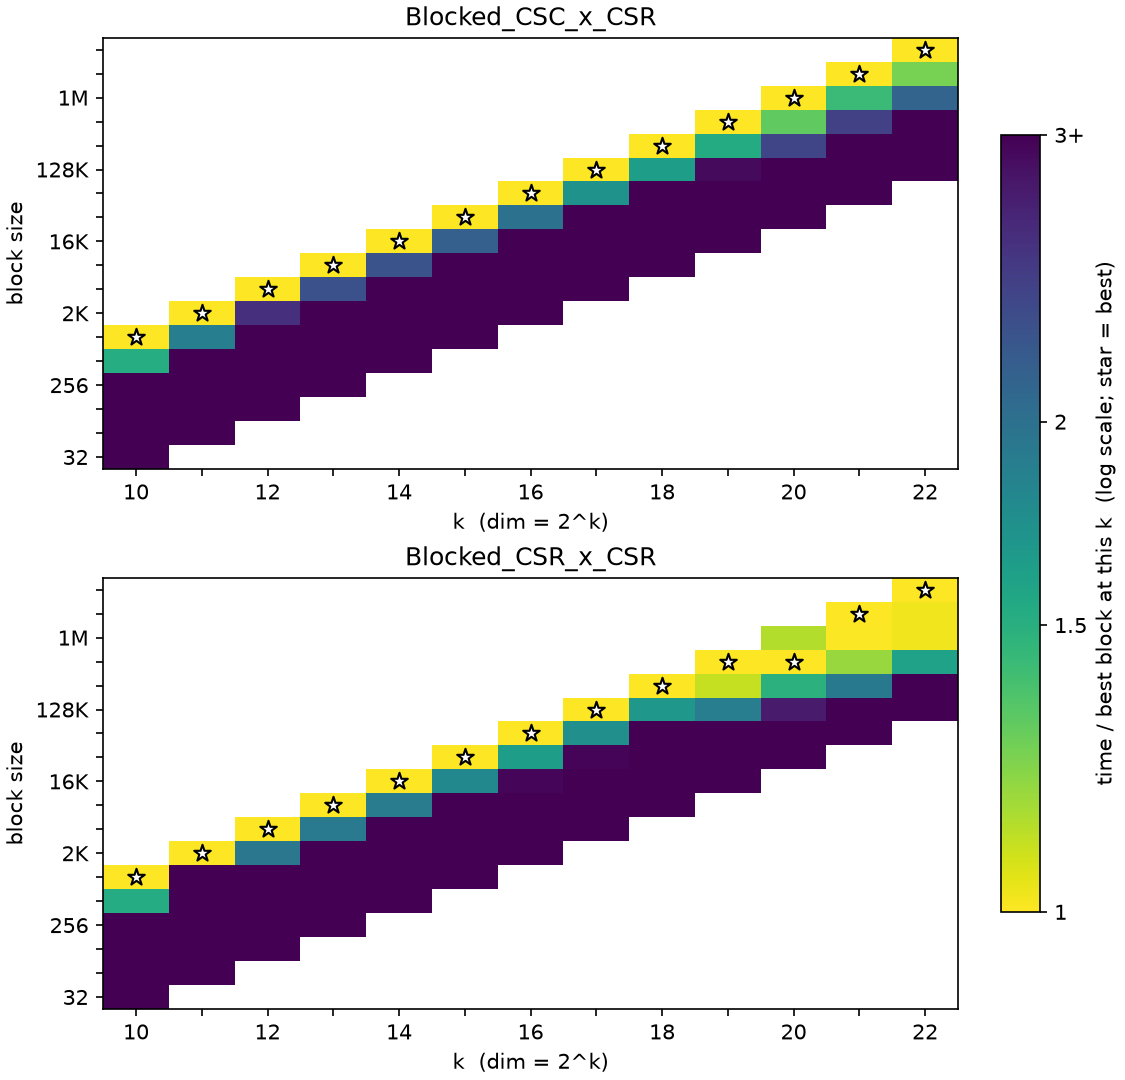
\includegraphics[width=0.9\linewidth,height=0.75\textheight,keepaspectratio]{figures/tiled_Web-Notredame_s2.png}
  \caption{Web-Notredame Sample 2 tiled block-size sweep. Colour is time relative to the best block size at each $k$ (1 is best); stars mark the best block size.}
  \label{fig:tiled_Web-Notredame}
\end{figure}
\clearpage
